\documentclass{article}

\usepackage{makeidx}
\usepackage{latexsym}
\usepackage{moreverb}
\usepackage{index}
\usepackage{subfigure}
\usepackage{boxedminipage}
\usepackage{fancybox}


\usepackage{ifpdf}
\newif\ifpdf
\ifx\pdfoutput\undefined
\else
  \ifx\pdfoutput\relax
  \else
    \ifcase\pdfoutput
    \else
      \pdftrue
    \fi
  \fi
\fi
\ifpdf
  \usepackage[pdftex,colorlinks=true,bookmarksopen, pdfstartview=FitH,
              linkcolor=blue, citecolor=blue, urlcolor=blue]{hyperref}
  \usepackage[pdftex]{graphicx}
  \pdfcompresslevel=9
\else
  \usepackage[dvips]{graphicx}
\fi


% ----------------------------------------------------------------
% HORIZONTAL MARGINS
% Left margin, odd pages: 1.25 inch (0.25 + 1)
\setlength{\oddsidemargin}{0.25in}
% Left margin, even pages: 1.25 inch (0 + 1)
\setlength{\evensidemargin}{0.25in}
% Text width 6 inch (so other margin is 1.25 inch).
\setlength{\textwidth}{6in}
% ----------------
% VERTICAL MARGINS
% Top margin 0.5 inch (-0.5 + 1)
\setlength{\topmargin}{-0.5in}
% Head height 0.25 inch (where page headers go)
\setlength{\headheight}{0.25in}
% Head separation 0.25 inch (between header and top line of text)
\setlength{\headsep}{0.25in}
% Text height 9 inch (so bottom margin 1 in)
\setlength{\textheight}{9in}
% ----------------
% PARAGRAPH INDENTATION
\setlength{\parindent}{0in}
% SPACE BETWEEN PARAGRAPHS
\setlength{\parskip}{\medskipamount}
% ----------------
% EMPTY BOXES OF VARIOUS WIDTHS, FOR INDENTATION
\newcommand{\hm}{\hspace*{1em}}
\newcommand{\hmm}{\hspace*{2em}}
\newcommand{\hmmm}{\hspace*{3em}}
\newcommand{\hmmmm}{\hspace*{4em}}
% ----------------
% VARIOUS CONVENIENT WIDTHS RELATIVE TO THE TEXT WIDTH, FOR BOXES.
\newlength{\hlessmm}
\setlength{\hlessmm}{\textwidth}
\addtolength{\hlessmm}{-2em}

\newlength{\hlessmmmm}
\setlength{\hlessmmmm}{\textwidth}
\addtolength{\hlessmmmm}{-4em}

\newcommand{\tbd}[1]{{\sf TBD: #1}}
\newcommand\lineup{\vspace*{-0.6em}}

\newcommand\com[1]{}
\newcommand{\te}[1]{\texttt{#1}}

% Library environment.  Used by generated code.
\newenvironment{libverbatim}
  {\small
   \verbatim}
  {\endverbatim
  }

\newsavebox{\fminibox}
\newlength{\fminilength}

\newenvironment{smbox}[1][2.5 in]
  {\begin{lrbox}{\fminibox}\begin{minipage}[c]{2.5 in}}
  {\end{minipage}\end{lrbox}\fbox{\usebox{\fminibox}}}


\newenvironment{fminipage}[1][6 in]
  {\begin{lrbox}{\fminibox}\begin{minipage}[c]{6 in}}
  {\end{minipage}\end{lrbox}\fbox{\usebox{\fminibox}}}

\newenvironment{smcenterboxverbatim}
  {\center
   \small
   \boxedverbatim}
  {\endboxedverbatim
  {\endcenter} }

\newenvironment{centerboxverbatim}
  {\center
   \boxedverbatim}
  {\endboxedverbatim
  {\endcenter }}


\newenvironment{codebox}
  {\VerbatimEnvironment
    \begin{center}
    \begin{Sbox}\begin{minipage}{5.7 in}\begin{Verbatim}}
  {\end{Verbatim}\end{minipage}\end{Sbox}
   \setlength{\fboxsep}{8pt}\fbox{\TheSbox}\end{center}}


\makeatletter
\def\subsubsubsection{\@startsection {subsubsubsection}{4}{\z@}{-3ex plus -1ex minus -.2ex}{1.25ex plus .2ex}{\normalsize\bf}*}
\makeatother

% ----------------------------------------------------------------
% ----------------------------------------------------------------
% HERE BEGINS THE DOCUMENT


% Create an index of Tcl commands, grouped by namespace
\makeindex
\newindex{commands}{cdx}{cnd}{Commands by Namespace}


\author{Revision: 19 October 2020}

\date{
Copyright {\copyright} 2020 Bluespec, Inc.   All rights reserved
}



\begin{document}


\title{
\resizebox{2in}{!}{
\includegraphics[width=\textwidth]{figures/B-Lang}}\\
\vspace{0.3in}
BSC Development Workstation \\
User Guide \\
\vspace*{1in}
\mbox{}
}

\maketitle

\newpage

\clearpage
\phantomsection
\addcontentsline{toc}{section}{Table of Contents}

\tableofcontents

\newpage


% ------------------------------------------------------------
% Section: Getting Started

\section{Getting Started}

% -------------------------

\subsection{Introduction}

\label{sec-intro}

This document explains the mechanics and logistics of compiling,
simulating, and analyzing a Bluespec SystemVerilog (BSV)
specification with the BSC Development Workstation (BDW).
BDW is a full-featured graphical 
environment  designed for BSV. You can create, edit,
compile,  simulate, analyze, and
debug  BSV designs from within the Workstation or from the
command line.   You can choose the
editors, simulators, and waveform viewers to  use along with
Bluespec-based analysis tools. The Development
Workstation builds on  Bluetcl, a collection of Tcl extensions,
scripts, and packages providing Bluespec-specific features to Tcl.

For a reference of Bluetcl commands, please refer to the BSC
documentation.

For information on how to design and write specifications in the
Bluespec SystemVerilog environment, please refer to the
{\em Bluespec SystemVerilog Reference Guide}, {\em BSV by Example} guide,
and other tutorials provided by Bluespec Inc or the B-Lang organization.

% -------------------------

\subsection{Installing BSC and BDW}
\index{installing}
\label{sec-installation}

% -----

\subsubsection{Download the software}

TBD

% -----

\subsubsection{System Requirements}

TBD

To view graphs within the Development Workstation,
Tcldot 2.21 or later must be installed.  Requirements for viewing graphs
are discussed in Appendix \ref{graphviz-install}. 

% -----

\subsubsection{Install the software}

TBD

% -------------------------

\subsection{Quick Start}

Once BDW is installed,
% and any optional Unix environment variables are set,
execute the command \te{bdw} to start the Development Workstation:

\begin{centerboxverbatim}
bdw
\end{centerboxverbatim}

This command brings up main Workstation window, from which you can perform
all BSC tasks.

You can also add the name of an existing BDW project file as you start
the Workstation:

\begin{center}
\begin{smbox}
{\tt \hspace*{2em} bdw}\hspace*{2em}\emph{project}{\tt .bspec}
\end{smbox}
\end{center}

where \te{project.bspec} is the project file name.  This
starts the Workstation and opens the project.  The project file contains
the saved project preferences and settings.

% ------------------------------------------------------------
% Section: Designing with Bluespec

\section{Designing with Bluespec}

% -------------------------

\subsection{Components of a BSV Design}

A BSV program consists of one or more outermost constructs called
packages.  All BSV code is assumed to be inside a package.  Furthermore, the
BSV compiler and other tools assume that there is one package per
file, and they use the package name to derive the file name.  For
example, a package called \texttt{Foo} is assumed to be located in the file
\texttt{Foo.bsv}.


When using the BSC Development Workstation you will also have a
project file, ({\em projectname}\te{.bspec}), which is a saved
collection of options and parameters.  Only the Development
Workstation defines project files;  you
do not have a \te{.bspec}
project file if you use BSC completely from the Unix command line.

The design may also include Verilog modules, VHDL modules,  and C functions.
Additional files will be generated as a result of the  compile, link,
and simulation tasks.
 Some files are only generated for a
particular back end (Bluesim or Verilog), others are used by both
back ends.  The following table lists the different
file types and their roles.

\begin{center}
\index{file types}
\index{.bsv@\te{.bsv} (file type)}
\index{.bo@\te{.bo} (file type)}
\index{.ba@\te{.ba} (file type)}
\index{.v@\te{.v} (file type)}
\index{.h@\te{.h} (file type)}
\index{.o@\te{.o} (file type)}
\index{.cxx@\te{.cxx} (file type)}

\begin{tabular}{|p{.5 in}|p{2.5 in}|p{.5 in}|p{.5 in}|}
\hline
\multicolumn{4}{|c|}{ } \\
\multicolumn{4}{|c|}{File Types in  a BSV Design}\\
\hline
&&&\\
\multicolumn{1}{|c|}{File
Type}&\multicolumn{1}{|c|}{Description}&\multicolumn{1}{|c|}{Bluesim}&\multicolumn{1}{|c|}{Verilog}\\&&&\\
\hline
\te{.bsv}&BSV source File&$\surd$&$\surd$\\
\hline
\te{.bspec}&Workstation project File&$\surd$&$\surd$\\
\hline
\multicolumn{4}{|l|}{The \te{.bo} file is an intermediate
file not viewed by the user}\\
\hline
% \te{.bi}&Text file containing information about the items exported from the
% package&$\surd$&$\surd$\\
% \hline
\te{.bo}&Binary file containing code for the package in an
intermediate form&$\surd$&$\surd$\\
\hline
\multicolumn{4}{|l|}{}\\
\hline
\te{.ba}&Elaborated module file&$\surd$&$\surd$\\
\hline
\te{.v}&Generated Verilog file &&$\surd$\\
\hline
\multicolumn{4}{|l|}{}\\
\hline
\te{.h}&\te{C++} header files &$\surd$ &\\
\hline
\te{.cxx}&Generated \te{C++} source file&$\surd$ &\\
\hline
\te{.o}&Compiled object files &$\surd$ &\\
\hline
\te{.so}&Compiled shared object files &$\surd$ &\\
\hline
\end{tabular}
\end{center}

% -------------------------

\subsection{Overview of the BSC process}

Designing with BSC has three distinct stages.  You can use the
BSC Development Workstation throughout each stage of the process.
Figure \ref{compiler-stages-fig} illustrates the following
steps in building  a BSV design:
\begin{enumerate}
\item A designer writes a BSV program, including Verilog, VHDL,  and C components as desired.
\item The BSV program is  compiled into a Verilog or Bluesim
specification. This step is comprised of two distinct stages:
\begin{enumerate}
\item pre-elaboration - parsing and type checking
\item post-elaboration - code generation
\end{enumerate}
\item  The compilation output is either linked  into a simulation
environment or processed by a synthesis tool.
\end{enumerate}

\begin{figure}[ht]
  \centerline{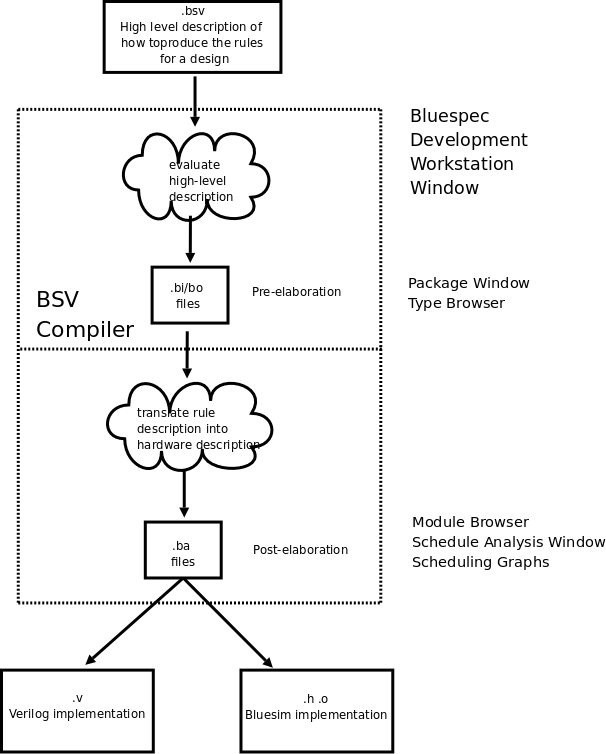
\includegraphics[angle=0, height=4.5in]{figures/compilerstages}}
  \caption{\label{compiler-stages-fig}BSC compilation stages}
\end{figure}


We  use the {\em compilation}\index{compile} stage to refer
to the two steps, type checking  and code generation, as shown inside
the dotted box in Figure \ref{compiler-stages-fig}. As the figure
shows, the  code generation specification that is output
by BSC is subject to a second run of the compiler to link
it into a simulation or synthesis environment.  We  refer to this
as the \index{link}
{\em linking} stage, even though the same compiler is used to perform
the linking.
BSC is required for
linking Bluesim generated modules.  For Verilog, the generated modules
can be handled as you would any other Verilog modules; they can be
linked with BSC or you can choose to use the
generated Verilog files manually instead.

You perform the above actions: compile, link, and simulate, from the
{\bf Build} menu (Section~\ref{build}) in the Development Workstation.

Once you've generated the Verilog or Bluesim implementation, the
 Development Workstation provides the following  tools to help
 analyze your design:
\begin{itemize}
\item Interface with an external waveform viewer, with additional BDW-provided
 annotations, including  structure and type definitions
\item Schedule Analysis viewer providing multiple perspectives of a
module's schedule
\item Scheduling graphs providing a graphical display of schedules,
conflicts, and dependencies among rules and methods.
\end{itemize}

% -------------------------

\subsection{Overview of the BSC Workstation}

% -----

\subsubsection{Workstation Windows}

The Workstation consists of a set of windows and browsers  providing
different views of the design.  The particular window used for a task
depends on the information you want to see and the stage of the
design.    The following table summarizes the
windows and browsers in the Workstation.


\begin{center}
\begin{tabular}{|p {1 in}|p {1.6 in}|p {2.8 in}|}
\hline
\multicolumn{3}{|c|}{BSC Workstation Windows}\\
\hline
Stage&Window&Function \\
&&\\
\hline
\hline
All &
Main Window&Central control window.   Manage projects, set project
options, build projects, and  monitor status. \\
\cline{2-3}
&Project Files Window&View, edit and compile  files in the
project.  \\
\hline
Pre-elaboration&
Package Window&  Load
packages into the Workstation and browse their contents.  Provides a
high-level view of the types, interfaces, functions and modules
defined in the package.\\
\cline{2-3}
&Type Browser&Primary means for viewing information about types and
interfaces.  Displays the full structure hierarchy and all the
concrete types derived from resolution of polymorphic types.\\
\hline
Post-elaboration&
Module Browser& Displays the design hierarchy and an overview
of the contents of each module.   Links to  external
 waveform viewers.\\
\cline{2-3}
&Schedule Analysis Window&View  schedule
information including warnings, method calls, and conflicts between rules for a module. \\
\cline{2-3}
&Scheduling Graphs& Graphical view of schedules, conflicts, and dependencies.\\
\hline
\end{tabular}
\end{center}




Within the Development Workstation  you  choose the editors,
Verilog simulators, and waveform viewers  to use along with
Bluespec-specific analysis tools.
The following third-party products can be accessed from the
Workstation but are not provided with BDW or BSC:
\begin{itemize}
\item Editors:  gvim and emacs
\item Verilog Simulators: modelsim, ncverilog, vcs/vcsi, cver/cvc,
iverilog,  veriwell, and isim\footnote{isim  version 11.3 or later}
\item Waveform Viewers: SpringSoft/Novas (Verdi, Debussy, nWave), GtkWave
\item Graph Software: graphviz
\index{graphviz}(Section \ref{graphviz-install}) which includes Tcldot \index{Tcldot}
\end{itemize}


% The package graphviz, including the Tcl extensions, must be installed
% to use the scheduling graphs in the Development Workstation. The graphviz
% Tcl extensions (Tcldot) must be compatible with Tcl 8.5 (Tcldot
% version 2.21 or greater) to work with the
% Development Workstation.  You may need to adjust the autopath for the
% graphvix package in the file \te{\$HOME/.bluetclrc} for your
% installation.    For more information on installing and using Tcl,
% refer to the many resources available on the web, including \te{www.tcl.tk/doc}.

% -----

\subsubsection{Using the Main Window}

The {\bf Main} window, as shown in Figure \ref{fig-main},
is the control center of the BSC Development Workstation.
From this window you can manage projects, set project
options, and monitor status while working in the Development
Workstation. The window displays all commands executed in addition to
warnings, errors, and messages generated by BSC
and the Development Workstation.

\begin{figure}[ht]
\begin{center}
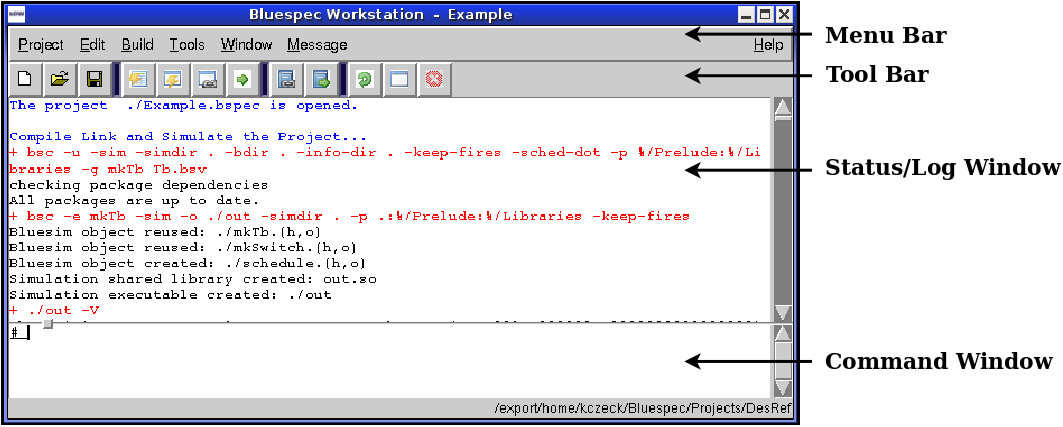
\includegraphics[width = 6 in]{figures/mainwindow}
\caption{Main window components}
\label{fig-main}
\end{center}
\end{figure}

The main window consists of the following components:
\begin{itemize}
\item The {\bf menu bar}, from which you can launch  all actions.
\item The {\bf toolbar},  a set of icons implementing shortcuts for
frequently used actions.  All toolbar icons  also appear as menu bar items.
\item The {\bf status/log window} displaying commands, project status,
messages, warnings, and errors.
\item The {\bf command window} where you can enter \index{Tcl} Tcl
commands.  All
actions available through the Development Workstation user interface have analogous
Tcl commands. (Refer to Appendix \ref{tcl-commands} for the full description of supported
commands).
\end{itemize}

% -----

\subsubsubsection{Menus}

All actions in the Workstation can be accessed from the menu bar in
the main window.  The menus are:

\begin{itemize}
\item {Project:} Actions applied to the entire project, such as
opening, closing, creating a new project, and project settings,
including window placement settings.
\item {Edit:} Clipboard (copy/paste) actions and Workstation font settings.
\item {Build:} Actions applied to the design, such as compiling and
simulating.
\item {Tools:} Built-in Workstation tools, to facilitate working with
Bluespec designs.
\item {Window:} Actions to manage (open/close/minimize) the Workstation windows.
\item{Message:} Actions applied to the messages in the message window.
\item{Help:} Access all product documentation, including labs and
tutorials.  Display the version of the Workstation you are running.
\end{itemize}

% -----

\subsubsubsection{Messages}
\index{compiler messages}
The messages displayed in the status/log window are generated by both BSC and the Development
Workstation and  are color-coded by type as follows:
\begin{itemize}
\item{red:}  error or warning from the compiler

\item{black:} a result or status from the compiler (example - compiling)
\item{dark red:} error from the Development Workstation

\item{blue:} information from the Development Workstation (example - compile finished)
\end{itemize}

The red and black messages are the same messages returned by BSC on the
command line while the dark red and blue messages are generated by the
Development Workstation. When the compiler returns errors or warnings (red
messages), you can double-click on the message to open the file at the
specified line.

The format of the messages displayed in the status/log window can be
modified from the {\bf Message} menu.
The {\bf Hide Messages}  option decreases the  font of
informational messages  to
emphasize  warning and error messages.   {\bf Show Messages} sets
all message fonts to the same size.

% -----

\subsubsubsection{Command Line}
The Workstation command line is a prompt to a Tcl shell.  All standard Tcl as well
 as  Bluetcl commands can be executed from this prompt.  You can
also write your own Tcl commands, procs, and scripts using any
combination of Tcl and Bluetcl commands.  These must be added to the
 \te{.bluetclrc} file before you
 can execute them from the Development Workstation command line.
 Section~\ref{custom} for more information on customizing with Bluetcl and  the
 Development Workstation.

To display the list of available Bluetcl commands, type
\te{Bluetcl::help} at the Workstation command line.  To display the
list of Workstation Bluetcl commands, type \te{WS::help -list}.  For
more information on Bluetcl commands refer to  the Bluetcl reference
guide.

% -----

\subsubsection{Keyboard shortcuts in the Workstation}

All of the menu options have keyboard shortcuts which allow you to
perform an action from the  keyboard instead of using the mouse.
To open a project, for example, you  type \te{Alt-P} (for the
Project menu), followed by \te{Alt-O} (for open), as shown in Figure \ref{fig-hotkey}.  This will bring up
the {\bf Open Project} menu.  The keyboard shortcut is indicated by
the underlined letter in each menu item.

\begin{figure}[ht]
\begin{center}
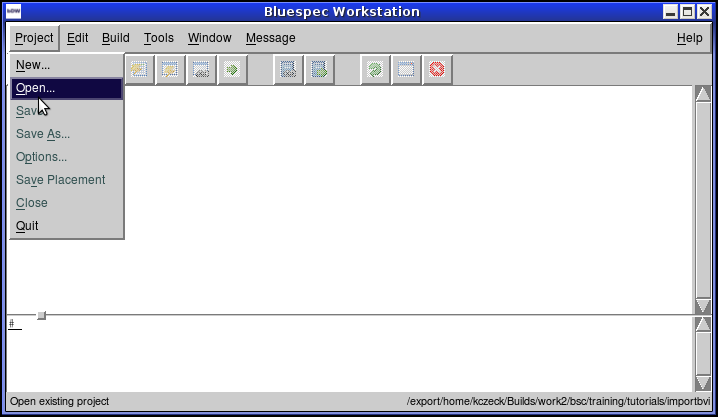
\includegraphics[width = 4 in]{figures/open}
\caption{Project Menu Hotkeys}
\label{fig-hotkey}
\end{center}
\end{figure}


Most standard hotkeys are available in the Workstation including the
following:
\begin{itemize}
\item Cntl w: close active window
\item up arrow, down arrow: move up or down on a list
\item $\rightarrow$: expand hierarchy
\item $\leftarrow$: collapse hierarchy
\item Cntl + or Cntl = : increase the Workstation \index{font size}font by 1 point
\item Cntl - : decrease the Workstation font by 1 point
\end{itemize}

% ------------------------------------------------------------
% Section: Managing Projects

\section{Managing Projects}

The basic unit of work within the BSC Development Workstation is the
{\bf Project}.   The project file ({\em projectname}\te{.bspec})  is
a named collection  of project settings and options.  You manage
(open, create, save, close)
projects from the {\bf Project} menu.  You  modify the project options
through the {\bf Project$\rightarrow$Options} menu, described in
Section~\ref{project-options}.

% \begin{figure}[ht]
% \begin{center}
% 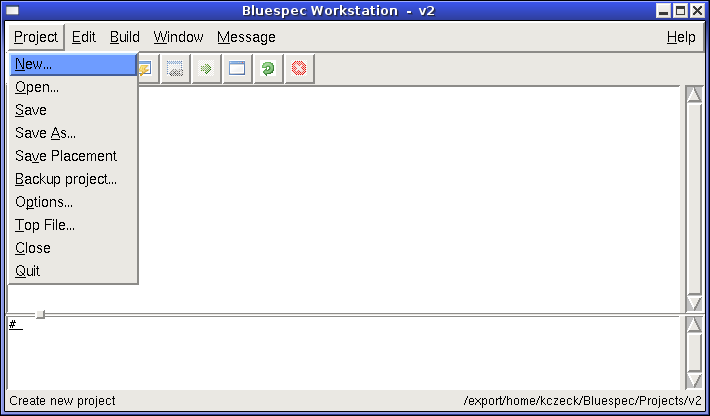
\includegraphics[width = 4 in]{figures/projectmenu}
% \caption{Project Menu}
% \label{fig-projectmenu}
% \end{center}
% \end{figure}

% -------------------------

\subsection{Creating a Project}

\label{project}
\index{project}
\index{.bspec@\te{.bspec}}



When you create a new project in the BSC Development Workstation,
 a {\em projectname}\te{.bspec} file is created.

% A single set of Bluespec files can be
% used in  multiple projects.  In
% this case multiple \te{.bspec} project files could point to the same
% directory or directories containing the Bluespec design files.

\begin{figure}[ht]
\begin{center}
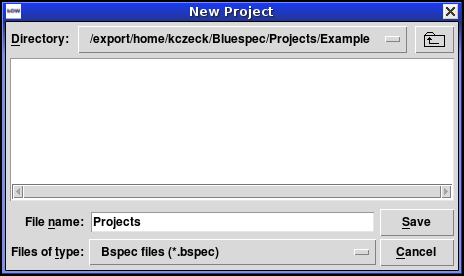
\includegraphics[width = 3 in]{figures/newproject}
\caption{New Project Window}
\label{fig-new}
\end{center}
\end{figure}

To create a new project,  select {\bf New} from the {\bf Project} pull-down
menu.  Select a directory and enter a file name on  the {\bf New Project} dialog window, shown in Figure \ref{fig-new}.
The directory must already exist, but it may be empty or
 populated with
\te{.bsv} files.  There may even already be an existing \te{.bspec}
file.  {\em New} indicates that you want to define a new project,
creating  a new \te{.bspec} file, even if it uses files in a directory already
included in another project.

% The Project Directory and
% BSC library files are automatically added to the
% search path of the project.    Once the project is created, add any additional
% directories to the search path via the {\bf Project
% Options$\rightarrow$Files} tab, as described in Section
% \ref{options-searchpath}.

After you press {\bf Save} to close the {\bf New Project} window, the
{\bf Project Options} window will open, so you can set up your project.

\index{default project settings}
\index{settings!default}
Your project defaults may differ from the defaults programmed into
the Workstation.  To create your own project default settings, create a 
project and set the project options to  your preferred defaults.   Then, when
creating a new project, {\bf Open} the {\em default} project instead
of creating a new project, and {\bf Save as} under your project name.

% The top file and top module fields can be
% entered as the project is created, or left blank until you are ready
% to compile.
%  The top file contains the top synthesized module of the
% hierarchy which
%  imports all other files and modules used in the design.
% To compile a design, the top file must be specified.  To link,
% the  top module must also be specified.  These may be defined when the
% project is created or  specified in {\bf Files} tab of the
% the {\bf Project Options} window.

% If you have successfully compiled your project, and the {\bf Link}
% option is still not available, confirm that the  top module has
% been specified.

% -------------------------

\subsection{Setting Project Options}
\label{project-options}
\index{options}
\index{settings!Project Options menu}

Once a project is created, the user options are modified through the {\bf Project$\rightarrow$Options} menu.
The {\bf Options} window contains the following  tabs:
\begin{itemize}
\item Files
\item Compile
\item Link Simulate
\item Editor
\item Waveform Viewer
\end{itemize}

All of the fields in the {\bf Options} tabs
correspond either to bsc compiler flags or values passed to the bsc
compiler, as described in the BSC documentation.
For a full listing of all bsc compiler flags, type:
\begin{centerboxverbatim}
exec bsc -help
\end{centerboxverbatim}
in the Workstation command window or:
\begin{centerboxverbatim}
bsc -help
\end{centerboxverbatim}
from a Unix command prompt.

% -----

\subsubsection{Meta Variables}
\label{metavariable}

\index{meta variables}
\index{meta variables!\%P}
\index{meta variables!\%M}
\index{meta variables!\%B}

\index{\%P (meta variable)}
\index{\%M (meta variable)}
\index{\%B (meta variable)}

The Development Workstation stores some commonly used values in meta
variables.  These variables can be used in the option fields, in
Makefiles, and in custom
command fields for compiling, linking and simulating from the Workstation.


\begin{center}
\begin{tabular}{|l|l|l|}
\hline
\multicolumn{3}{|c|}{}\\
\multicolumn{3}{|c|}{\bf Meta Variables Defined in the Workstation}\\
\hline
{\bf Variable}&{\bf Value}&{\bf Description}\\
\hline
\hline
\%P&Top File&Top file of the project\\
\hline
\%M&Top Module&Top module of the project\\
\hline
\%B&\$BLUESPECDIR&\te{install\_directory/lib}\\
\hline
\end{tabular}
\end{center}

% -----

\subsubsection{Files}
\label{options-files}

The {\bf Files} tab, shown in Figure \ref{fig-files},  contains the following options:
\begin{itemize}
\item Top File and Top Module
\item Location of generated and included files
\item Search path directories
\item Display criteria
\item Copy flags option
\end{itemize}

The following table
shows the fields on the {\bf Files} tab along with the associated
compiler flags.
When you compile from the Workstation, the Workstation supplies the
appropriate compile flag and value to the \te{bsc} command.

\begin{figure}
\begin{center}
\begin{tabular}{|p{1 in}|p{.75 in}|p {.75 in}|p {3 in}|}
\hline
&&&\\
{\bf Field} &{\bf flag}&{\bf Task}&{\bf Description}\\
\hline
\hline
Top Module& -e&Link&Specifies the top-level module for simulation\\
\hline
.bo/.ba files & -bdir&Compile & output directory for .bo/.ba files\\
\hline
Bluesim files & -simdir&Compile& output directory for Bluesim intermediate files\\
\hline
Verilog files& -vdir&Compile & output directory for .v files\\
\hline
Info Files& -info-dir&Compile& output directory for informational files\\
\hline
Search Path& -p&Compile&directory path for source and intermediate files\\
\hline
\end{tabular}
\end{center}
\caption{Compiler flags by Field}
\label{fieldtable}
\end{figure}


\begin{figure}[ht]
\begin{center}
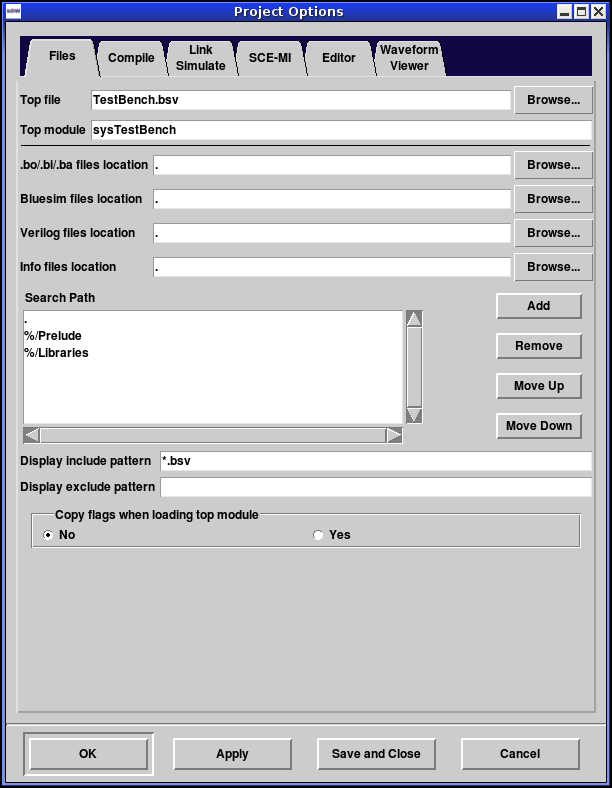
\includegraphics[width = 3 in]{figures/options-files}
\caption{Compiler Options - Files}
\label{fig-files}
\end{center}
\end{figure}


\paragraph{Top File and Top Module}

 The top file contains the top package, which includes the  top
synthesized module of the hierarchy.  The top file imports all other files
 all other files and modules used in the design.
To compile a design, the top file must be specified.  To link,
the  top module must also be specified.   The value of the top file
and top module
fields are stored in the \te{\%P}\index{\%P (meta variable)} (file)
and \te{\%M} \index{\%M (meta variable)} (module) meta variables.



\paragraph{Files Location}

The 4 files location fields  indicate where output files should be placed
during build tasks, as well as where the Development
Workstation looks for the generated files.
 The  default is in
the directory in which the input files reside.   The table in Figure
\ref{fieldtable} lists the   location
fields and their  corresponding compiler flags.

\index{search path}
\index{settings!search path}
\label{options-searchpath}

\paragraph{Search Path}
The Search Path contains the default locations where the compiler
looks for source and intermediate files.  These are the directories
supplied to the \te{-p} flag.

When a project is created in the Development Workstation, the
following directories are automatically added to the search path:
\begin{itemize}
\item{\bf .}: the project directory
\item {\bf \%/Libraries}: additional compiled BSC library packages
\end{itemize}

 \% is the \te{\{\$BLUESPECDIR\}} environment
variable, which gives the \te{lib} directory in the BSC installation.  This
value is stored in the Workstation meta variable \te{\%B}\index{\%B (meta variable)}.

You can add, remove, and reorder directories in the search path.


\paragraph{Display patterns}
The display include and exclude patterns are used by the {\bf Project
Files} window to determine which files from  the project path to display.
The files displayed  are selected by
file extension.   By default,
all files  in the search path with an
extension of \te{.bsv} are displayed in the {\bf Project Files}
window.  In this tab  you can add patterns to include or exclude.  For
example, you may want to display Verilog files in the search path, in
which case you would add \te{*.v} to the include patterns.   Or if you
wanted to display all files, except for \te{.bo} files,
you would specify \te{*.*} for the {\bf Include Patterns} and
 \te{*.bo} for the {\bf Exclude Patterns}.


\paragraph{Copy flags when loading top module}
Loading the top module means loading the \te{.ba} file for the
compiled design.  If the design was built (compiled) outside of the
Workstation, or in another session of the Workstation, the compile
flags used for the compilation may not match the compile flags set in
the {\bf Options} window.  By selecting {\bf Yes}, the flags are
copied from the \te{.ba} file into the {\bf Project Options}.  
If you don't copy the options, you may not see the correct signal names 
 in the waveform viewer.

% -----

\subsubsection{Compile}
\index{compile options}
\index{settings!compile options}
\label{compiler-options}

\begin{figure}[ht]
\begin{center}
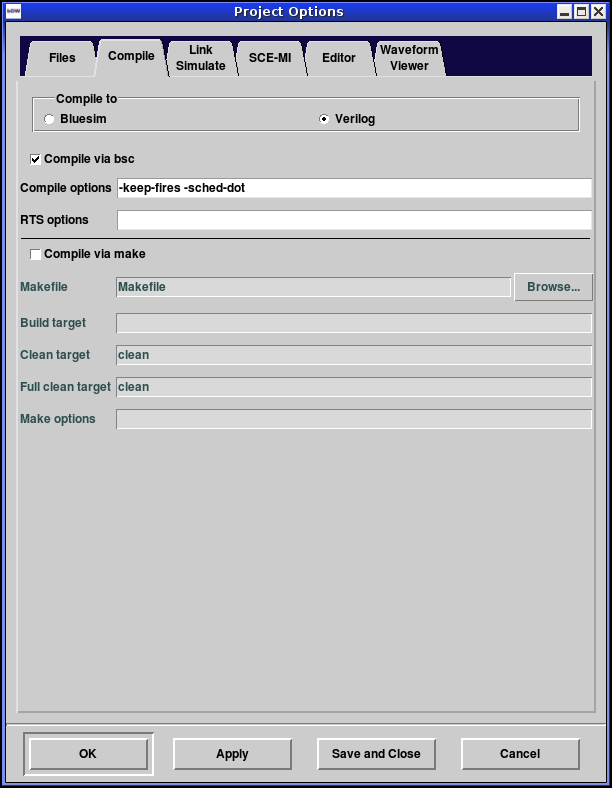
\includegraphics[width = 3 in]{figures/options-compile}
\caption{Project Options - Compile}
\label{fig-compiler1}
\end{center}
\end{figure}

The {\bf Compile} tab, shown in Figure \ref{fig-compiler1},  is where you indicate whether you are compiling
to Bluesim or Verilog.  This is the same value as on the  {\bf Link/Simulate}
tab.

The rest of the tab is divided into two sections; one section
contains options for when you are compiling via bsc, the other for when
you are using a makefile.

There are two additional fields when the compilation type is {\bf\tt
bsc}, compile options and RTS options.  Compile options are any of the
BSC compile flags, while the RTS options are the run-time system's
 \te{-Hsize} and \te{-Ksize} flags, as described in the BSC documentation.
All bsc compiler flags
should be typed in exactly as they would be on the command line.  When
you compile the project, the specified flags will be applied.
The following
table lists the field on the {\bf Compile} tab and the associated bsc
compiler flags.

\begin{center}
\begin{tabular}{|p{1 in}|p{1 in}|p {3 in}|}
\hline
{\bf Field} &{\bf Compiler flag}&{\bf Description}\\
\hline
\hline
Bluesim & -sim & Compiles for Bluesim\\
\hline
Verilog & -verilog&Compiles for Verilog\\
\hline
Compile options & bsc flags & See BSC documentation\\
\hline
RTS options&-Hsize&Maximum heap size\\
&-Ksize&Maximum stack size\\
\hline
\end{tabular}
\end{center}


\index{compiler flags, using}

\index{makefile!using}
When the compilation type is {\bf\tt make},  you can specify the
following fields.
\begin{itemize}
\item Makefile: Name of the makefile
\item Target
\item Clean target
\item Full clean target
\item Make options: options for make command
\end{itemize}

\index{meta variable}

You can  use Unix environment variables and the Workstation meta
variables (Section \ref{metavariable}) in the makefile fields.


% \begin{figure}[ht]
% \begin{center}
% \includegraphics[width = 6 in]{figures/options_compile2}
% \caption{Project Options - Compiler (Makefile)}
% \label{fig-compile2}
% \end{center}
% \end{figure}

% -----

\subsubsection{Link/Simulate}
\index{link options}
\index{settings!link options}
\label{sec-link}

The link stage is the second call to the compiler which links the  generated hardware description into the simulation environment. The target simulation
environment (Bluesim or Verilog) is set on the {\bf Compiler} tab, but
can also be modified from the {\bf Link/Simulate} tab.

The {\bf Link/Simulate} tab, as shown in Figure \ref{fig-link},  is
used to specify  options for linking and simulation.  The  three types
of link  operations available
through the Development Workstation are as follows:
\begin{itemize}
\item  {\bf Link via bsc}:  use  the Bluespec compiler \te{bsc} command
\item  {\bf Link via make}: use a  makefile to control the link
\item {\bf Link via custom command}: specify a custom command  to  link
to a different simulation environment
\end{itemize}  Different  fields are required for each link operation type.

\begin{figure}[ht]
\begin{center}
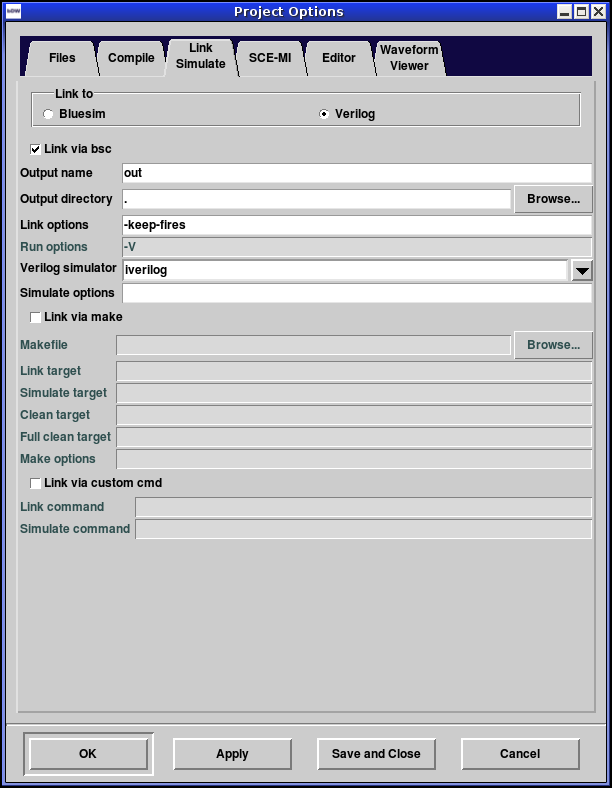
\includegraphics[width = 3 in]{figures/options-link}
\caption{Project Options - Link}
\label{fig-link}
\end{center}
\end{figure}

\paragraph{Link via bsc}
\index{bsc}
Linking via bsc runs the Bluespec compiler again to link the compiled
hardware description into the simulation environment,  Bluesim or
Verilog,  as determined  by the option set on
the top of the  tab.  On the {\bf Link/Simulate} tab you  specify the
following fields:
\begin{itemize}
\item  the name of the output file
\item output directory
\item  linking flags
\end{itemize}

When left blank, the output directory defaults to the current
working directory.   The output file name and output directory are
passed to the \te{bsc} command with the \te{-o} flag.  The following
table lists the field on the {\bf Link/Simulate} tab and the associated bsc
compiler flags.

\begin{center}
\begin{tabular}{|p{1 in}|p{1 in}|p {3 in}|}
\hline
{\bf Field} &{\bf Compiler flag}&{\bf Description}\\
\hline
\hline
Bluesim & -sim & Compiles for Bluesim\\
\hline
Verilog & -verilog&Compiles for Verilog\\
\hline
Output name& -o& Name for the binary being created; the default name
is \te{a.out}\\
\hline
Link options & bsc flags & See BSC documentation\\
\hline
Simulator&-vsim&Specifies which Verilog simulator to use\\
\hline
\end{tabular}
\end{center}



\paragraph{Simulate}
\index{simulate options}
\index{settings!simulate options}
\label{options-simulator}

\index{-V@\te{-V}}
If
compiling to Bluesim, you can specify Bluesim run options, such as the \te{-V}
flag to generate VCD files, in the Simulate options field.

If the {\bf Compile to} target is Verilog, the following simulators can be
chosen in the {\bf Link/Simulate} tab:
\begin{itemize}
\item \te{iverilog}
\item \te{modelsim}
\item \te{ncverilog}
\item \te{vcs/vcsi}
\item \te{cver/cvc}
\item \te{veriwell}
\item \te{isim}
\end{itemize}

\index{+bscvcd@\te{+bscvcd} (Verilog simulation)}
When using any of the above simulators, use the Simulate options field
to specify the simulation plusarg variable \te{+bscvcd},
as described in Section~\ref{simulate}.


\paragraph{Link via make}
\index{makefile!using}
The fields on the {\bf Link/Simulate} tab for  {\bf Link via make}
are as follows:
\begin{itemize}
\item Makefile
\item Target
\item Simulation Target
\item Clean Target
\item Options
\end{itemize}

\index{meta variable}


You can  use Unix environment variables and the Workstation meta
variables (Section \ref{metavariable}) in the makefile fields.

\paragraph{Linking via custom command}

You can use other simulation environments, by supplying the Link
command and the  command to launch  the
simulator (Simulate Command).
  This allows you to link the design with any simulation environment you choose.

\index{meta variables}

You can  use Unix environment variables and the Workstation meta
variables (Section \ref{metavariable}) in the link and simulate
command fields.

% -----

\subsubsection{Editor}
\index{editor options}
\index{settings!editor options}
\index{emacs}
\index{gvim}

\begin{figure}[ht]
\begin{center}
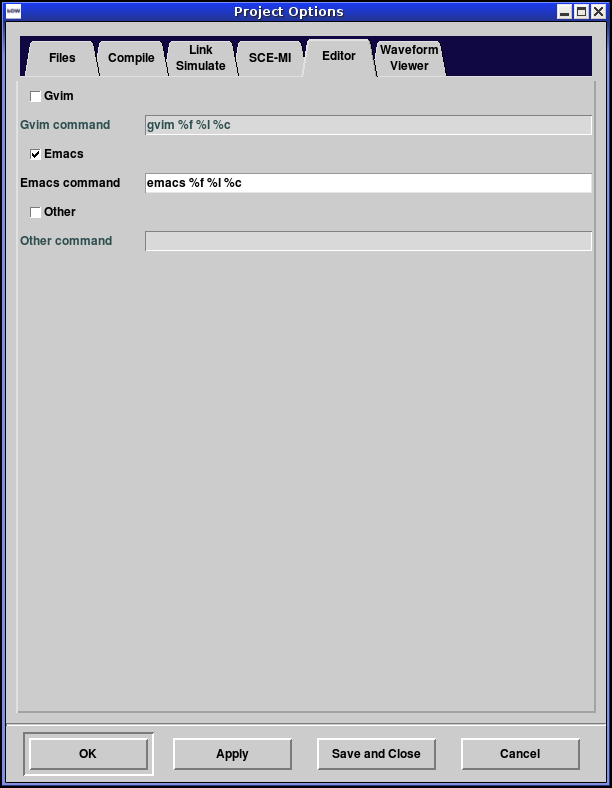
\includegraphics[width = 3 in]{figures/options-editor}
\caption{Project Options - Editor}
\label{fig-editor}
\end{center}
\end{figure}

The editor is selected in the {\bf Editor} tab, as shown in Figure
\ref{fig-editor}.   The supported editors are  \te{gvim}  and
\te{emacs}.   The selected
editor is used whenever files are opened within the
Development Workstation. Bluespec editing modes for these editors are
provided with BSC.

% -----

\subsubsection{Waveform Viewer}
\index{waveform viewer!options}
\index{waveform viewer!SpringSoft/Novas}
\index{waveform viewer!GtkWave}
%\index{waveform viewer!Mentor}
\index{settings!waveform viewer options}
\index{SpringSoft/Novas}
\index{GtkWave}
%\index{Mentor
\label{options-waveform}


\begin{figure}[ht]
\begin{center}
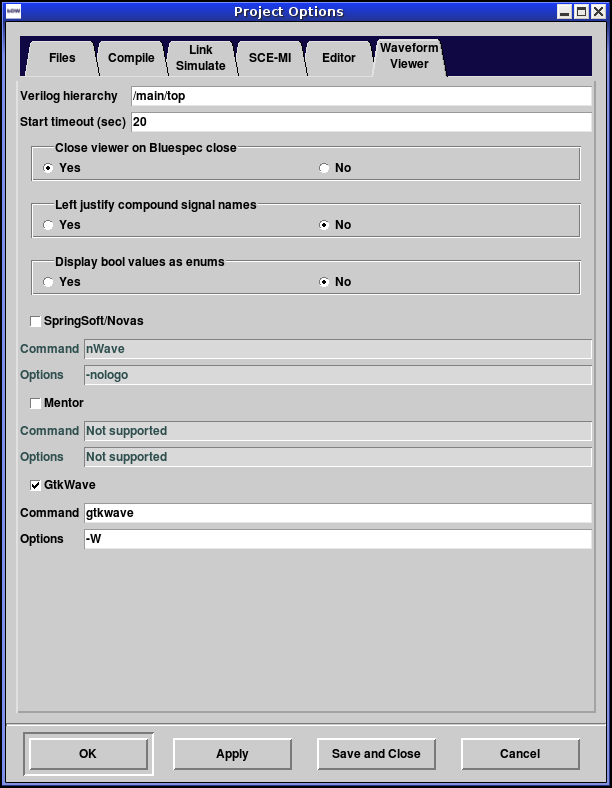
\includegraphics[width = 3 in]{figures/options-wave}
\caption{Project Options - Waveform Viewer}
\label{fig-wave}
\end{center}
\end{figure}

The Development Workstation can interface to the waveform viewers
provided by SpringSoft/Novas (Verdi, Debussy, nWave) and GtkWave.  % and Mentor.
The {\bf Waveform Viewer} tab, as shown in
Figure \ref{fig-wave},   is where you enter the command for
   launching the waveform viewer along with any
 command line options.  This is  also where you  specify the viewer timeout
value and control how compound signal names will be displayed.
 Generating waveforms from Bluesim and Verilog
simulators is discussed in  Section \ref{simulate}.

To use GtkWave with the Development Workstation requires release 3.3 or later of GtkWave.
The \te{-W} flag must be specified in the {\bf Options} field  under
the command of \te{gtkwave}.  To build GtkWave, Tcl/Tk must be
installed.  

% -------------------------

\subsection{Editing Files with the Project Files Window}
\index{options!files}
\label{project-window}

The {\bf Project Files} window is the primary window for viewing,
editing, and compiling individual design files.  When you open a project, the
Workstation opens the {\bf Project Files}  window displaying  all the
files  meeting the criteria specified in the {\bf Files} option tab.  By default, all
\te{.bsv} files in the project search path  are listed.



% \begin{figure}[ht]
% \begin{center}
% \subfigure[Project Files Window1]{\label{fig1}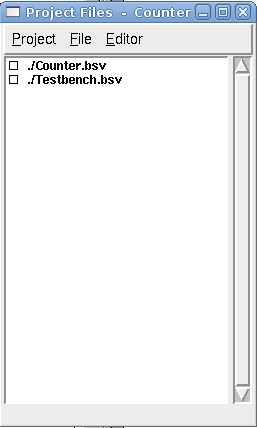
\includegraphics[height = 2.4 in]{figures/projectfiles1}}
% \subfigure[Project Files Window2]
% {\label{fig2}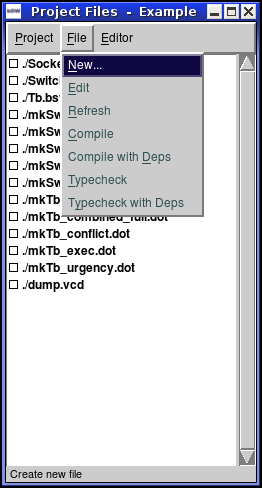
\includegraphics[height = 2.4 in]{figures/projectfiles_menu}}\\
% \end{center}
% \caption{Project Files Window}
% \label{fig-projectfiles2}
% \end{figure}

\begin{figure}[ht]
\begin{center}
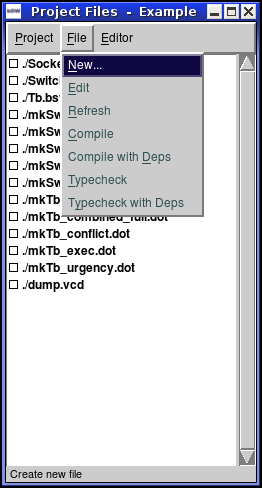
\includegraphics[height = 2.4 in]{figures/projectfiles_menu}
\caption{Project Files Window}
\label{fig-projectfiles}
\end{center}
\end{figure}


To edit a file from the {\bf Project Files}
window, you can either
double-click on the file, or select the file and then  {\bf
File$\rightarrow$Edit}, as shown in Figure \ref{fig-projectfiles}.
The editor  set in the {\bf Editor} option tab
(gvim or emacs) will be used.

You can also create a new file from the {\bf Project Files} window.
Select {\bf File$\rightarrow$New} and a new file will open in the text editor.

Within this window you can  compile individual files or entire projects.  Section~\ref{sec-compile}
describes the compile process.  You can execute an action (edit,
refresh, type check,
compile) on a file by selecting the file and then
either using the context menu to select an action or the {\bf File}
pull-down menu.

To change the files displayed, editor used, or any of the other project options, use the {\bf
Project$\rightarrow$Options} menu.
See Section~\ref{project-options} for a complete description of the
Project Options and how to modify them.

% -------------------------

%\subsection{Editing a Project}

% -------------------------

\subsection{Saving a Project}
\index{save}

When you save a project, either through the {\bf Save} or {\bf Save
As} options on the {\bf Project} menu, you are saving the options
defined on the {\bf Project Options} tabs.

%\subsubsection{Saving Window Placement}
\index{window placement}
\index{save placement}

% The Development Workstation consists of multiple windows, many of
% which  may be open at the same time.
You can save the relative placement
of the windows by selecting {\bf Save Placement} on the {\bf Project}
menu.  The placement is only saved through the {\bf Save Placement}
option, it is not saved when saving a project.

% -------------------------

\subsection{Maintaining  Multiple Settings for a Single Design}

A single design may have multiple sets of options or settings. For example, you
may want to generate both Bluesim and Verilog targets from a single
design, or save both test and production settings, or use different
versions of library files.  In each case you will have a unique set of
options;  each set is  saved in its own project (\te{.bspec}) file.

 The
following example describes some the  settings for  generating both Bluesim
and Verilog from a single set of \te{.bsv} files.

\begin{itemize}
\item Each target is  its own project, defined by its own
\te{.bspec} file.
\item The  same  \te{.bsv}
files are used in  both projects therefore the project directories  are the same.
\item In the {\bf Project Options}  the following fields are different:
\begin{itemize}
\item In the {\bf Files} tab different output directories are
specified for each project so  the generated files are not
overwritten when the other target is compiled.  All output files
(Bluesim or Verilog, \te{.bo/.ba}, Info files)  have
different  directories specified for each  project.
\item In the {\bf Compile} tab, the target is set to  Bluesim in one
project,  and Verilog in the other.
\item Also in the {\bf Compile} tab different compiler flags may be
used for each target.
\end{itemize}
\item In the {\bf Link/Simulate} tab,  different output directories are
specified and well as link compiler options for each project.
\item Also in the {\bf Link/Simulate} tab different simulators are
specified along with  any  options for the simulator.
\end{itemize}

  The Development Workstation project saves each group of
settings and options in the \te{.bspec} file, allowing you to maintain multiple
design environments for single set of \te{.bsv} files.

% ------------------------------------------------------------
% Section: Building a Project

\section{Building a Project}
\index{build}
\label{build}

Building a project includes running the compiler and simulating designs.
 All build options are  available from the {\bf Build} menu and on the  toolbar, as shown in
Figure \ref{fig-toolbar}.  Additional build options include stopping
  active processes and removing
 generated files (\te{Clean} and
\te{Full Clean}).  Some  options combine multiple build actions into single
 option or button, for example,  \te{Compile + Link}.

\begin{figure}[ht]
\begin{center}
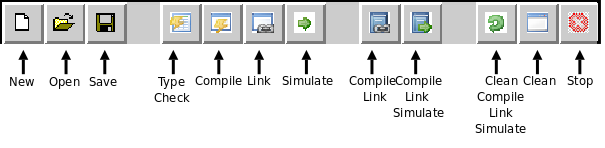
\includegraphics[width = 5.5 in]{figures/toolbar1}
\caption{Workstation Toolbar}
\label{fig-toolbar}
\end{center}
\end{figure}

% -------------------------

\subsection{Type Check}
\label{sec-type check}
\index{type check}
\index{.bo@\te{.bo}}

There are two stages in  compilation, type checking and
code generation, executed by a single compile command.
The simplest compilation of a BSV design is to run only the first
stage of the compiler which is the {\bf Type Check} task, generating
the \te{.bo} files.   Once the type check is
 complete, you have enough module
information to  use the {\bf Package}  and the {\bf Type Browser} windows.
When you select the {\bf Type Check} task, the compiler stops before
code generation, even if there are no errors in the compile.

A BSV design  often imports other packages.  The
Development Workstation will automatically type check those packages, if necessary,
when you type check  a project. When type checking an individual file you
must specify {\bf type check with deps} if you want to type check the imported
packages.   Section~\ref{sec-import-packages}
discusses importing packages in more detail.

% -------------------------

\subsection{Compile}
\label{sec-compile}
\index{compile}
\index{.bo@\te{.bo}}
\index{.ba@\te{.ba}}
\index{.v@\te{.v}}
\index{Verilog}

The {\bf Compile} task runs the full compilation including both the
type checking and code generation stages.  The first stage (type
check) generates the \te{.bo} file.
The second stage (code generation) generates an elaborated module file
(\te{.ba}) and, when the target is Verilog, a (\te{.v})  file.  These
generated files have the same name as the module they implement, not
the name of the package or file they come from.


\index{attributes!synthesize}
\index{synthesize attribute@\te{synthesize} attribute}
\index{-g@\te{-g} (compiler flag)}
\index{top module}
To run the compiler through to code generation, a  module must be marked
for synthesis.  The recommended method is to use  the
\te{synthesize} attribute in the BSV code.  You can also  specify a
top  module in the {\bf Project Options$\rightarrow$Files} tab, which is the same as
passing the top module with the \te{-g} compiler flag.  See Section~\ref{spec-code-gen} and the
The BSV  Reference Guide for information on  synthesizable modules.

\index{import packages}
A  package  often imports other packages.  The
Development Workstation will automatically recompile imported packages, if necessary,
when you compile  a project. This is the same as specifying the
\te{-u} option on the command line.  When compiling an individual file you
must specify {\bf compile with deps} if you want to recompile imported
packages.   Section~\ref{sec-import-packages}
discusses importing packages. Section~\ref{sep-compile} contains
 a detailed explanation of  techniques and considerations
when  compiling a collection of BSV modules.

The compiler  automatically runs through to code generation if no
errors are  encountered in the type checking stage and a module is
marked for synthesis.  If errors are encountered in the type check
stage,  the compiler will halt before generating the
\te{.bo} file. In this case the {\bf Package} and {\bf Type
Browser} windows will not be able to display the project specific
packages, as they depend on these
intermediate files. If errors are encountered in the second stage, the
\te{.bo} file will be created but the \te{.ba} file will not.
In this case the {\bf Module Browser}, {\bf Schedule Analysis}, and
{\bf Scheduling Graphs} windows will not display project-specific
packages.  BSC-provided library packages can always be viewed in
the Workstation, since the \te{.bo} files for these packages are
always available.

\index{-sched-dot@\te{-sched-dot} (compiler flag)}
To view the scheduling graphs the compiler flag \te{-sched-dot} must be
specified for compilation, in the {\bf Project
Options$\rightarrow$Compile} tab.  This flag generates the \te{.dot} files
from which the graphs are generated.

% \begin{figure}[ht]
% \begin{center}
% 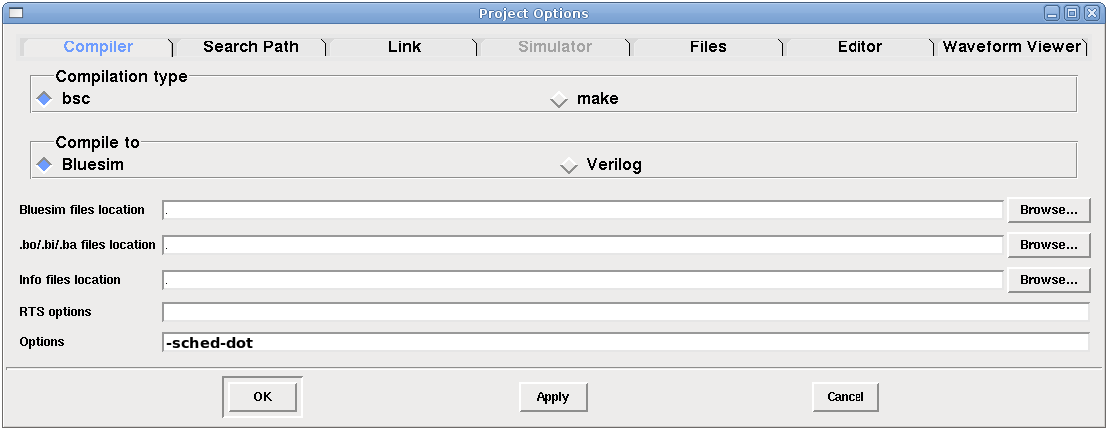
\includegraphics[width = 5 in]{figures/compileroption-scheddot.png}
% \caption{Options - Compiler with -sched-dot flag}
% \label{fig-sched-dot}
% \end{center}
% \end{figure}

% -----

\subsubsection{Compiling a File}

A project  usually contains  multiple packages and files.
To compile a single file, use the {\bf Project Files} window.  Select
the file to be compiled and then {\bf Compile}, from either the {\bf File}
pull-down menu or the context menu.

\paragraph{Compiling with dependencies}
\index{compile with deps}
Compiling with dependencies means that you want to compile any
imported files, if necessary, before compiling the selected file.
This is equivalent to compiling with the \te{-u} flag.  The
compiler compares the time stamp on the \te{.bo} file
to determine if the imported file has changed since the last
compilation.  When you compile with dependencies  only changed files
will be recompiled.
You can choose {\bf Compile with Deps} from both the {\bf File} and the
context menus.

% \index{compiler messages}
% You may see different messages in the main window when you compile
% with dependencies and when  compile without
% dependencies.  In the compiling with dependencies case, only changed
% files will be recompiled.  If the selected file has not changed since
% the last compile, it won't be recompiled, so you won't see previous
% error messages or warnings.

% -----

\subsubsection{Compiling a Project}
\index{top file}
\index{synthesize attribute@\te{synthesize} attribute}
\index{attributes!synthesize}

You can compile your complete project from the toolbar, the {\bf Build}  menu or the
{\bf Project Files} window. Before compiling,  the file to be compiled
must be specified in the {\bf\tt top file} field on the {\bf Files} option
tab.

  The \te{top module} is not required for compiling,
but is required for linking.  If the  \te{top module} is not
specified, the \te{synthesize} attribute must be used in the BSV code
to compile through code generation.  Otherwise, the project will only
be compiled through elaboration, generating the \te{.bo} file, but
not the \te{.ba} file.  Specifying the \te{top module} in the {\bf Files}
tab is equivalent to using the \te{-g} flag with the name of the
 module.

% \begin{figure}[ht]
% \begin{center}
% 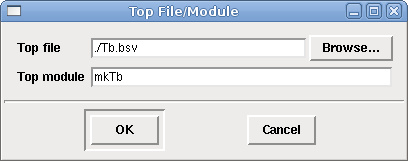
\includegraphics[width = 2 in]{figures/topfile}
% \caption{Top File Menu}
% \label{fig-topfile}
% \end{center}
% \end{figure}


 When compiling a project from the Development Workstation the \te{-u}
 flag is  always used;  timestamps on all imported
files are checked and files are recompiled as necessary.

% -----

%\subsection{Understanding Compilation}

\subsubsection{Specifying modules for code generation}
\label{spec-code-gen}
\index{selecting modules}
\index{code generation}
\index{-g@\te{-g} (compiler flag)}
\index{synthesize (attribute)}

A module can be selected for code generation either in the BSV code or
at compile-time.  The recommended method is to mark the module for
code generation in the BSV code, using the \te{synthesize} attribute
(see the BSV Reference Guide for more information on
attributes).  The alternative is, at compile-time, to use the {\bf Top
Module} field  which  instructs the compiler to generate code for a
particular module.  This is the same as using the  {\bf\tt
-g} flag on the Unix command line with the \te{bsc} command, From the
command line, the {\bf\tt -g} flag can be used multiple times
within a compile
 command line to specify multiple modules for code generation.

Whether the generated  code will be Bluesim or Verilog depends on
which back end has been selected, either through the {\bf Options} window or
by using  the  {\bf\tt -verilog} or
{\bf\tt -sim}  command line flag.
\index{-sim@\te{-sim} (compiler flag)}
\index{-verilog@\te{-verilog} (compiler flag)}

If none of the  modules are marked for
synthesis, the compiler will not generate a hardware description (a
Verilog {\bf\tt .v} file  or a Bluesim {\bf\tt .ba} file).

Not all modules written in BSV are synthesizable.

% -----

\subsubsection{Importing other packages}
\index{importing packages}
\label{sec-import-packages}
\index{library packages}

To compile a package that imports another package,
BSC needs the \te{.bo} file from the imported
package.  One way to provide this file is to run the compiler on
each imported file. Or the Development Workstation
will automatically determine which files are needed and recompile as
necessary, when compiling a project.
If the \te{.bo} file already exists, the compiler will
only recompile if the file has changed since the last compilation, as indicated
by the imported file having a more recent date than the file being compiled.

For example, to compile  a package {\bf\tt Foo} that imports another package
{\bf\tt Baz}, BSC needs to examine the file {\bf\tt Baz.bo}. If {\bf\tt Baz} is in the file {\bf\tt
Baz.bsv},  then this file needs to be run
through the compiler to produce the necessary  {\bf\tt
.bo} file before the compiler can be invoked on {\bf\tt Foo.bsv}.  If
in the Workstation you
 compile a project or compile a file with dependencies, or if you  use
 the {\bf\tt -u} flag on the command line, the compiler will check to see if
 {\bf\tt Baz.bo} exists, and if it exists, it will
check the compilation date.  The compiler will recompile the {\bf\tt
Baz} file if necessary.

BSC comes with a set of library files providing common
and useful hardware structures, such as
\te{FIFO} and \te{UInt}.  They are  described in the BSC
documentation.   The source code for these packages is already
compiled and the  \te{.bo} files are
found in a library directory with the compiler installation (in
the same way that C header and object files are stored in standard
\emph{include} and \emph{library} directories). The compiler looks for
these files in:

\begin{centerboxverbatim}
%/Libraries/
\end{centerboxverbatim}
The BSC \te{Libraries} directory is automatically
added to the search path  when a project is created in  the Workstation.

If you are importing packages from other directories, the
directories must be added to the search path.  In the Workstation
use the {\bf Files} tab on the {\bf Options} menu, as described in
Section~\ref{options-searchpath}, to modify the path.

% BSC also comes with a set of library files for which both the BSV
% source is provided in the \te{BSVSource} directory,
% along with compiled \te{.bo} files in the
% \te{Libraries} directory.  You can use these packages as provided, or
% edit and customize them
% to your own specifications.  To use a customized version of the these
% files, include the directory containing the \te{.bsv} source files in the search
% path. If the directory containing the  \te{.bsv} files  is in any
% position in the search path, the modified \te{.bsv} will be used, and not
% the precompiled \te{.bo} files from the \te{Libraries} directory.

% -----

\subsubsection{Understanding separate compilation}
\label{sep-compile}
\index{compilation}

BSC has two main stages; first it converts BSV modules
into a collection of states and rules, and then it converts the
rule-representation into a hardware description.

When compiling a collection of BSV modules, it is up to the user to
decide which of these modules should be compiled to hardware
separately, and which should be subsumed into the parent module.  By
default, all hierarchy is flattened into one top-level module in the
final hardware description, but the user can specify   modules which should
stay in the hierarchy and
have separate hardware descriptions.

 What happens when
a module {\bf\tt m1} instantiates another module {\bf\tt m2}?
If the submodule {\bf\tt m2} is provided as a BSV
description, that description will need to be compiled into a set of
rules and then those rules combined with the rules for {\bf\tt m1} to
be converted, by the code generation stage, into a  hardware
description.

If {\bf\tt m2} is provided as a hardware
description (that is, implemented in a Verilog file or in Bluesim header and
object files), then the hardware description for {\bf\tt m1} will
contain an instantiation of {\bf\tt m2}.  The implementation of
{\bf\tt m2} is kept in its own file.
For the Verilog back end, this produces a {\bf\tt m1.v}
file with a Verilog module {\bf\tt m1} which instantiates {\bf\tt m2}
by name and connects to its ports but doesn't contain the
implementation of {\bf\tt m2}. Both implementation files, {\bf\tt
m1.v} and {\bf\tt m2.v}, must be provided to the simulation or
synthesis tools.

\index{synthesize (attribute)}
\index{-g@\te{-g} (compiler flag)}

Even if {\bf\tt m2} is provided as a BSV description, the user can
decide to generate a separate hardware description for the module.
This is done by putting the \te{synthesize} attribute in the BSV
description   or using the
{\bf\tt -g} flag, indicating that
 the module should be synthesized
as a separate module, apart from the instantiating module.

\index{.bo@\te{.bo} (file type)}
 The
implementation in a {\bf\tt .bo} reflects whether hardware was
generated for a module.  If a hardware description was generated for a
module, then the implementation in the {\bf\tt .bo} will be merely a
pointer to the location of that description (be it {\bf\tt .v} or
{\bf\tt .o}). If hardware was not generated for the module, then an
entirely BSV representation will be stored in the {\bf\tt .bo} file.

Thus, a single {\bf\tt .bsv} file can be compiled in different ways to
produce very different {\bf\tt .bo} files.  When the
compiler is generating hardware for another BSV file that imports this
package, it will need to read in the information in the {\bf\tt .bo}
file. How it is compiled depends on the flags used. Therefore, compiling the
new file will be affected by how the imported file was compiled earlier!  It
is important, therefore, to remove these automatically generated files
before beginning a new compilation project, especially if a different
module hierarchy is desired.

For example, if a user were to generate Verilog for a module {\bf\tt mkFoo}
just for testing purposes, the {\bf\tt Foo.bo} would encapsulate into its
own description the information that a Verilog module had been generated
for module {\bf\tt mkFoo}.  If the user then wanted to generate Verilog for a
larger design, which included this module, but wanted the larger design
to be compiled into one, hierarchy-free Verilog module, then the {\bf\tt .bo} file would
have to be deleted so that a new version could be created that only
contained the state-and-rules description of the module.

When using the Development Workstation the {\bf Clean} tasks (Section~\ref{clean}) will remove these files.
The {\bf Clean} task removes the \te{.bo} files, while the {\bf Real
Clean} task removes the generated Verilog (\te{.v}) files as well.

% -----

\subsubsection{Interfacing to foreign modules and functions}
\index{importing foreign functions}
Foreign modules and functions can be included as part of a BSV model.
A designer can specify that the implementation of a particular BSV
module is provided as either a Verilog module or a C function.

% -----

\subsubsubsection{Importing Verilog modules}
\index{import BVI}
\index{importing Verilog}
\index{Verilog!importing}

Using the \te{import "BVI"} syntax, a designer can
specify that the implementation of a particular BSV module is an RTL
(Verilog or VHDL) module, as described in the BSV  Reference Guide.
The module is treated exactly as if it were originally
written in BSV and then converted to hardware by the compiler,  but
instead of the {\bf\tt .v} file
being generated by  the compiler, it was
supplied independently of any BSV code. It may have been written by
hand or supplied by a vendor as an IP, etc. The files for these
modules need to be linked in to the simulation.

TBD -- What needs to be specified in the Workstation?

% Several primitive BSV elements, such as FIFOs and register files, are
% expressed this way --- as Verilog primitives.  When simulating or
% synthesizing a design generated with the Verilog back end, you will
% need to include the appropriate hardware descriptions
% for these primitives. Verilog descriptions for BSC-provided
% primitive elements can be found in:
%
% \begin{centerboxverbatim}
% ${BLUESPECDIR}/Verilog/
% \end{centerboxverbatim}

% -----

\subsubsubsection{Importing C functions}
\index{import BDPI}
\index{importing C}

Using the importBDPI syntax, the user can specify that the
implementation of a BSV function is provided as a C function.
The same implementation can be used when simulating with Bluesim or
with Verilog.  In Bluesim, the imported functions are called directly.
In Verilog, the functions are accessed via the Verilog VPI. \index{Verilog Procedural Interface (VPI)}

TBD -- What needs to be specified in the Workstation?

If the foreign function uses any
system libraries, or is itself a system function, then the linking stage
will need to include those libraries.  This is done on  the
{\bf Project Options$\rightarrow$Files} tab in the Workstation.
% From
% the command line  the user can specify libraries to
% include with the {\bf\tt -l} flag and can specify non-default paths to
% the libraries with the {\bf\tt -L} flag.

% -------------------------

\subsection{Link}
\label{linking}
\index{linking}
\index{link}

The compiled  hardware description  must be linked into a simulation
environment before you can simulate the project.  The result of the linking
stage is a binary which, when executed,
simulates a module.
BSC required for linking \index{Bluesim} Bluesim generated modules and can
be used to link Verilog\index{Verilog} modules as well.
% generated  modules can be handled as you would any other Verilog
% modules.  They can be linked via BSC
To link in the Workstation, select {\bf Link} from the toolbar or the
{\bf Build} menu.

The simulation environment and location of the implementation files are
specified in the  {\bf Files} tab of the {\bf Options} menu.
The top-level module must also be specified in {\bf Files} tab of the
the  {\bf Options} menu.
You can specify additional link compiler flags
in the {\bf Link/Simulate} tab of the {\bf Options} menu.

If you've compiled your design and you still cannot link (the {\bf
Link} option is grayed out), the design is  not ready to be
linked.  To determine the cause, you should verify that:
\begin{itemize}
\item  The compile completed successfully and \te{.ba}
files were generated for  the \te{.bsv} files.
\item  A {\bf top module} is specified in the {\bf
Project Options} menu, {\bf Files} tab.
\end{itemize}

% -----

\subsubsection{Linking with Bluesim}
\index{Bluesim back end}
\index{Bluesim!linking .ba files}

For the Bluesim back end, linking means incorporating a set of Bluesim object
files that implement BSV modules into a Bluesim simulation
environment.
Bluesim is specified in the {\bf Project Options} window
or by using the {\bf\tt -sim} flag.
% In an installation of the BSV
% compiler, the  files for
% this simulation environment are stored with the other Bluesim files
% at: \verb|${BLUESPECDIR}/Bluesim/|.

TBD -- Include paths, files, libraries, etc for linking?

% -----

\subsubsection{Linking with Verilog}
\index{Verilog back end}
\index{Verilog!linking}
\index{Verilog!simulator}

For the Verilog back end, linking means invoking a Verilog compiler to create a
simulator binary file or a script to execute and run the
simulation.
The Verilog simulator is specified in the {\bf Project
Options$\rightarrow$Link/Simulate} tab or by  using the {\bf\tt
-vsim} flag.

\index{Verilog simulator!vcsi}
\index{Verilog simulator!vcs}
\index{Verilog simulator!ncverilog}
\index{Verilog simulator!modelsim}
\index{Verilog simulator!cver}
\index{Verilog simulator!veriwell}
\index{Verilog simulator!iverilog}
\index{Verilog simulator!isim}
\index{vcsi (Verilog simulator)}
\index{vcs (Verilog simulator)}
\index{ncverilog (Verilog simulator)}
\index{modelsim (Verilog simulator)}
\index{cver (Verilog simulator)}
\index{veriwell (Verilog simulator)}
\index{iverilog (Verilog simulator)}
\index{isim (Verilog simulator)}
\index{-vsim@\te{-vsim} (compiler flag)}

\label{sec:using-verilog}
The {\bf Link/Simulate} tab and the \textbf{\texttt{-vsim}} flag
(along with the equivalent
\textbf{\texttt{BSC\_VERILOG\_SIM}} environment variable) govern which Verilog
simulator is employed; at present, natively supported choices for
\textbf{\texttt{-vsim}} are \texttt{vcs}, \texttt{vcsi}, \texttt{ncverilog},
\texttt{modelsim}, \texttt{cver(cvc)},  \texttt{iverilog},
\texttt{veriwell}, and \texttt{isim}.  If the simulator is not specified \texttt{bsc} will attempt to detect one
of the above simulators and use it.

When the argument to \textbf{\texttt{-vsim}} contains the slash character
(\texttt{/}), then the argument is interpreted as the name of a script to run
to create the simulator binary.  Indeed, the predefined simulator names listed
above refer to scripts in the BSC distribution; thus,
\texttt{-vsim vcs} is equivalent to \texttt{-vsim
\$BLUESPECDIR/lib/exec/bsc\_build\_vsim\_vcs}.  The simulator scripts distributed
with BSC are good starting points should the need to use an unsupported
simulator arise.

To add  directories to the search path when linking Verilog designs,
use the \te{-vsearch}\index{-vsearch@\te{-vsearch} (compiler flag)} flag.
For example, adding the flag \te{-vsearch
+:verilog\_libs} to the {\bf Link Options} field will add the directory
\te{verilog\_libs} to the simulator search path (for simulators such
as \te{iverilog} and \te{vcs/vcsi}).  This is equivalent to adding \te{-y
<directory>} to the Verilog compilation command.

The generated Verilog can be put into a larger Verilog design, or run
through any existing Verilog tools.  BSC also provides a
convenient way to link the generated Verilog into a simulation using  a
top-level module (\te{main.v}) to provide a clock for the design.  The
BSC-provided \te{main.v} module instantiates the top module
and toggles the clock every five simulation time units.
The default \te{main.v} is the default  used when running a Verilog simulation in
the Development Workstation.
From the command line the following
command  generates a simulation binary \te{mkFoo.exe}:

\begin{centerboxverbatim}
bsc -verilog -e mkFoo -o mkFoo.exe
\end{centerboxverbatim}

With this command the top level Verilog module \te{main} is taken from
\te{main.v}.  \te{main.v} provides a clock and a reset, and
instantiates \te{mkFoo}, which should provide an \te{Empty}
interface.  An executable file, \te{mkFoo.exe} is created.

% -------------------------

\subsection{Simulate}
\label{simulate}
\index{FSDB}
\index{VCD}

The {\bf Simulate} task runs the simulation executable generated by the linking
task, using the simulator and options specified in the {\bf Options}
window.  The results are displayed in the status/log window.

To view waveforms, you must generate a waveform dump file, either VCD
 or FSDB, during simulation.


You can generate a VCD file from either Bluesim or any of the
 supported Verilog simulators.  When simulating with Bluesim, use
 the \te{-V} flag.   For Verilog simulators using
the BSC-provided \te{main.v} file, specify the \te{+bscvcd} flag during
simulation.   Simulation flags are entered in the options field of the
 {\bf Project Options$\rightarrow$Link/Simulate} window, as described
 in
Section \ref{options-simulator}.


To dump a FSDB file directly from a supported Verilog simulator using
the BSC-provided \te{main.v} file, you  need to specify the
\te{+bscvcd} flag during simulation and the  \te{-D BSV\_FSDB} flag
during linking.   Note
that not all simulators can generate an FSDB file. Additional command
line arguments are required, dependent on the simulator. The FSDB
libraries  from Novas/SpringSoft must also be linked in.
 Bluesim does not
generate FSDB files at this time.

% -------------------------

% \subsection{Full Rebuild}

% The {\bf Full Rebuild} task combines the following build steps:
% \begin{enumerate}
% \item Full Clean
% \item Compile
% \item Link
% \item Simulate
% \end{enumerate}

% -------------------------

\subsection{Stop}

To stop a build process before completion, use the {\bf Stop} option.  It
stops the running compile, link or simulation by sending a kill to the process
and any subprocesses.

% -------------------------

\subsection{Clean and Full Clean}
\index{clean}
\index{full clean}
\label{clean}

There are two
options to clean your files: {\bf Clean} and {\bf Full Clean}.  {\bf
Clean} removes the intermediate files generated during compilation: the
\te{.bo}, \te{.ba}, and \te{.o} files.
Before recompiling, you may want to
remove the intermediate files to force the compiler to recompile
all  imported packages.
{\bf Full Clean} removes all generated result files - \te{.sched},
\te{.v}, \te{.so}, and \te{.exe} -  in addition to
the intermediate compilation files.

\index{makefile!using}
If you are compiling via a  makefile,
then both {\bf Clean} and {\bf Full Clean}  will instead execute the
appropriate target in the makefile, as specified in the {\bf Compile}
and {\bf Link/Simulate} tabs of the {\bf Project$\rightarrow$Options} window.

% ------------------------------------------------------------
% Section: Analyzing a Project

\section {Analyzing a Project}

The design browsers within the Development
Workstation provide different views of the design.
The following table summarizes the
windows and browsers in the Development Workstation.

%  Which window or browser you use for a given
% task depends on the information you want to see and the stage of the
% design.  The {\bf Project Files} window lists the \te{.bsv} files
% in the project and is always available.  As soon as a project
% has been  created, \te{.bsv} files can be
% created, viewed,  edited, and compiled from  this window.   The
% {\bf Package}  and {\bf Type Browser} windows provide a high-level
% view of the package and type hierarchies within the design.  These viewers
%  require the first stage of compilation, pre-elaboration, to complete.   The  {\bf
% Module Browser} and  {\bf Schedule Analysis} windows are used only
% after the full compilation,
% through to code generation  has
% completed.  From the {\bf Schedule Analysis} window you can link to a waveform viewer where you
% can view Bluespec type and structure information along with the waveforms.

% \index{.bi/.bo@\te{.bi/.bo}}
% \index{.ba@\te{.ba}}
% The information needed to display package and type information is
% stored in the intermediate \te{.bi/.bo} files, created during the
% first part of the compilation, parsing and type checking.  Complete rules, method calls and
% schedule information is stored in the \te{.ba} files.

\begin{center}
\begin{tabular}{|p {1.7 in}|p {3.2 in}|p {.5 in}|}
\hline
\multicolumn{3}{|c|}{BSC Development Workstation Windows}\\
\hline
Window&Function&Required \\
&&Files\\
\hline
\hline
Main Window&Central control window.   Manage projects, set project
options, build projects, and monitor status. &\te{.bspec}\\
\hline
Project Files Window&View, edit and compile files in the
project.& \te{.bsv}\\
\hline
Package Window&Pre-elaboration viewer for the design.   Load
packages into the Development Workstation and browse their contents.  Provides a
high-level view of the types, interfaces, functions and modules
defined in the package.&\te{.bo}\\
\hline
Type Browser&Primary means for viewing information about types and
interfaces.  Displays the full structure hierarchy and all the
concrete types derived from resolution of polymorphic types.&\te{.bo}\\
\hline
Module Browser&Post-elaboration module viewer, including rules and
method calls.  Displays the design hierarchy and an overview
of the contents of each module. Provides an interface to the waveform
viewer.&\te{.ba}\\
\hline
Schedule Analysis Window&View schedule information including warnings,
method calls, and conflicts between rules for a module.&\te{.ba} \\
\hline
Scheduling Graphs&  Graphical view of schedules, conflicts, and
dependencies.&\te{.ba  .dot}\\
\hline
\end{tabular}
\end{center}

% -------------------------

\subsection{Viewing Packages with the Package Window}

\label{window-package}
\index{package}
\index{import}

The {\bf Package} window provides a high-level view of the contents of
the project, sorted by package.  You can perform the following tasks in the {\bf Package} window:
\begin{itemize}
\item View a complete list of packages.
\item View the import hierarchy of a selected package.
\item View the contents of each package.
\item View basic information on types, interfaces, functions, and modules.
\item Navigate to the {\bf Type Browser} for a particular type.
\item Open and edit  source code.
\item Search types and functions for a string or a regular expression.
\end{itemize}

\begin{figure}[ht]
\begin{center}
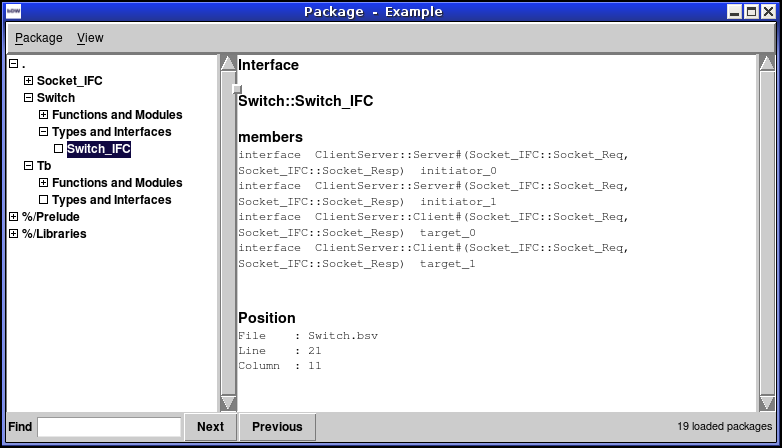
\includegraphics[width = 5 in]{figures/package}
\caption{Package Window}
\label{fig-package}
\end{center}
\end{figure}


The {\bf Package} window, shown in Figure \ref{fig-package},  has two panes.  The left pane lists  packages
 by directory; the right pane displays the definition of  a selected object.
To view a package or any object within it, the package
must first be loaded ({\bf Package$\rightarrow$Load}) into the Development Workstation.  When you load a package, all packages imported by that
package are loaded along with it.  Therefore, if you load the
 \index{top package} top package  ({\bf Package$\rightarrow$Load Top
 Package}),  all packages used by the project will be loaded.
The  \te{Prelude} package is automatically imported in every BSV design and  will
 be loaded along with the first package you load.    If you don't see a specific
package in the left pane, it has not been loaded yet.

The {\bf Package} window will only display packages which have
\te{.bo} files.
Since library files (BSC-provided files in the
\%/Libraries directory) are precompiled, these are always
available, even before compiling the project.  Project specific files have to  be compiled through
type checking (\te{.bo} files) to view them in the {\bf Package} window.



Click on the icon next to
the package name to expand and view the
types, interfaces, functions and modules defined in the package.
Click on the name of  any item  in the   package
to view its definition in the right pane.  The {\bf Package} window can be helpful in displaying the
functions defined in a package, especially for packages such as
\te{Vector} which contain many functions.

The amount of information
displayed for each item type is
limited and detailed information is only available for leaf items:
types, interfaces and modules.   For typeclasses, you can view all
instances of the class.  For more details on types  and interfaces,
including full structure hierarchies and the resolution of polymorphic
types, select a type and  navigate ({\bf View$\rightarrow$Send to Type})
to the  {\bf Type Browser}.



For any object in which the \te{.bsv}
file is in the path,  you can view (and modify) the source code
directly by selecting {\bf View Source}.  \index{view source}   You cannot view (or edit) the source
code for any object defined in the BSC libraries, since only compiled versions are
installed for these packages.

The action {\bf Package$\rightarrow$Import hierachy} uses
 the selected package as the top of the hierarchy and  displays a
 hierarchical list of imported packages.
To view the entire hierarchy of the project, select the top package
 and then view the {\bf Import  hierarchy}.


To search for a string anywhere in a package, use the {\bf
Package$\rightarrow$Search} function, either from the {\bf Package} menu or at the
bottom of the {\bf Package} window ({\bf Find}).  With this function  you can
search all loaded packages for a name or regular expression.   This
can help you find a type or function, as well as its arguments.

% -------------------------

\subsection{Viewing  Types with the Type Browser}
\label{window-type}

The {\bf Type Browser} is the primary means for viewing
 information about types and interfaces.
The {\bf Type Browser} expands the first-level type definition
available in the {\bf Package} window, displaying the
full structure hierarchy and  the concrete types derived from the
resolutions of polymorphic types.  For interfaces, the {\bf Type
Browser} displays the methods and  attributes defined on the
interface.  The {\bf Type Browser} can
be used to view  size, width, and hierarchy information for types.

\begin{figure}[ht]
\begin{center}
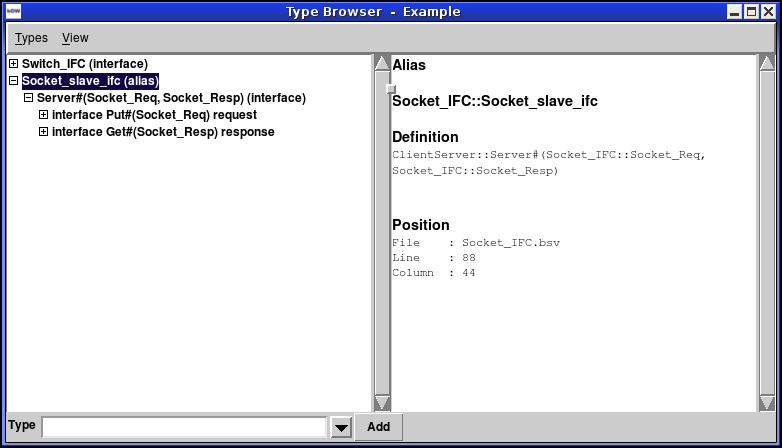
\includegraphics[width = 4 in]{figures/typebrowser}
\caption{Type Browser}
\label{fig-type}
\end{center}
\end{figure}


Before using the {\bf Type Browser} you must  {\bf Load} a
package  into the Development Workstation from the {\bf Package}
Window or the {\bf Type Browser}.  The following methods load a type into the Workstation:
\begin{itemize}
\item {\bf Send to Type} from the {\bf Package} Window
\item {\bf Type$\rightarrow$Add} from {\bf Type} pull down menu
\item {\bf Type} entry field at the bottom of the browser.
\end{itemize}

When using {\bf Type$\rightarrow$Add}, you can select a type or enter
a type (existing or new), in the entry window.  You can also add a new
type in the entry field at the bottom of the browser.  The arrow
provides a history function of all types you've entered in the field.

As in the {\bf Package} window, you can view the source code for any
type that you can modify, that is  the source (\te{.bsv}) file is
in the  search path of the project.
You cannot view (or edit) the source
code for any object defined in the BSC
libraries, since only compiled versions are
installed for these packages.

% -------------------------

\subsection{Using the Module Browser}

The {\bf Module Browser}, shown in Figure \ref{fig-modulebrowser},
provides a post-elaboration  view of
the instantiated module hierarchy.  It  also provides a
 link to an external \index{waveform viewer!using} waveform viewer, using
 the instantiated module hierarchy and  type definitions
along with waveform dump files to display additional Bluespec type data along
 with the waveforms.

The left side of the {\bf Module Browser} lists the loaded module
hierarchy.  The buttons along the right side of the window either open
the source code for a selected object  or send a selected signal to the
waveform viewer.

% -----

\subsubsection{Viewing the Module Hierarchy}

To view the   hierarchy of a module, you must first load the module into the
Workstation, either from the {\bf Module Browser} or {\bf Schedule
Analysis} window.  When a  module is loaded into the Workstation, both
the windows using the module will be updated.  The  windows are
 displaying different views of the same module.

You can expand the module hierarchy by clicking on the \te{+} icon or from
the {\bf View} menu.  The objects in the module hierarchy are
color-coded by type:
\begin{itemize}
\item Rules are in displayed in blue
\item Synthesized modules and primitives are in displayed in black
\item Most other object types, such as inlined modules,
\te{mkConnections}, and psuedo-hierarchies (such as \te{for-loops}), are displayed in gray.
\end{itemize}

You can view the source code of an object from  the {\bf View}
menu, the {\bf View Source} button,  or the context menu (right mouse
button) on the selected object.

% -----

\subsubsection{Viewing Waveforms with the Module Browser}

% add figures showing regular waveform and waveform from Workstation

\begin{figure}[ht]
\begin{center}
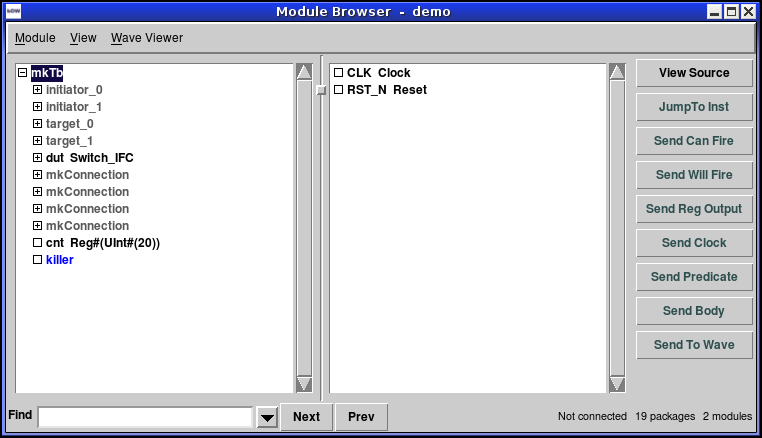
\includegraphics[width = 4.5 in]{figures/modulebrowser}
\caption{Module Browser}
\label{fig-modulebrowser}
\end{center}
\end{figure}

The Development Workstation  interfaces to separately
installed third-party  waveform viewers supplied by SpringSoft/Novas
and GtkWave,  appending type data and full type
hierarchies to the bit types typically displayed in  waveform
viewers.  When viewing designs through the Development Workstation
you can see signals with full type definition, including structures, structure
hierarchies, and  enumerated types, as shown in Figure~\ref{fig-waveviewer}.

\begin{figure}[ht]
\begin{center}
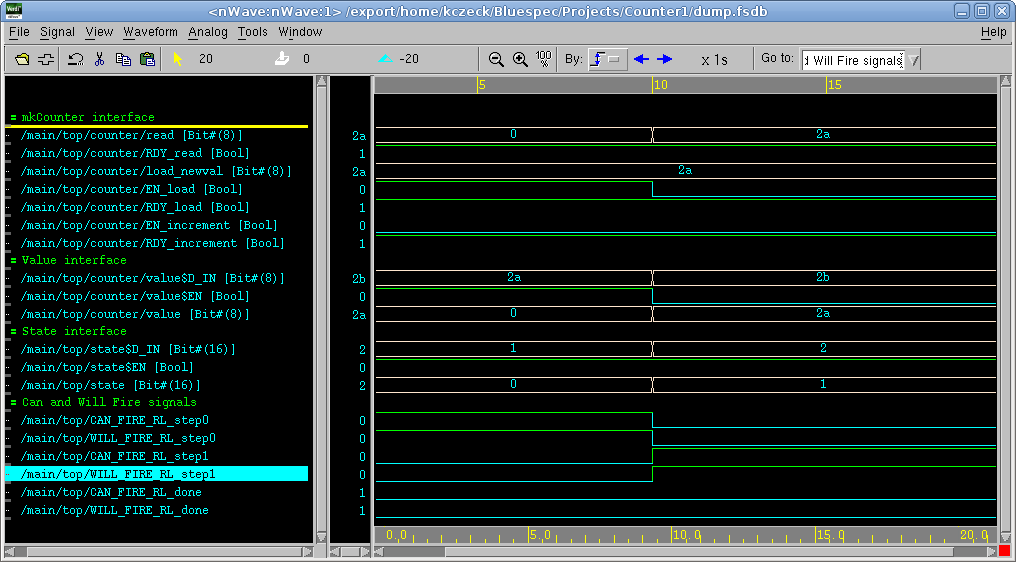
\includegraphics[width = 5 in]{figures/waveviewer}
\caption{Sample Waveforms}
\label{fig-waveviewer}
\end{center}
\end{figure}

\index{FSDB!Viewing}
\index{VCD!Viewing}
In order to view waveforms, you must have generated a waveform dump
file, either VCD or FSDB,  during simulation, as described in Section \ref{simulate}.   Only synthesized modules are
simulated and can be viewed with a waveform viewer.

Follow these steps to view waveforms from the Development Workstation:
\begin{enumerate}
\item Load the top module ({\bf Module$\rightarrow$Load Top Module})
to obtain  the module hierarchy from the \te{.bo} files.
\item Start or Attach the waveform viewer ({\bf Wave
Viewer$\rightarrow$Start} or {\bf Wave Viewer$\rightarrow$Attach}) to
initiate communication between the Workstation and the waveform
viewer. Note:  Many waveform viewers require an \te{xhost}
connection, which can be allowed through {\bf Wave
Viewer$\rightarrow$Allow XServer connections}.
\item Load the waveform dump file either from the Workstation ({\bf Wave
Viewer$\rightarrow$Load Dump File}) or from within the waveform viewer
itself.
\item Select an object and a \te{Send} action (for example {\bf Send
Can Fires}) to send the signal to the
viewer.
\end{enumerate}

%\paragraph{Viewing Waveforms for Rules}

Since state transitions in Bluespec are limited to within rule bodies,
viewing the various signals associated with rules can facilitate debug
and analysis of designs.  
The following signals  can be sent to the wave viewer:

\begin{itemize}
\item {\bf Send Can Fire} allows you to see the cycles in which the rule can be
scheduled to fire
\item {\bf Send Will Fire} allows you to see the cycles in which the
rule is scheduled to fire
\item {\bf Send Predicate} sends the values of the signals which
compose the explicit condition of the rule
\item {\bf Send Body} sends the values of the signals in the rule body
\end{itemize} 

These signals allow you to see when a rule is firing, and if
incorrect, the conditions which caused the rule to fire or not fire
as expected.

% -----

\subsubsection{Wave Viewer Commands}
You can record the commands used in your session and replay the
session to recreate the same waveforms as you modify your design by
checking the  {\bf WaveViewer$\rightarrow$Record Commands} option.  Once
selected,  you can  use the {\bf Save session}  and {\bf
Replay session} options.

% -----

\index{waveform viewer!options}
You can modify the waveform viewer settings directly from {\bf
WaveViewer$\rightarrow$Options}.  See Section \ref{options-waveform}
for more information about waveform viewer options.

If viewing FSDB files, the waves are compressed and you can view them
as they are created.  Select {\bf Waveform$\rightarrow$Auto Update}
from the waveform viewer and it will update the display every few
seconds.  This is especially useful when viewing long simulations.

% -------------------------

\subsection{Analyzing the Schedule}

The {\bf Schedule Analysis} window is for viewing and querying
information about the schedule for a single module. The following four
tabs   each display a different perspective of the schedule:
\begin{itemize}
\item Warnings: displays warnings generated by the compiler about scheduling decisions.
\item Rule Order: displays which methods are called by a selected rule.
\item Method Call: displays which rules use a selected method.
\item Rule Relations: displays conflicts between two selected rules.
\end{itemize}

 A module has to be loaded in the Workstation before you can view its scheduling
information.  If the
module has  not already  been loaded through another window, you can
load it from the {\bf Module$\rightarrow$Load} menu.  The Workstation
will read the BSC-generated files and load in the module and all
dependent modules.   You can load the entire project by loading the
top module ({\bf Module$\rightarrow$Load Top Module}).

The {\bf Schedule Analysis} window shows the schedule for a specific
module.  Since multiple modules may be loaded at the same time, use
the {\bf Module$\rightarrow$Set Module} option to chose the module for
analysis. The title bar of {\bf Schedule Analysis} window displays the
name of the active module.

% There are four tabs on the {\bf Schedule Analysis} window; each tab displays a different perspective of the schedule.  The {\bf
% Warnings} tab displays warnings about scheduling decisions made by the
% compiler. The {\bf
% Rule Order} tab shows which methods are called by a selected rule,
% while the {\bf Method Call} tab lists which rules  use a selected
% method.  The {\bf Rule Relations} tab displays conflicts between any
% two selected rules.

% -----

\subsubsection{Warnings}
\index{compiler messages}

\begin{figure}[ht]
\begin{center}
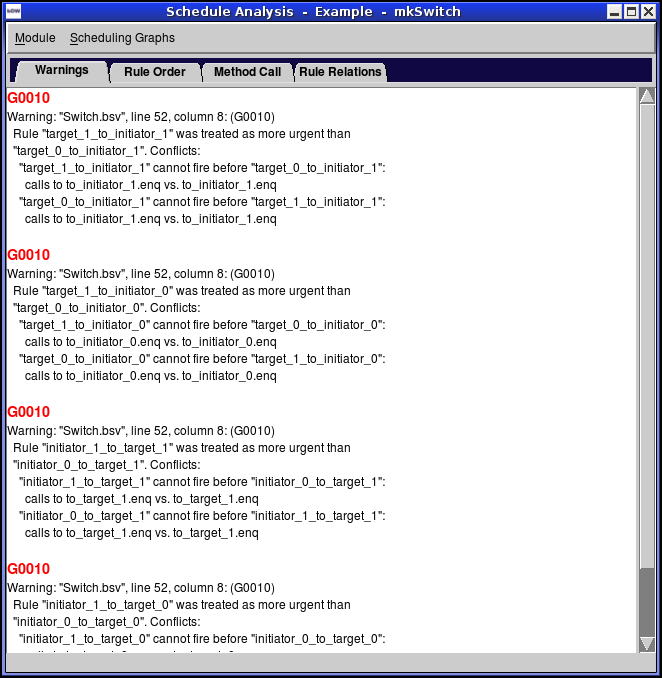
\includegraphics[width = 3.5 in]{figures/schedule_warnings}
\caption{Schedule Browser - Warnings Tab}
\label{fig-warn}
\end{center}
\end{figure}

% The compiler generates warnings when it is required to make scheduling
% decisions about either the static execution of rules or the rule
% urgency.

The  {\bf Warnings} tab displays two types of warnings: static
execution warnings and urgency warnings,  as shown in Figure \ref{fig-warn}.
These are the same warnings displayed during compilation.

When  three or more rules cannot  execute in
the same cycle, even though any two of the rules can, the compiler
will introduce a conflict between two of the rules and generate a
static execution warning message.

When two rules conflict and the user has not specified the urgency of
the rules, the compiler generates an urgency warning, indicating that
it has made  an
arbitrary choice as to which rule is more urgent.

Refer to the BSC documentation for more description of scheduling
messages in more detail.

% -----

\subsubsection{Rule Order}
\begin{figure}[ht]
\begin{center}
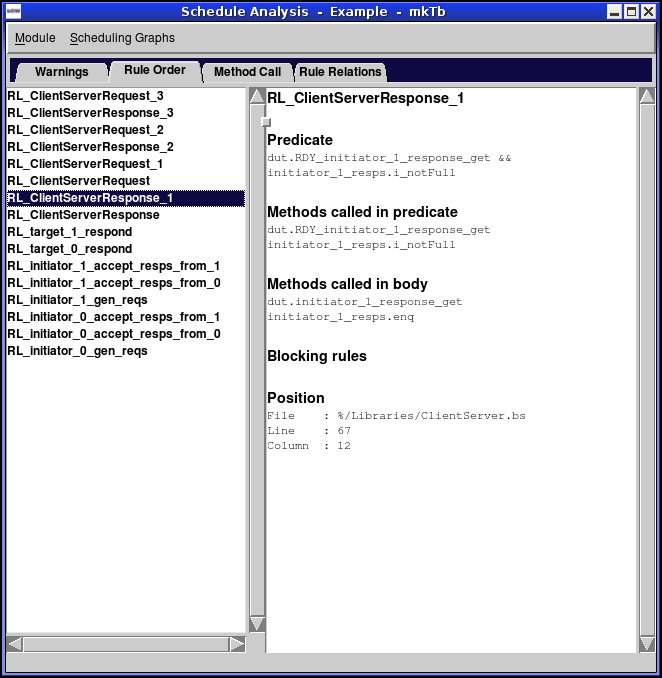
\includegraphics[width = 3.5 in]{figures/schedule_ruleorder}
\caption{Schedule Browser - Rule Order Tab}
\label{fig-ruleorder}
\end{center}
\end{figure}

The {\bf Rule Order} tab, shown in Figure \ref{fig-ruleorder},
displays the rules in execution order, one per line.
The window is divided in two panes; the left listing the
rules and methods in the module in execution order, the right
displaying information about the selected rule or method.  When you
select a rule from the left pane, the right pane displays the
following details:


\begin{itemize}

\item Predicate or condition to fire

\item Methods called

\item Blocking rules - scheduling conflicts which block execution
\item Position in the source file


\end{itemize}

The predicate is the condition for the rule to fire.  If the predicate is \te{True}, the rule fires every cycle.  If it is
\te{False}, it never fires.

To view the source for a rule, select {\bf Module$\rightarrow$View Source}.  It
will open an editor window with the source file in which the rule is
defined,  at the position indicated on the right pane.  If no
position is listed, the rule or method is part of the BSC library and
cannot be modified and the source file cannot be opened.

% -----

\subsubsection{Method Call}

\begin{figure}[ht]
\begin{center}
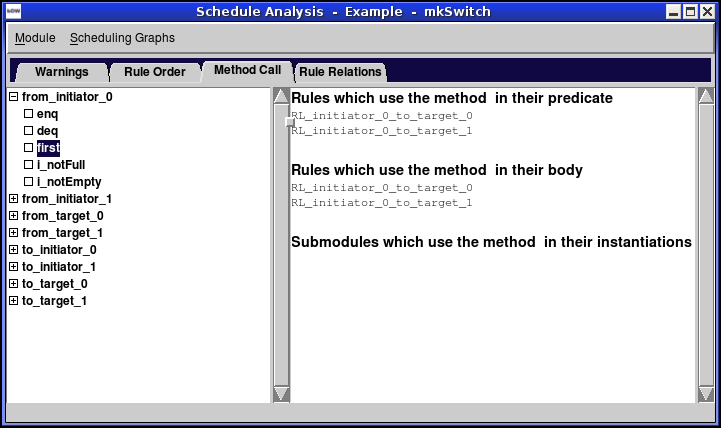
\includegraphics[width = 3.5 in]{figures/schedule-methodcall}
\caption{Schedule Browser - Method Call Tab}
\label{fig-methodcall}
\end{center}
\end{figure}

The {\bf Method Call} tab displays all instances of method calls in
the module.  It is divided into two panes,
as shown in Figure \ref{fig-methodcall}.  The left pane lists the
method calls by module instance.  The right pane displays information
on the object selected in the left pane.

When first opened, the left pane displays a list of module instances.
To display the method calls for each instance, click on the expand
icon next to the method.

When an instance is selected, the right pane
displays more detail about the module instance: the module,  the input and output ports and, if
available, the position  in the source code.
To view the source for an instance, select {\bf Module$\rightarrow$View Source}.  It
will open an editor window with the source file in which the instance is
defined,  at the position indicated on the right pane.  If no
position is listed, the module is part of the BSC library and
cannot be modified, and therefore,  the source file cannot be opened.

When a method is selected, the rules and submodules which use the
method are displayed in the right pane.

% -----

\subsubsection{Rule Relations}
\begin{figure}[ht]
\begin{center}
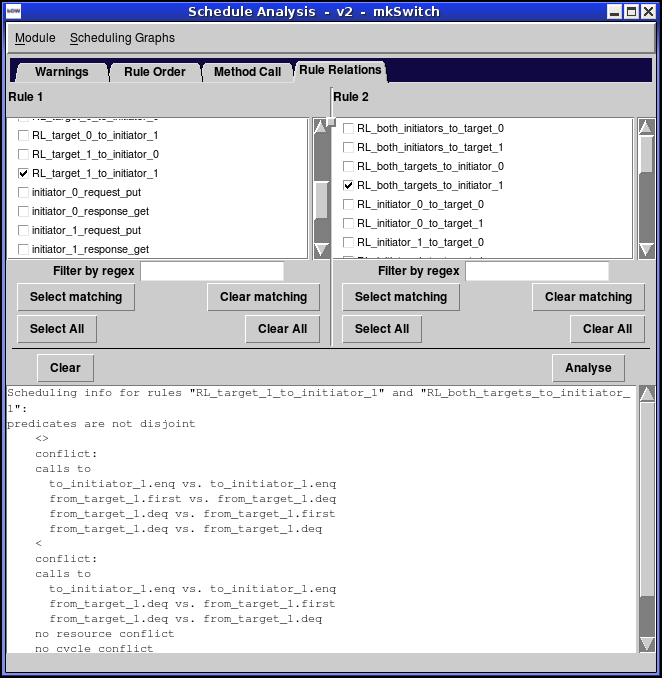
\includegraphics[width = 3.5 in]{figures/schedule_rulerel}
\caption{Schedule Browser - Rule Relations Tab}
\label{fig-rulerel}
\end{center}
\end{figure}

The {\bf Rule Relations} tab  displays a listing with scheduling
information for each pair of rules
% .describes conflicts between
% any two rules,
as shown in Figure \ref{fig-rulerel}. This
is the same information generated from the  \te{-show-rule-rel}
compile flag.

If the compiler can determine that the predicates
of the two rules are mutually exclusive (disjoint), then the two rules
can never be ready in the same cycle and therefore conflicts are
irrelevant and will not be computed.

For each conflict found, the conflicting calls are listed.
The  types of conflicts are as follows:
\begin{itemize}
\item$<>$: The rules use a pair of methods which are not
conflict free.  The rules either cannot be
executed in the same clock cycle or they can but one must be sequenced
first.  The compiler lists the methods used in each rule which are the
source of the conflict.
\item$<$: The first rule cannot be executed in sequence
before the second rule, because they
use methods which cannot sequence in that order.  Again, the compiler
lists  the methods used in each rule
which are the source of the conflict.
\item resource: A conflict introduced because of resource
arbitration, where more rules are vying for a method than there are
available ports for the method.
\item cycle: A conflict introduced by the compiler to break an
execution order cycle.

\index{attributes!preempts}
\index{preempts@\te{preempts} attribute}
\item attribute: A conflict introduced by a scheduling
attribute, such as the \te{preempts} attribute.
\end{itemize}

% -------------------------

\subsection{Viewing Scheduling Graphs}
\index{scheduling graphs}
\index{-sched-dot@\te{-sched-dot} (compiler flag)}
  The {\bf Scheduling Graphs}
option on the {\bf Schedule Analysis}  displays the scheduling graphs.
To view  the graphs, the following conditions must be met:
\begin{itemize}
\index{graphviz}\index{Tcldot}
\item The graphviz Tcl extensions (Tcldot)  must be installed as
described in Section~\ref{graphviz-install}.
\item  The \te{.dot} files must have been generated during
compilation by specifying the  compiler flag \te{-sched-dot} in the options
field on  the {\bf Project Options$\rightarrow$Compiler} tab.
\item You must have a synthesized module.
% \item A module must be loaded in the Workstation.  You can load a module into the Workstation from {\bf
% Module$\rightarrow$Load} or you could  have previously
% loaded a module  in the {\bf Module Browser}.
\end{itemize}

The following five graphs are available for each synthesized module:
\begin{itemize}
\item Conflict
\item Execution Order
\item Urgency
\item Combined
\item Combined Full
\end{itemize}

In each of these graphs, the nodes are rules and methods and the edges
represent some relationship between pairs of rules/methods.  Methods are represented by a box and rules are represented by
an ellipse, so that they are visually distinguishable.

\index{filter}

 You can perform the following tasks for each of the {\bf Scheduling Graphs}:
\begin{itemize}
\item Filter the graph  by selecting
specific nodes and edges to display or to remove from the graph.  The  conflict
graph in Figure \ref{fig-conflictgraph} shows the filter options on
the left side of the window.

\item Change the text label on the graph with the {\bf Rename} button.

\item Hide the filter options with the  {\bf Hide} button.  Use {\bf
View$\rightarrow$Show Filter} to unhide the filter options.

\item Save the graph as a file from the  {\bf View$\rightarrow$Export}
menu.  You will be prompted for a name  and format for the export file.

\item  Zoom by using the {\bf Zoom} menu or the slide bar at
the top of the screen.
\end{itemize}

% -----

\subsubsection{Conflict}

\index{scheduling graphs!conflict}
\index{conflict (scheduling graph)}

\begin{figure}[ht]
\begin{center}
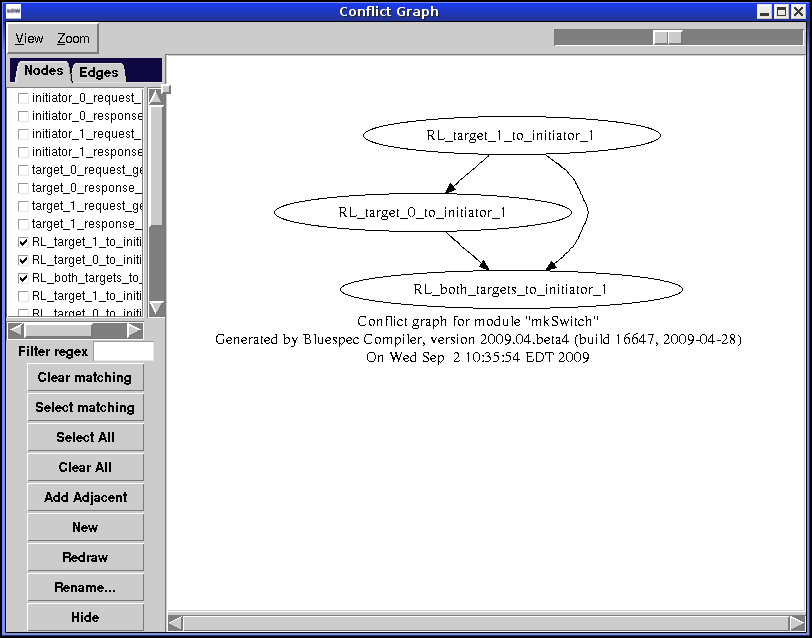
\includegraphics[width = 3 in]{figures/conflictgraph}
\caption{Conflicts Graph with filter options}
\label{fig-conflictgraph}
\end{center}
\end{figure}

The conflicts graph, shown in Figure \ref{fig-conflictgraph},  displays rules/methods which conflict either completely
(they cannot execute in the same cycle) or  in one direction (if they execute in the
same cycle, it has the be in the opposite order).  Complete conflicts are
represented by bold non-directional edges. Ordering conflicts are
represented by dashed directional edges, pointing from the node which must
execute first to the node which must execute second.

% \begin{figure}[ht]
% \begin{center}
% 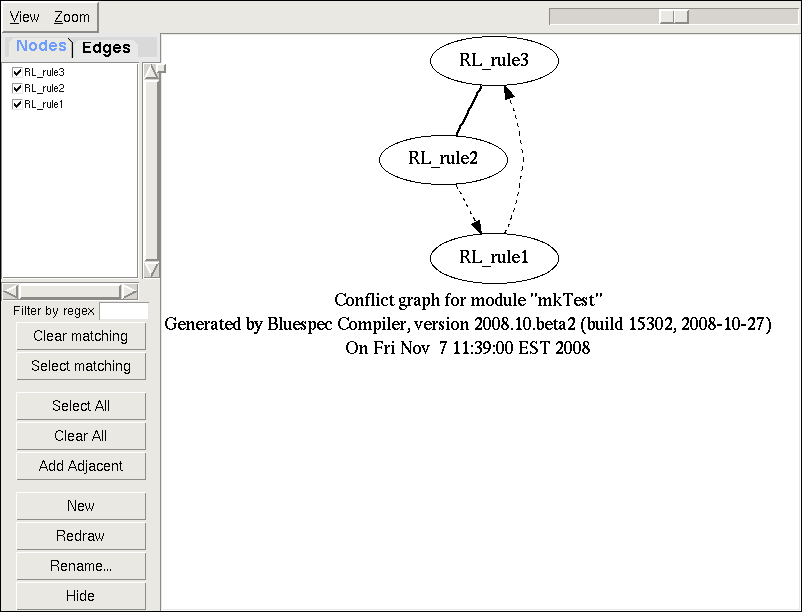
\includegraphics[height = 1.8 in]{figures/conflictcycle}
% \caption{Conflicts Graph Displaying Execution Cycle}
% \label{fig-conflictcycle}
% \end{center}
% \end{figure}

When a group of nodes form an execution cycle, as shown in Figure \ref{fig-conflictgraph}, the compiler breaks the cycle by turning one of the edges into
a complete conflict and emits a warning.  This graph is generated before
that happens, so it includes any cycles and can be used to debug any such
warnings.

% -----

\subsubsection{Execution Order}
\index{scheduling graphs!execution order}
\index{execution order (scheduling graph)}


% \begin{figure}
% \begin{minipage}[ht]{3 in}
% \begin{center}
% 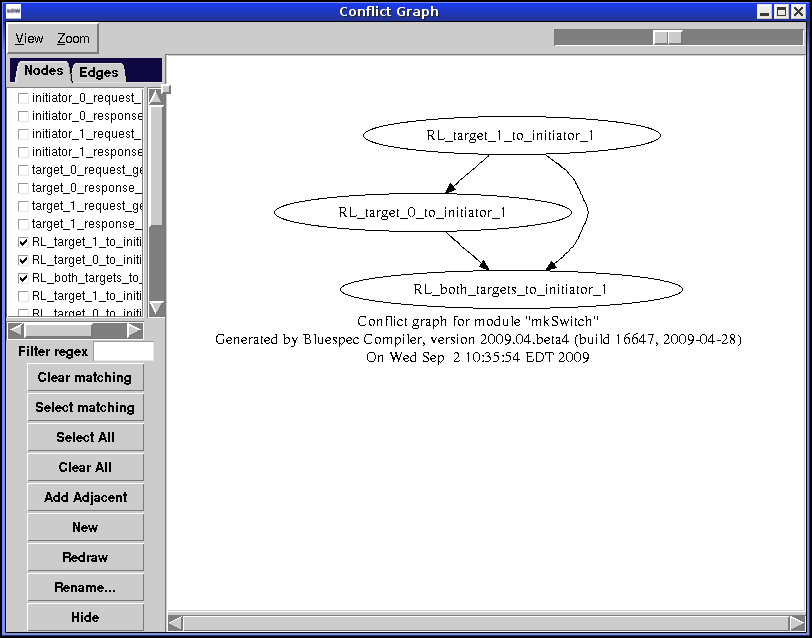
\includegraphics[width = 3 in]{figures/conflictgraph}
% \caption{Conflicts Graph with filter options}
% \label{fig-conflictgraph}
% \end{center}
% \end{minipage}
% \hspace{.3 in}
% \begin{minipage}[ht]{3 in}
% \begin{center}
% 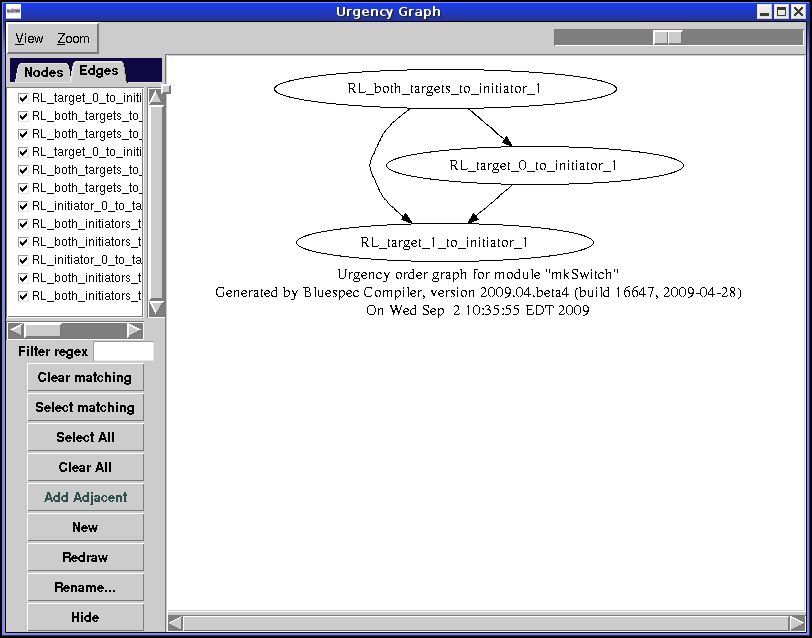
\includegraphics[width = 3 in]{figures/urgencygraph}
% \caption{Urgency Graph with filter options }
% \label{fig-executiongraph}
% \end{center}
% \end{minipage}
% \end{figure}



\begin{figure}[htbp]
\begin{center}
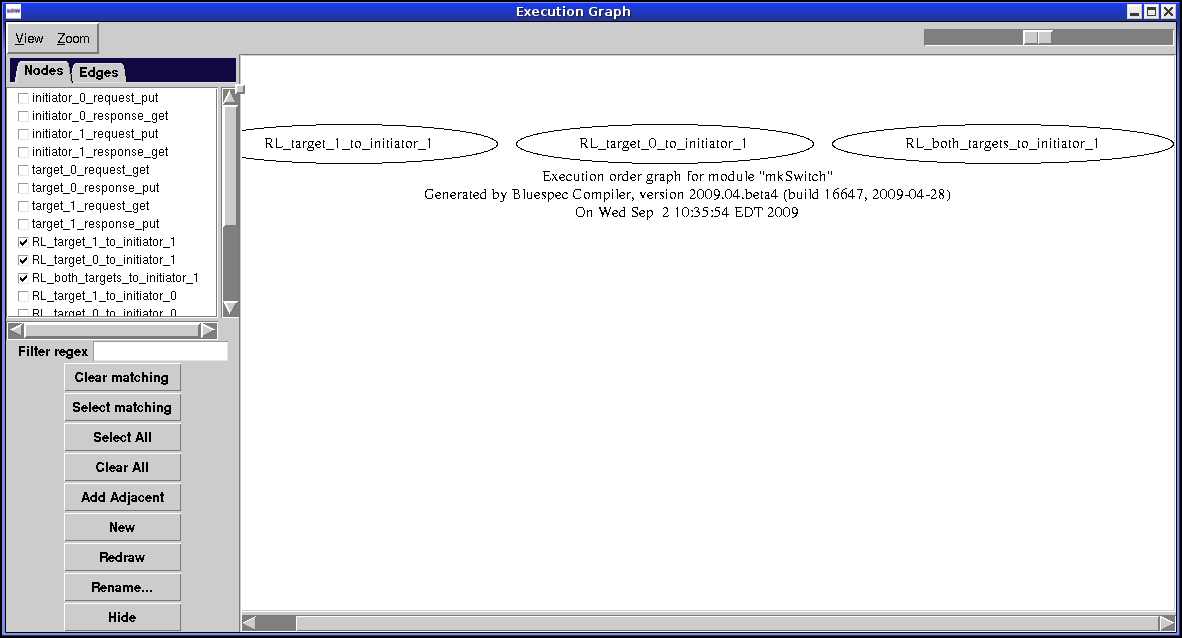
\includegraphics[width = 4.5 in]{figures/executiongraph}
\caption{Execution Order Graph with filter options }
\label{fig-executiongraph}
\end{center}
\end{figure}


The execution order graph, shown in Figure \ref{fig-executiongraph},  is similar to the conflicts graph, except that it only includes
the execution
order edges; the full-conflict edges have been dropped.  As a result,
there is no need to distinguish between the types of edges (bold versus
dashed), so all edges appear as normal directional edges.

This graph is generated after cycles have been broken and therefore
describes the final execution order for all rules/methods in the
module.

% -----

\subsubsection{Urgency}
\index{attributes!descending\_urgency}
\index{descending\_urgency@\te{descending\_urgency} attribute}
\index{scheduling graphs!urgency}
\index{urgency (scheduling graph)}

\begin{figure}[htbp]
\begin{center}
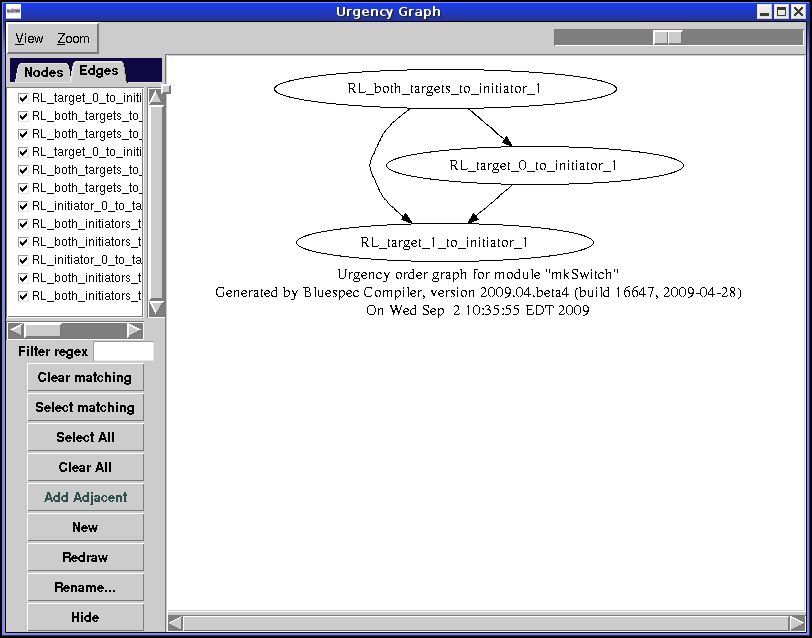
\includegraphics[width = 3 in]{figures/urgencygraph}
\caption{Urgency Graph with filter options}
\label{fig-urgencygraph}
\end{center}
\end{figure}

The edges in the urgency  graph, as shown in Figure \ref{fig-urgencygraph}, represent urgency dependencies.  They are
directional edges which point from a more urgent node to a less urgent
node (meaning that if the rules/methods conflict, then the more urgent
one will execute and block the less urgent one).  Two rules/methods
have an edge either because the user specified a \te{descending\_urgency}
attribute or because there is a data path (though method calls) from
the execution of the first rule/method to the predicate of the second
rule/method.

If there is a cycle in the urgency graph, the compiler  reports an error.
This graph is generated before such errors, so it will contain any
cycles and is available to help debug the situation.

% -----

\subsubsection{Combined}
\index{scheduling graphs!combined}
\index{combined (scheduling graph)}


\begin{figure}
\begin{minipage}[ht]{3 in}
\begin{center}
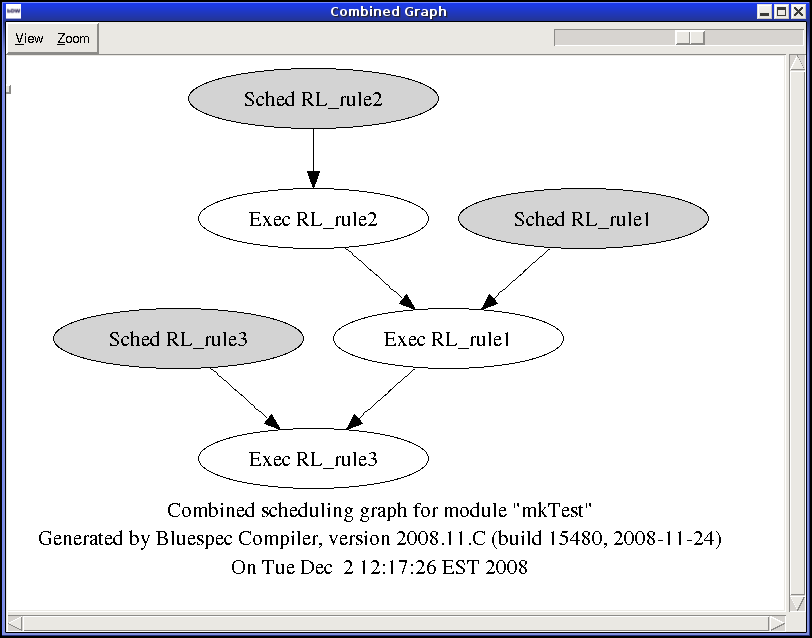
\includegraphics[width = 3 in]{figures/combinedgraph}
\caption{Combined Graph}
\label{fig-combinedgraph}
\end{center}
\end{minipage}
\hspace{.3 in}
\begin{minipage}[ht]{3 in}
\begin{center}
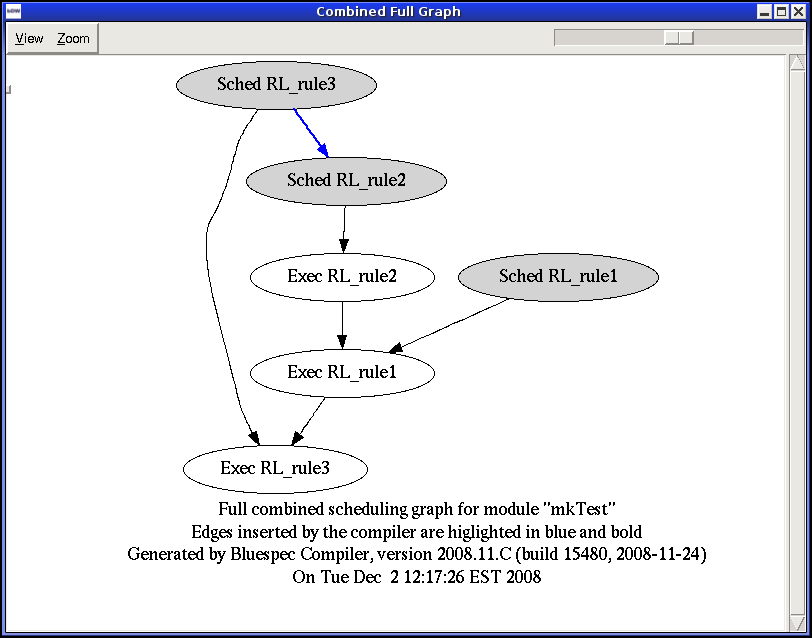
\includegraphics[width = 3 in]{figures/combinedfullgraph}
\caption{Combined Full Graph}
\label{fig-combinedfullgraph}
\end{center}
\end{minipage}
\end{figure}



% \begin{figure}[htbp]
% \begin{center}
% 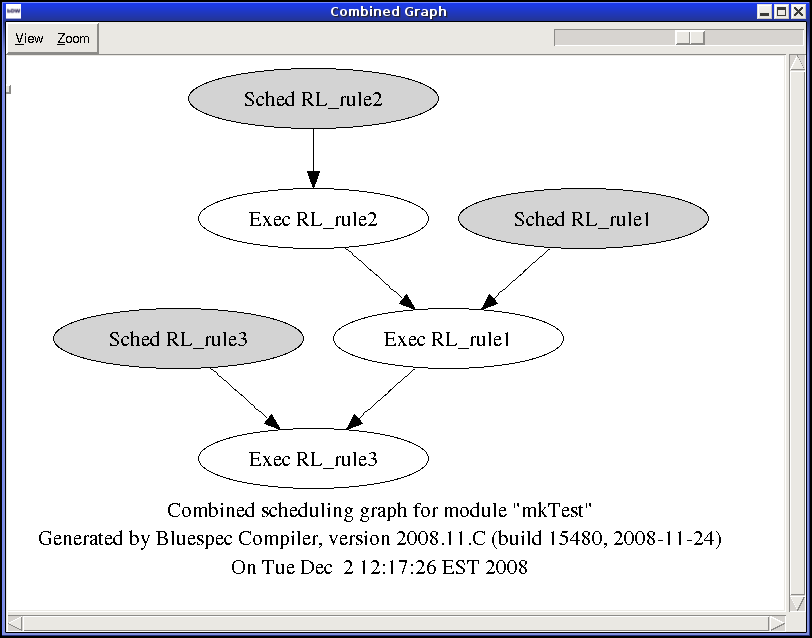
\includegraphics[width = 3.5 in]{figures/combinedgraph}
% \caption{Combined Graph }
% \label{fig-combinedgraph}
% \end{center}
% \end{figure}

% \begin{figure}[htbp]
% \begin{center}
% 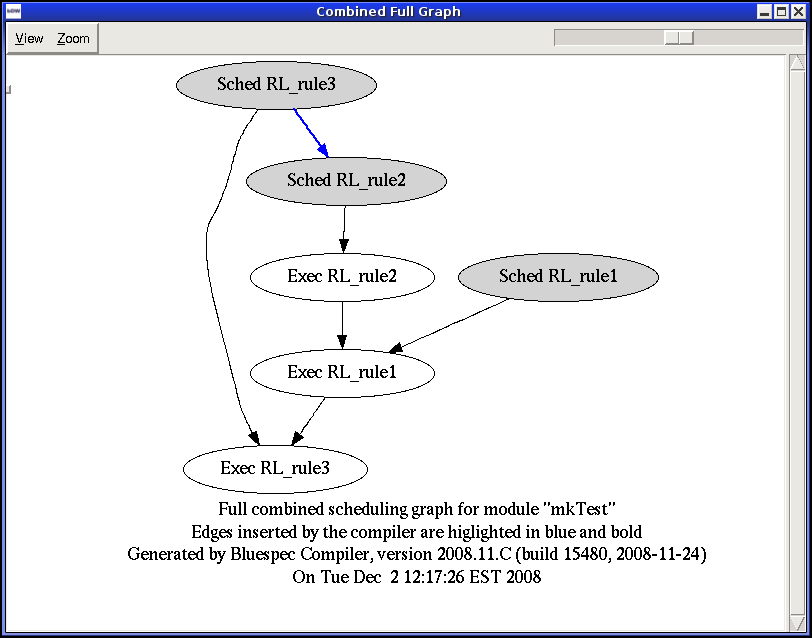
\includegraphics[width = 3.5 in]{figures/combinedfullgraph}
% \caption{Combined Full Graph }
% \label{fig-combinedfullgraph}
% \end{center}
% \end{figure}


In the combined graph, shown in Figure \ref{fig-combinedgraph} and the
combined full graph, shown in Figure \ref{fig-combinedfullgraph},
 there are two nodes for each rule/method.
One node represents the scheduling of the rule/method (computing the
\te{CAN\_FIRE} and the \te{WILL\_FIRE} signals)
and one node represents the execution of the rule/method's body.  The
nodes are labelled \te{Sched} and \te{Exec} along with the
rule/method name. To further help visually distinguish the nodes, the
\te{Sched} nodes are shaded.

The edges in this graph are a combination of the execution order
and urgency graphs.  This is the graph in which the
microsteps of a cycle are performed: compute whether a rule will fire,
execute a rule, and so on.

In the rare event that the graph has a cycle, the compiler will report an error.
This graph is generated prior to that error, so it will contain the
cycle and be available to help in debugging the situation.

% -----

\subsubsection{Combined Full}
\index{scheduling graphs!combined full}
\index{combined full (scheduling graph)}

Sometimes the execution or urgency order between two rules/methods is
underspecified and either order is a legal schedule.  In those cases,
the compiler
picks an order and warns the user that it did so.

The combined full  graph, shown in Figure \ref{fig-combinedfullgraph} is the same as the combined graph above, except that it includes the
arbitrary edges which the compiler inserted.  The new edges are bold
and colored blue, to help highlight them visually.

This is the final graph which determines the static schedule of a module
(the microsteps of computing predicates and executing bodies).

As with the above graph, there are separate \te{Sched} and \te{Exec} nodes
for each rule/method, where the \te{Sched} nodes are shaded.

% ------------------------------------------------------------
% Section: Workstation Tools

\section{Workstation Tools}

Additional features provided by the Development Workstation are found
on the \te{Tools} menu on the main menu bar.

% -------------------------

\subsection{Backup}
\index{backup}
Use the {\bf Backup Project} option on the {\bf Project} menu, shown
in Figure \ref{fig-backup},   to create
a tar file of your project.  You
 choose which files to include by file type.  The default is to
include all the \te{.bsv} files from the search path.

\begin{figure}[ht]
\begin{center}
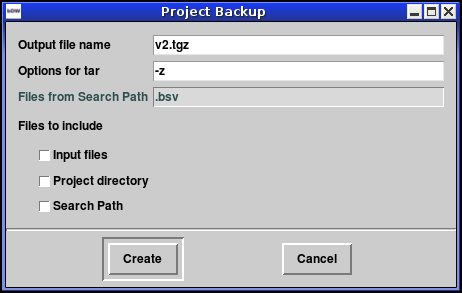
\includegraphics[height = 2 in]{figures/backup}
\caption{Backup Project Window}
\label{fig-backup}
\end{center}
\end{figure}

% -------------------------

\subsection{Export Makefile}
\index{makefile!exporting}

Use the {\bf Export Makefile} option on the {\bf Project} menu to
generate a Makefile based on the parameters set in the {\bf Project
Options}.  The Makefile will include the following
targets:
\begin{itemize}
\item compile
\item link
\item simulate
\item clean
\item full\_clean
\end{itemize}

The Development Workstation will prompt you for the directory and name
of the Makefile.  The default is to create a file named \te{Makefile}
in the project directory.

% -------------------------

\subsection{Import BVI Wizard}
\index{import BVI}
\index{wizard (import BVI)}
\index{import BVI wizard}

The \te{import "BVI"} statement creates a BSV wrapper for an RTL
module,  defining the  port connections and associating them with BSV
interfaces and methods.  This mechanism allows you to
include existing RTL files in BSV designs.
  The  \te{import BVI} wizard   helps  you
 create the BSV wrapper including  the
\te{import "BVI"} statement.  The \te{import "BVI"} statement is
described in more detail in the BSV Reference Guide, in the section
{\em Embedding RTL in BSV design}.

In the first step of the wizard you enter the RTL statements, either
by reading   the RTL file,  reading a
specification file, or by manually entering the parameters,  input, and
output statements.
While the wrapped file can be any type of  RTL file,  the
 Workstation can only read in Verilog files.  For other types of RTL
 files (such as VHDL), you can read a specification file or manually
 enter the ports.  You then proceed through the steps of the wizard to
 complete the BVI import statement. Throughout this section we'll refer to
Verilog files, but you could also use the same procedure to wrap any RTL file.


The wizard has six steps:
\begin{enumerate}
\item Verilog Module Overview: Review the Verilog parameters, inputs,
outputs, and inouts
\item Bluespec Module Definition: Define the module header for the
\te{import "BVI"} statement
\item Method Port Binding: Define the \te{method} statements
\item Combinational Paths: Define the \te{path} statements
\item Scheduling Annotations: Define the \te{schedule} statements
\item Finish: Review, compile, and save the Verilog wrapper.
\end{enumerate}

Each step has a \te{Check} button, which verifies the information
entered on the screen, and a \te{Show} button which displays the BSV
code for the information entered so far (it does not look ahead to
information entered in later steps).  When  viewing the statement
displayed via the \te{Show} screen, you
can verify that the code will compile with the \te{Compile} button.
Compiler messages are displayed in the main Workstation window, as always.

Throughout the wizard,  Verilog statements are displayed in gray and the
corresponding Bluespec statements are displayed in blue.

% -----

\subsubsection{Step 1: Verilog Module Overview}
\index{.info file}

The first step, shown in Figure \ref{fig-importbvi1},  defines the
Verilog module, including the module
name, parameters, inputs, outputs, and inouts.  There are three ways
to define the module:
\begin{itemize}
\item Read in an existing Verilog file
\item Read in a specification  file  (\te{.info})
\item Enter the information manually
\end{itemize}

\begin{figure}[htbp]
\begin{center}
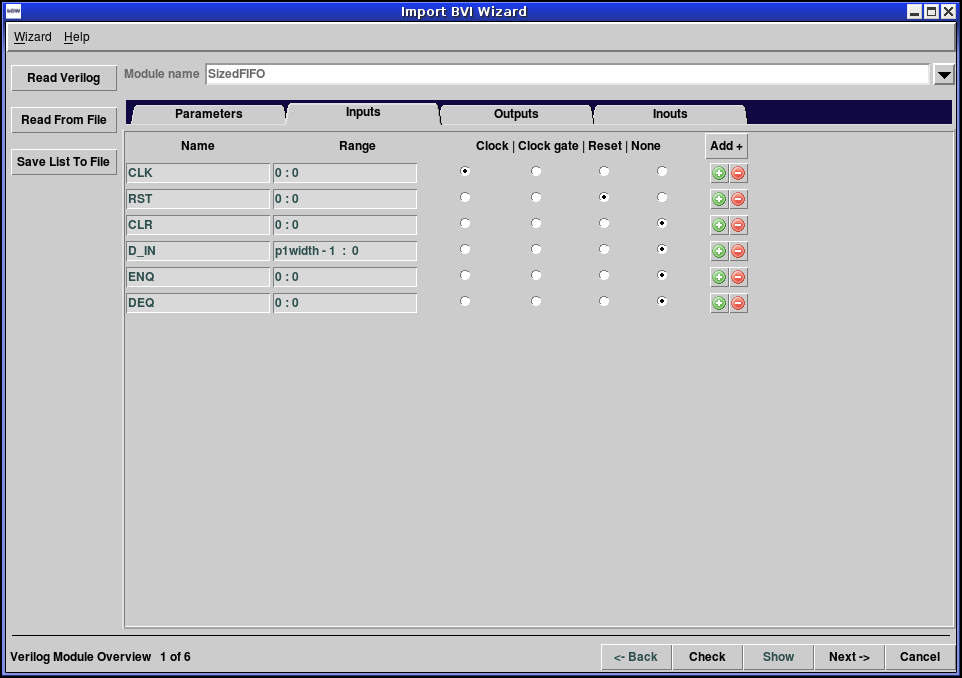
\includegraphics[width = 4.5 in]{figures/importbvi1}
\caption{Step 1: Verilog Module Overview }
\label{fig-importbvi1}
\end{center}
\end{figure}

Once the information has been entered, you can modify any of the
fields directly in the wizard.  There is a tab for each statement
type: \te{Parameters}, \te{Inputs}, \te{Outputs}, and \te{Inouts}.
You can generate a \te{.info} file describing the Verilog inputs and
outputs, with the \te{Save List to File} button.


\paragraph{Specification file}

The specification (\te{.info}) file is useful when you don't have a
 Verilog file, but do have RTL specifications.  The file is used
 to prefill the wizard with whatever
 information  is available. Each line in the \te{.info}
 file contains a single element: module,
parameter, input, output, or inout, along with the element name.  If known,
the Verilog range or type, and attributes can also be specified. Each line ends
with a semicolon.   The file does not have to contain the complete
 specification.  You can generate a \te{.info} file in any text
 editor.  You can also export the information within the wizard to
 a specification file with the \te{Save List to File} button.




\begin{tabular}{|l|l|}
\hline
\multicolumn{2}{|c|}{.info file layout} \\
\hline
&valid values for attribute\\
\hline
{\bf module} \emph{modulename} {\bf ;}&\\
{\bf parameter} \emph{parametername} range/type{\bf ;}&\\
{\bf input} \emph{inputname} range attribute{\bf ;}&\te{clock, clock\_gate, reset, none}\\
{\bf output} \emph{outputname} range attribute{\bf ;}&\te{clock, clock\_gate,
reset, registered, none}\\
\hline
\end{tabular}


Example - SizedFIFO .info file:

\begin{verbatim}
module SizedFIFO;
parameter p1width 1;
parameter p2depth 3;
parameter p3cntr_width 1;
parameter guarded 1;
input CLK {0 : 0} clock;
input RST {0 : 0} reset;
input CLR {0 : 0} none;
input D_IN {p1width - 1  :  0} none;
input ENQ {0 : 0} none;
input DEQ {0 : 0} none;
output FULL_N {0 : 0} none;
output EMPTY_N {0 : 0} none;
output D_OUT {p1width - 1  :  0} none;
\end{verbatim}

% -----

\subsubsection{Step 2: Bluespec Module Definition}

In the second step of the wizard you define the module  header and map
the Verilog inputs  to BSV values.  The module
header includes the interface type provided by the module and Bluespec
module arguments.  You can use an
existing interface, in which you'll also select the package where the
interface is defined, or define a new interface from the methods.
The fields on the left side of the screen of step 2,  as shown in
Figure \ref{fig-importbvi2},  define the module
header, while the fields on the right side of the screen define the
BSV to Verilog bindings.


\begin{figure}[htbp]
\begin{center}
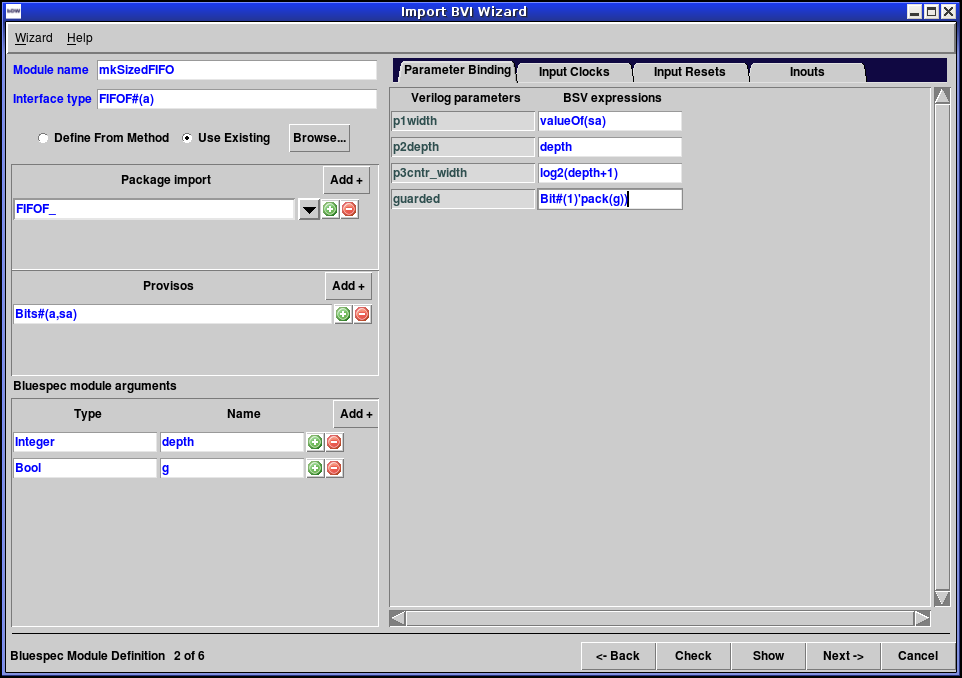
\includegraphics[width = 5 in]{figures/importbvi2}
\caption{Step 2: Bluespec Module Definition }
\label{fig-importbvi2}
\end{center}
\end{figure}


The module name defaults to the name of the Verilog module, prefaced
with \te{mk}.  Continuing the previous example, the Bluespec module
\te{mkSizedFIFO} is created for the Verilog module \te{SizedFIFO}.
The module returns an interface, either an  existing
interface or  a new interface based on the methods.

To use an existing interface, select the {\bf Use Existing}
button.  You can type in the name of an existing interface or
 use the {\bf Browse} button
to display all available packages, including library packages, and
the interfaces defined in each package.   In this example we'll  use the
\te{FIFOF\#(a)} interface from the
\te{FIFOF} package.  When using an existing interface, you must
import the package which defines the interface.  In this example, the
generated Bluespec wrapper will include the \te{import} statement for
the \te{FIFOF} package.

 Select {\bf Define from
Method} to define a new interface.  You'll need to provide a name for
the new interface
type. The rest of  the interface will be defined in  step 3 of the
wizard.  Instead of including an \te{import} statement, an interface
declaration will be added to the wrapper   (\te{.bsv}) file generated.


All arguments and return values in the BSV wrapper must be in the \te{Bits}
class or be of type \te{Clock}, \te{Reset}, \te{Inout} or a
subinterface which meets these requirements.  The {\bf Provisos} for
the \te{FIFOF} example indicate that the data type of the FIFO,
(\te{a}), along with the size of \te{a}, (\te{sa}), must both be in the
\te{Bits} class.  Finally, the module arguments are defined (\te{depth}
and \te{g} in our example).  The information entered is   enough to define
the module header  as follows:

\begin{verbatim}
import "BVI" SizedFIFO =
module mkSizedFIFO #(Integer depth, Bool g) (FIFOF#(a))
        provisos(Bits#(a,sa));
\end{verbatim}


The first tab ({\bf Parameters}) on the right hand side of the screen
connects the Verilog ports to the BSV parameters. Note that the BSV
module's parameters have no inherent relationship to the Verilog
module's parameters.  These fields  define the BSV expressions for
the Verilog parameters, completing the \te{parameter} statements. The
parameter statements for our example are:

\begin{verbatim}
        parameter p1width = valueOf(sa);
        parameter p2depth = depth;
        parameter p3cntr_width = log2(depth+1);
        parameter guarded = Bit#(1)'(pack(g));
\end{verbatim}

The {\bf Input Clocks} and {\bf Input Resets} tabs define how the BSV
clocks correspond to the Verilog clocks.  The BSV clock defaults to
\te{clk\_}{\em Verilogclockname}.  The BSV reset defaults to
\te{rst\_}{\em Verilogresetname}.    Our example generates the
following clock statements:
\begin{verbatim}
        default_clock clk_CLK (CLK);
        default_reset rst_RST_N (RST) clocked_by (clk_CLK);
\end{verbatim}

You can view the complete wrapper generated at this
point in the wizard   using the \te{Show} button.  Notice how the
\te{import FIFOF:: *:} statement is included, since that is the
package defining the \te{FIFOF} interface.
\begin{verbatim}
import FIFOF::*;

import "BVI" SizedFIFO =
module mkSizedFIFO #(Integer depth, Bool g) (FIFOF#(a))
        provisos(Bits#(a,sa));

        parameter p1width = valueOf(sa);
        parameter p2depth = depth;
        parameter p3cntr_width = log2(depth+1);
        parameter guarded =  Bit#(1)'(pack(g));

        default_clock clk_CLK (CLK);
        default_reset rst_RST_N (RST) clocked_by (clk_CLK);
endmodule
\end{verbatim}

If you {\bf Compile} the wrapper as defined at this point, you will
see compiler errors, since the statement is not complete.

% -----

\subsubsection{Step 3: Method Port Binding}

Step 3 of the  wizard builds the method statements  connecting
the methods in the Bluespec interface to the associated Verilog wires.
How the default method statements are built depends on the type of
interface you are using:
\begin{itemize}
\item If you are using an existing interface,  the method
statements will be based on the methods in the interface declaration.
Check  {\bf Use Existing} and then   select {\bf Build Skeleton} to
start declaring the method statements.
\item If the interface type is {\bf Define from Method}, the methods will be
based on the Verilog statements.  Use
{\bf Auto Create from Verilog} to build the method statements.
\end{itemize}

 Ports, methods, and subinterfaces  are listed in the left
box, as shown in Figure \ref{fig-importbvi3}.  To view the  bindings, or connections between the BSV object
and the Verilog wires,  check the box next to the BSV object to
display the bindings for that object.


\begin{figure}[htbp]
\begin{center}
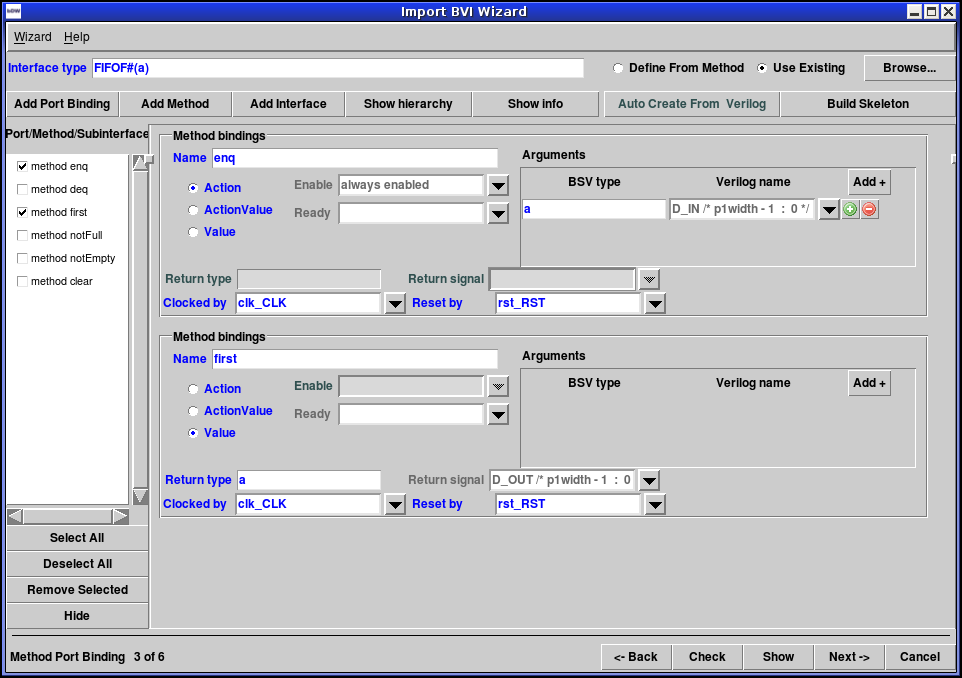
\includegraphics[width = 5 in]{figures/importbvi3}
\caption{Step 3: Method Port Binding }
\label{fig-importbvi3}
\end{center}
\end{figure}


The port bindings correspond to the \te{port} statements within the
\te{import "BVI"} statement.  The \te{port} statement declares an input
port which is not part of a method, along with the value to be passed
to the port.  While parameters must be compile-time constants, ports
can be dynamic.

There will only be interfaces when there are subinterfaces  in the BSV
interface declaration.


\paragraph{Build Skeleton}
 This option defines the method bindings when you are using an
 existing interface.  It creates an \te{import "BVI" method}
statement for each method in the  interface declaration.  The method
type (\te{Action, value, ActionValue}) is taken directly from the
interface method declaration.  Fill in the missing
Verilog  bindings to complete the method statements as follows:
\begin{itemize}
\item The Verilog names for BSV arguments
\item Verilog bindings for the  \te{Enable} and
\te{Ready} signals (the  \te{Ready} signals can often
be left blank).
\item \te{Return} signals for \te{value} methods
\end{itemize}


% Example using {\bf Build Skeleton} and the existing \te{FIFOF}
% interface for the \te{mkSizedFIFO} example:

% \begin{verbatim}
% import FIFOF::*;

% import "BVI" SizedFIFO =
% module mkSizedFIFO #(Integer depth, Bool g) (FIFOF#(a))
% 	provisos(Bits#(a,sa));

% 	parameter p1width = valueOf(sa);
% 	parameter p2depth = depth;
% 	parameter p3cntr_width = log2(depth+1);
% 	parameter guarded = g;

% 	default_clock clk_CLK;
% 	default_reset rst_RST_N;

% 	input_clock clk_CLK (CLK)  <- exposeCurrentClock;
% 	input_reset rst_RST_N (RST_N) clocked_by(clk_CLK)  <- exposeCurrentReset;


% 	method enq (D_IN /*p1width-1:0*/)
% 		 enable((*inhigh*)enq_enable) clocked_by(clk_CLK) reset_by(rst_RST_N);
% 	method deq ()
% 		 enable((*inhigh*)deq_enable) clocked_by(clk_CLK) reset_by(rst_RST_N);
% 	method D_OUT first ()
% 		 clocked_by(clk_CLK) reset_by(rst_RST_N);
% 	method FULL_N notFull ()
% 		 clocked_by(clk_CLK) reset_by(rst_RST_N);
% 	method EMPTY_N notEmpty ()
% 		 ready(EMPTY_N) clocked_by(clk_CLK) reset_by(rst_RST_N);
% 	method clear ()
% 		 enable((*inhigh*)clear_enable) clocked_by(clk_CLK) reset_by(rst_RST_N);

% endmodule
% \end{verbatim}


\paragraph{Auto Create from Verilog}

This  option  defines the interface from the Verilog input and output
wires by applying the following rules:
\begin{itemize}
\item Inputs:  Verilog input statements generate an \te{Action}
method  named \te{i}{\em inputname} (Example: \te{iCLR}).
\begin{itemize}
\item Single bit input: No arguments, the enable is the input
\item Multi-bit input: Argument is the input, the  enable is always\_enabled
\end{itemize}
\item Outputs: Verilog output statement generates \te{value} methods
 named \te{o}{\em outputname} (Example:
\te{oFull\_N}).
 The return signal is defined by the output wire with the following types:
\begin{itemize}
\item Single bit output: Return type is \te{Bool}
\item Multi-bit output: Return type is \te{Bit\#(width)}
\end{itemize}
\end{itemize}

The  BSV generated   includes the interface declaration for the new
interface, in addition to the \te{import "BVI"} statement.

Example of  interface \te{FIFOnew\#(a)} generated for the
\te{mkSizedFIFO} example:
\begin{verbatim}
interface FIFOnew#(a);
        method Action iCLR ();
        (*always_ready*)
        method Action iD_IN (Bit#(p1width) d_in);
        method Action iENQ ();
        method Action iDEQ ();
        method Bool oFULL_N ();
        method Bool oEMPTY_N ();
        method Bit#(p1width) oD_OUT ();
endinterface
\end{verbatim}
% import "BVI" SizedFIFO =
% module mkSizedFIFO #(Integer depth, Bool g) (FIFOnew#(a))
%         provisos(Bits#(a,sa));

%         parameter p1width = valueOf(sa);
%         parameter p2depth = depth;
%         parameter p3cntr_width = log2(depth+1);
%         parameter guarded = g;

%         default_clock clk_CLK (CLK);
%         default_reset rst_RST_N (RST_N) clocked_by (clk_CLK);

%         method iCLR ()
%             enable(CLR) clocked_by(clk_CLK) reset_by(rst_RST_N);
%         method iD_IN (D_IN /*p1width-1:0*/)
%             enable((*inhigh*)iD_IN_enable) clocked_by(clk_CLK) reset_by(rst_RST_N);
%         method iENQ ()
%             enable(ENQ) clocked_by(clk_CLK) reset_by(rst_RST_N);
%         method iDEQ ()
%             enable(DEQ) clocked_by(clk_CLK) reset_by(rst_RST_N);
%         method FULL_N oFULL_N ()
%             clocked_by(clk_CLK) reset_by(rst_RST_N);
%         method EMPTY_N oEMPTY_N ()
%             clocked_by(clk_CLK) reset_by(rst_RST_N);
%         method D_OUT oD_OUT ()
%             clocked_by(clk_CLK) reset_by(rst_RST_N);

% endmodule

% -----

\subsubsection{Step 4: Combinational Paths}

\begin{figure}[htbp]
\begin{center}
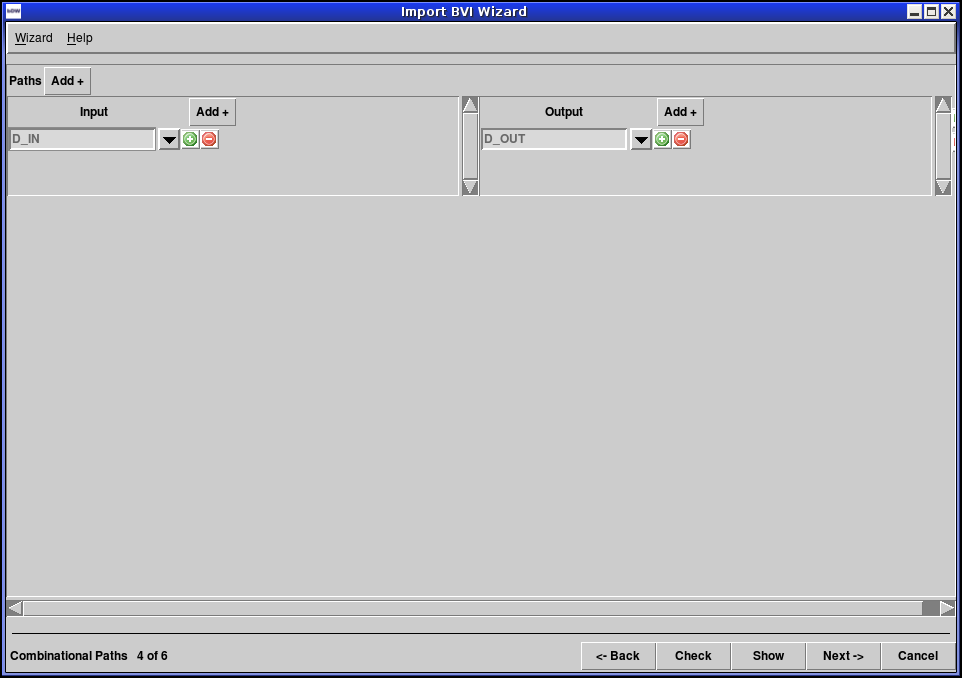
\includegraphics[width = 5 in]{figures/importbvi4}
\caption{Step 4: Combinational Paths }
\label{fig-importbvi4}
\end{center}
\end{figure}

Step 4 of the wizard, shown in Figure \ref{fig-importbvi4}, defines
the \te{path} statements.  A \te{path} statement indicates  a
combinational path
from the first port to the second port.  The compiler assumes
there will be a path from the input parameters of a \te{value} or an
\te{ActionValue} method to its result, so these need not be explicitly
specified.

The paths defined in the \te{path} statement are used by the compiler
in scheduling
and in checking for combinational cycles in a design.

To add the first path, use the \te{Add+} button. Then select the input
and output of the path from the drop down list boxes.

% -----

\subsubsection{Step 5: Scheduling Annotation}

\begin{figure}[htbp]
\begin{center}
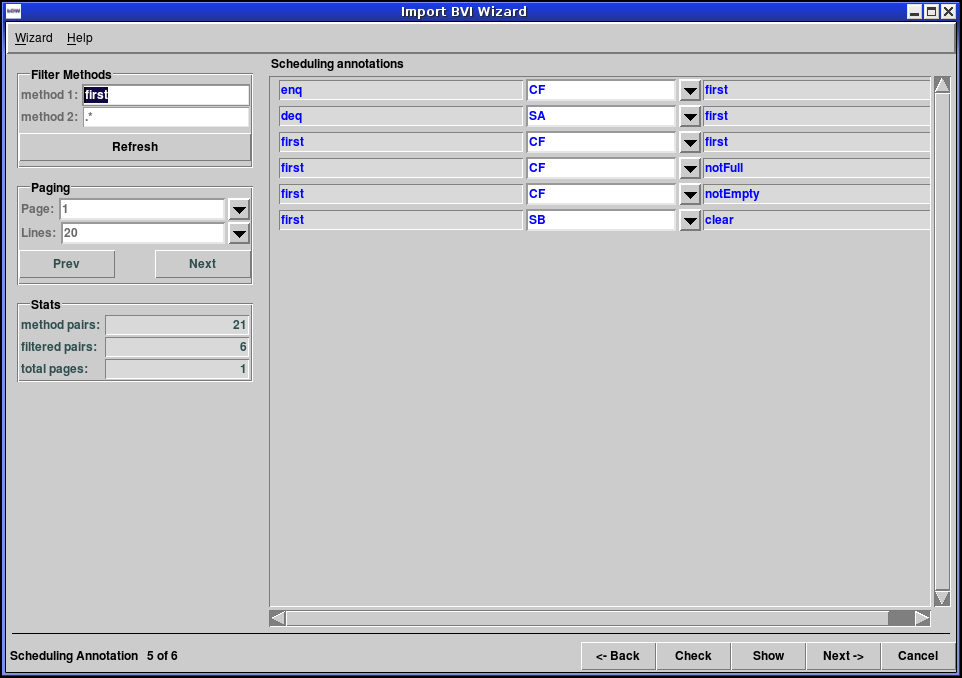
\includegraphics[width = 5 in]{figures/importbvi5}
\caption{Step 5: Scheduling Annotations }
\label{fig-importbvi5}
\end{center}
\end{figure}

Step 5 of the wizard, shown in Figure \ref{fig-importbvi5},  defines the scheduling constraints between the
methods of the module, as specified
by the \te{schedule} statements.

Each pair of methods can have only one relationship annotation.  Methods
clocked by unrelated clocks must have an relationship of \te{CF}.
%For methods clocked by related clocks the default is
%\texttt{C}.
The compiler generates a warning if an annotation between a method
pair is missing.

The wizard will list all the combinations of methods, with a default
scheduling annotation for each one.  To change the annotation, select
the correct value from the drop-down list box.

\begin{tabbing}
The m\=eanings of \= the operators are: \\
\\
\>\texttt{C} \>       conflicts \\
\>\texttt{CF} \>      conflict-free \\
\>\texttt{SB} \>     sequences before \\
\>\texttt{SBR} \>     sequences before, with range conflict (that is,
not  composable in parallel) \\
\>\texttt{SA} \>     sequences after \\
\>\texttt{SAR} \>     sequences after, with range conflict (that is,
not  composable in parallel) \\
\end{tabbing}

% -----

\subsubsection{Step 6: Finish}

\begin{figure}[htbp]
\begin{center}
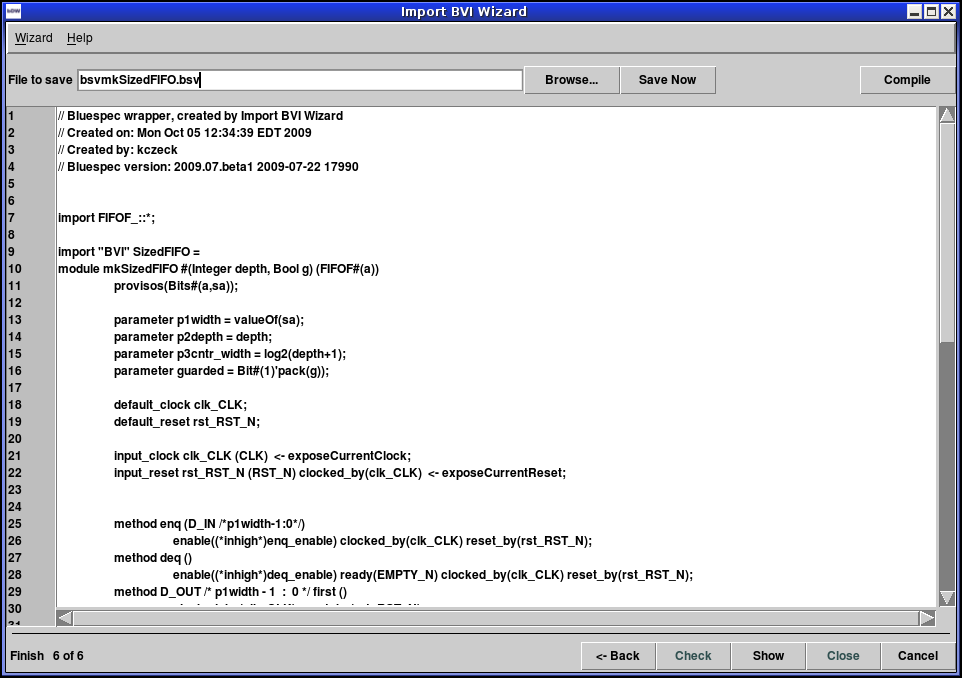
\includegraphics[width = 4 in]{figures/importbvi6}
\caption{Step 6: Finish }
\label{fig-importbvi6}
\end{center}
\end{figure}

The final window in the wizard, shown in Figure \ref{fig-importbvi6},  displays the  complete Verilog wrapper, including
the \te{import "BVI"} statement and any interfaces generated by the
wizard.  To compile the BSV code, select \te{Show} and then
\te{Compile}.   You must save the statement to a
file before closing the wizard or the information will be lost.

% ------------------------------------------------------------
% Appendices

\pagebreak

\appendix

% ------------------------------------------------------------

\section{Environment variables}
\index{environment variables}
\label{app-env}

The BSC tools allow customization through a large number of
environment variables that can be optionally set in the Unix shell.
Please refer to the BSC documentation for details.
BDW supports the following additional variables, which are all
optional.

% -------------------------

%\subsection{Workstation variables}

\index{BLUESPECTMP@\te{BLUESPECTMP}}
\index{environment variables!\te{BLUESPECTMP}}
\index{TMP@\te{TMP}}
\index{environment variables!\te{TMP}}
\index{TEMP@\te{TEMP}}
\index{environment variables!\te{TEMP}}
\index{EDITOR@\te{EDITOR}}
\index{environment variables!\te{EDITOR}}
\index{BROWSER@\te{BROWSER}}
\index{environment variables!\te{BROWSER}}

\begin{codebox}
BLUESPECTMP             locations for Workstation tmp files
TMP                     alternate for BLUESPECTMP
TEMP                    alternate for TMP
EDITOR                  editor used by Workstation
BROWSER                 command line to launch html browser used to display doc
\end{codebox}

The variable \te{BLUESPECTMP} specifies where temporary files generated
by the Workstation are stored, including wave files.  Since the Workstation
can use a wave viewer installed on a different machine, the temporary
files must be in a location that can be accessed by both machines.
\te{TMP} is an alternative variable for the tmp directory 
if \te{BLUESPECTMP} is not found, and \te{TEMP} is alternative if neither
of those is found.

% ------------------------------------------------------------

\section{Viewing graphs and installing Tcldot}
\label{graphviz-install}
\index{Tcldot}

% The compiler generates scheduling graphs during compilation when given
% the flag \te{-sched-dot}, from either the command line or the
% Workstation.  It creates several files named in the style
% \te{<Module>\_<GraphType>.dot}.

The Tcldot package is used by the BSC Development Workstation (BDW) to
display scheduling graphs.  

Note, the standalone Bluespec compiler (\te{bsc} command) does not depend
on Tcldot. When compiling with the flag \te{-sched-dot} the compiler
generates scheduling graph files which are
named in the following style: 

\begin{verbatim}
<Module>_<GraphType>.dot
\end{verbatim}

To view the generated scheduling graphs without the BDW, you 
can use any of a number of 3rd-party packages capable of displaying
\te{.dot} files. One example is  the
viewer application  called \te{dot}.  \te{dot} converts a \te{.dot}
file to a pdf or png format. 

To view the graphs from the BDW, you must
install Tcldot, which is an add-on to the graphviz package.
Unfortunately, a newer version of Tcldot (2.21 or greater) is required
than the one which come with the standard linux distributions.  Tcldot
can be downloaded from
\href{http://www.graphviz.org}{www.graphviz.org}.

To verify if Tcldot is installed, start a \te{Tcl/wish} shell to see
if and where Tcldot is available on your system.

\begin{itemize}
\item On a linux command line start \te{wish}:
\begin{verbatim}
linux>wish
\end{verbatim}
An empty wish window will pop-up. On the command line the wish shell
will have the tcl  command prompt \te{\%}.

\item Load the Tcldot package from the wish shell:
\begin{verbatim}
% package require Tcldot
\end{verbatim}
If installed, the version number will be returned.  The version must
be greater than 2.21.  If this step fails (\te{package not found}),
 Tcldot is not installed or not found in your path.
\item Verify where in tcl's search path Tcldot was found:
\begin{verbatim}
% puts $auto_path
\end{verbatim}
This will return tcl's search path.  Example:
\begin{verbatim}
/usr/share/tcltk/tcl8.5 /usr/lib /usr/local/lib/tcltk
/usr/local/share/tcltk /usr/lib/tcltk  /usr/lib/tcltk/graphviz
\end{verbatim}
You should find an obvious entry for graphviz.
\end{itemize}

To update the tcl search path in the BDW
\begin{itemize}
\item Create the file \te{\$\{HOME\}}/.bluetclrc
\item Add the following line to the \te{bluetclrc} file, using the
graphviz search path found above:
\begin{verbatim}
lappend auto_path /user/lib/tcltk/graphviz/
\end{verbatim}
\item Save the file and launch the Workstation
\end{itemize}


% Here
% are some instructions which we have used to install Tcldot on Linux
% Ubuntu v8.10.

% The package graphviz, \index{graphviz} including the Tcl extensions,
% can be installed
% to view the scheduling graphs in the Development Workstation. The
% graphviz package is not required to use the Development Workstation;
% it is required to view graphs from within the Development
% Workstation.  The graphviz
% Tcl extensions (Tcldot) \index{Tcldot} must be compatible with Tcl 8.5(Tcldot
% version 2.21 or greater) to work with the
% Development Workstation.  You may need to adjust the autopath for the
% graphvix package in the file \te{\$HOME/.bluetclrc} for your
% installation.    For more information on installing and using Tcl,
% refer to the many resources available on the web, including \href{http://www.tcl.tk/doc/}{www.tcl.tk}.

% To view the scheduling graphs without the Development Workstation, you
% can use any of a number of 3rd-party packages capable of displaying
% dot files, including the graphviz viewer application called \te{dot}, which
% converts a \te{.dot} file to a pdf or png format.  See
% \href{http://www.graphviz.org}{www.graphviz.org} for more information.

% ------------------------------------------------------------
% Appendix: BDW Tcl commands

% Include the 
% ------------------------------------------------------------
% ------------------------------------------------------------

\section{Bluetcl Reference}
\label{tcl-commands}

Bluetcl is a Tcl extension with a collection of scripts and packages 
providing an interface into the BSC view of a design.
You can execute Bluetcl commands and scripts from a
unix command line or from the command window in the Development
Workstation.

Bluetcl contains several layers (scripts, commands, packages) which
should be familiar to  the Tcl
programmer.  You can use Bluetcl extensions within Tcl scripts.
More information on Tcl is available at \te{www.tcl.tk} or
from the many books and references written about Tcl/Tk.

More information on Bluetcl can be found in the BSC documentation.

% ------------------------------------------------------------

\subsection{Invoking Bluetcl}

Bluetcl commands can be run either interactively or through Tcl
scripts.  These commands load, execute, and interact with
BSC-generated  files.   As with the Bluespec compiler,
pre-elaboration  information is obtained
from the \te{.bo} files, and post-elaboration information is
obtained from the \te{.ba} files.  

Bluetcl commands can be invoked in the following  ways.
\begin{itemize}
\item You can invoke Bluetcl from a unix prompt by typing
\te{bluetcl}.  This command provides a Tcl shell with the Bluetcl
extensions.
\item When in the BSC Development Workstation, the command window
provides a Bluetcl shell.
\item Finally, you can write and use Tcl scripts which use Bluetcl.
Examples can be found in the BSC repository.
\end{itemize}

% ------------------------------------------------------------

\subsection{Packages and namespaces}
\label{packages}
% All Bluetcl objects are defined in the namespace \te{Bluetcl}.
Bluetcl is organized into a collection of packages, which are
described in this appendix. The major packages are:
\begin{itemize}
\item The \te{Bluetcl} package which contains the low-level commands  to  interact with Bluespec files and designs.  
\item The \te{Bluesim} package containing Bluesim command extensions.\footnote{The  {\bf\tt sim} command for interacting with
Bluesim simulation objects (\te{.so} files) is contained in both the
\te{Bluetcl} and \te{Bluesim} packages.}
\item The WS package contains commands for interacting with the Workstation.
\end{itemize}

The  standard Tcl packages \te{Itcl}, \te{Itk}, and \te{Iwidgets} are
 available with Bluetcl  and can be used
 when creating  your own scripts.  

All commands in the \te{Bluetcl} package are in the \te{Bluetcl}
namespace.  All commands in the \te{Bluesim} package are in the
\te{Bluesim} namespace.   The commands in the \te{WS} package are
divided into multiple namespaces.

When referencing a command you must specify the namespace.  Example:
\begin{verbatim}
    Bluetcl::version
\end{verbatim}
Alternately, you can import commands from a namespace.  The following example
imports all the commands in a namespace:
\begin{verbatim}
    namespace import ::Bluetcl::*
\end{verbatim}
Or you can import a single command:
\begin{verbatim}
    namespace import ::Bluetcl::schedule
\end{verbatim}

Since the \te{WS} package contains multiple namespaces,  you must
specify the full namespace when referencing a \te{WS} command or
importing the commands from the namespace.  Example:
\begin{verbatim}
    WS::Build::link
    namespace import ::WS::Build::link
\end{verbatim}

Refer to the \te{Tcl} documentation for additional information on packages
and namespaces.

% ------------------------------------------------------------

\subsection{Customizing Bluetcl}
\label{custom}
\index{.bluetclrc}

You can use Bluetcl, along with all standard Tcl constructs, to
write scripts, issue commands, and customize the Development Workstation.
Bluetcl and the Development Workstation all source the setup
file \te{\$HOME/.bluetclrc} during initialization.  You can customize
Bluetcl and the Development Workstation by adding to 
 the \te{.bluetclrc} file.

% The Bluetcl interpreter is
% identical to the standard Tcl  interpreter with the
% following additions:
% \begin{itemize}
% \item It includes the Bluetcl packages
% \item The search paths are setup to look for other Bluespec
% extensions and customizations.
% \end{itemize}

The \te{namespace import} command can be put in the \te{.bluetclrc}
file, providing the command into the current namespace when the file
is sourced.  This will allow you to use just the command name in
scripts or from the command line.

% ------------------------------------------------------------

\subsection{Command Reference Conventions}

The next sections document the commands available from Bluetcl and
the Workstation (both general utilities and the Workstation code itself).
The following conventions are used within the command reference:
\begin{tabbing}
keywordandafew     \=     \kill
{\em name} \> identifier \\
{\bf keyword} \> as is \\
$[...]$ \> optional \\
%\{...\} \> repeated\\
\end{tabbing}

When an argument (or token) contains embedded spaces, the argument may
need to be enclosed in brackets (\te{\{ \}}).
% Note: For repeated arguments (\{ \}), one or more arguments may be
% specified. If only one item is specified, no brackets (\{ \}) should
% be used.  If multiple arguments are specified the list may be
% enclosed in brackets. 

% NOTE:I need a working example.  flag show seems to use a different syntax.
% Example:
% \begin{verbatim}
%      flag show sched-dot 
% This works differently - doesn't follow syntax
%      flag show sched-dot license-type p
% \end{verbatim}

% ------------------------------------------------------------

\subsection{General Bluetcl package command reference}

% -------------------------

\subsubsection{Bluetcl}

The commands in the \te{Bluetcl} package
provide a low-level interface to access BSC-specific files
(\te{.bo/.ba}) for use by Tcl programmers; they are not intended
for interactive use.  

Please refer to the BSC documentation for details on the
\te{Bluetcl} commands.

Before using a command from the \te{Bluetcl package},  the
following Tcl command must  be executed, either in a script, 
from the command line, or in the \te{.bluetclrc} file:
\begin{verbatim}
    package require Bluetcl
\end{verbatim}

All commands in the \te{Bluetcl} package are in the  \te{Bluetcl::}
namespace.  The namespace must be referenced, as described in Section
\ref{custom}, either by using the \te{namespace import} command or by
prepending the command name with \te{Bluetcl::}.  Example:
\begin{verbatim}
    Bluetcl::bpackage list
\end{verbatim}

% -------------------------

\subsubsection{Bluesim}

The \te{Bluesim} package contains the \te{sim} command which controls
Bluesim interactive mode.  This command is also found in the
\te{Bluetcl} package.

Please refer to the BSC documentation for details on the
\te{sim} command.

Before using a command from the Bluesim package,  the
following Tcl command must  be executed, either in a script, 
from the command line, or in the \te{.bluetclrc} file:
\begin{verbatim}
    package require Bluesim
\end{verbatim}

All commands in the \te{Bluesim} package are in the  \te{Bluesim::}
namespace.  The namespace must be referenced, as described in Section
\ref{custom}, either by using the \te{namespace import} command or by
prepending the command name with \te{Bluesim::}.  Example:
\begin{verbatim}
    Bluesim::sim clock
\end{verbatim}

% -------------------------

\subsubsection{Virtual}
\label{app-virtual}

The \te{Virtual} package provides Bluespec-specific accessor objects
 (virtual objects) including instantiation objects, signal objects,
 and method objects.  You  can select objects based on type, name, or
 relationship with other objects through 
 methods provided in the package.

With the \te{Virtual}  package you can:
\begin{itemize}
\item  Explore the elaborated design structure.
\item  Collect and filter the signals associated with specific
rules or submodules of a design.
\item Interact with a waveviewer object.
\item Perform these tasks in either batch or interactive mode.
\end{itemize}

Through  the design exploration capabilities of  the virtual
objects, signals associated with specific rules and instantiations can
be collected and output as a text file or  sent to a
waveform viewer.  

The term {\em virtual object} is used for two reasons:

\begin{itemize}
\item Although the objects appear to be fully populated at
  all times, the actual associated information is only obtained from
  the Bluespec database on an as-needed basis.  Caching
  mechanisms are used to avoid the need to obtain the same information
  multiple times.

\item Similarly, although objects appear  as true
  pointer-based objects, the actual implementation must conform to the
  capabilities of the \te{Tcl}  language with the \te{[incr Tcl]} (\te{iTcl})
  extensions. The \te{iTcl} package  adds   object-oriented
  programming constructs to \te{Tcl}. 
 Each object in the \te{Virtual} package is implemented as a \te{iTcl}
  class.  Information on \te{iTcl} can be 
  found at \te{www.incrtcl.sourceforge.net/itcl}

\end{itemize}

A number of the object methods select objects using   filter
patterns.  
The default pattern matching mechanism  is glob  unless the \te{-regexp} flag is
specified, specifying regular expressions. 




\subsubsubsection{inst (command)} 
\index[commands]{Virtual!inst}


The \te{inst} command provides access to the \te{inst} objects in the
current elaborated hierarchy tree.  Each object is of a defined
\te{kind}, where the values of \te{kind} are: 
\begin{itemize}
\item \te{Rule}:  Bluespec rules
\item \te{Prim}: imported Verilog IP, including common
BSC-provided primitives such as FIFOs
\item \te{Synth}:  module at the synthesis boundary
\item  \te{Inst}: not a \te{Rule}, \te{Prim}, or \te{Synth}
\end{itemize}

\begin{tabular}{|p {1.8 in}| p {3.8 in}|}
\hline
\hline
{\bf inst} {\bf top}& Returns  the top \te{inst} object or an error if
no modules have been loaded.\\
\hline
{\bf inst} {\bf filter} \te{[}{\bf -regexp}\te{]} & Returns a list of \te{inst} objects from the
current elaborated\\
   \te{[} {\bf -kind} {\em kind} \te{] [} {\bf
-nametype} {\bf bsv $\mid$ synth}\te{]} {\em pattern } & hierarchy
tree. A {\em pattern} must be specified. File
 glob matching is used for  name matching unless \te{-regexp} is
 specified, then regex is used. Optional  \te{-kind}, and \te{-nametype} flags 
 can be used to filter the results, where \te{kind} is either
 \te{Rule}, \te{Prim}, \te{Synth}, or \te{Inst} and \te{nametype}
 is either \te{bsv} or \te{synth}.  \\
\hline
\hline
\end{tabular}

{\bf Example: Using the \te{inst} command}
% Note:  The examples are generated using
% training/example/debug/DMA_ex1

The values returned from the commands are displayed in boxes.  Line
feeds have been added for clarity.


\begin{itemize}

\item   Set the
variable \te{demo} to the value returned by the \te{top} command.
\begin{verbatim}
   set demo [Virtual::inst top]
\end{verbatim}

\item Retrieve a list of the all \te{inst} objects from the
current elaborated hierarchy tree.
\begin{verbatim}
   Virtual::inst filter *
\end{verbatim}

\begin{codebox}
vInst0 vInst1 vInst2 vInst3 vInst4 vInst5 vInst6 vInst7 vInst8 vInst9
vInst10 vInst11 vInst12 vInst13 vInst14 vInst15 vInst16 vInst17
vInst18 vInst19 vInst20 vInst21 vInst22 vInst23 vInst24 vInst25
vInst26 vInst27 
\end{codebox}

\item  Display the bsv names of the \te{inst} objects. The
 \te{Virtual::omap} function is a convenience function to 
call the same method on a list of objects.  In this example, the
 method \te{name bsv} is being called for each \te{inst} returned by
 the \te{filter} method.
\begin{verbatim}
   Virtual::omap "name bsv" [Virtual::inst filter *]
\end{verbatim}

\begin{codebox}
mkDMA cnfReqF cnfRespF mmu1ReqF mmu1RespF mmu2ReqF mmu2RespF
dmaEnabledR readAddrR readCntrR currentReadR currentWriteR
portSrcDestR destAddrR responseDataF destAddrF startRead1 startRead2
finishRead1 finishRead2 startWrite1 startWrite2 finishWrite1
finishWrite2 markTransferDone writeConfig readConfig unknownConfig 
\end{codebox}

\end{itemize}


\subsubsubsection{VInst (virtual class)}

\te{VInst} is a virtual class in which  the 
\te{vinst} objects refer to  a specific instantiation in the
current elaborated hierarchy tree.

For name and path you must indicate whether you are querying the bsv
object or the synthesized object.  The name and path of an object may
be different in the BSV code and in the 
generated Verilog.  When querying for the object name and path, the
type of the object, as indicated by the
keyword \te{bsv} or \te{synth}, may be provided.  The default type is \te{bsv}.


\begin{tabular}{|p {1.8 in}| p {3.8 in}|}
\hline
\hline
{\em vinst} {\bf key}& Returns a unique identifier associated with this \te{vinst} object.\\
\hline
{\em vinst} {\bf kind}& Returns one of \te{Rule}, \te{Prim}, \te{Synth}, or \te{Inst}.\\
\hline
{\em vinst} {\bf name} \te{[}{\bf bsv $\mid$ synth}\te{]} & Returns the local
name of the instantiation, either from the bsv code or the generated
RTL.  The keyword \te{bsv} returns the name of 
the object in the BSV code while the keyword \te{synth} returns the
the  name  of the
instantiation of the object in the generated RTL.  \\
\hline
{\em vinst} {\bf path} \te{[}{\bf bsv $\mid$ synth}\te{]}& Returns the full path
name of the instantiation, either from the bsv code or the generated
RTL.  The keyword \te{bsv} returns the  path of 
the object in the BSV code while the keyword \te{synth} returns the
the  path of the
instantiation of the object in the generated RTL.  \\ 
\hline
{\em vinst} {\bf signals}& Returns a list of the
signal objects associated with the \te{vinst}.\\ % An optional \te{filter}
% argument can be used to filter the results based on a \te{signal}'s name or attributes.\\
\hline
 {\em vinst} {\bf parent}& Returns either the parent \te{vinst} object or an empty string. The top \te{vinst} does not have a parent.\\
 \hline
{\em vinst} {\bf children}& Returns a list of \te{vinst} objects.\\
\hline
{\em vinst} {\bf ancestors}&Returns a list of ancestors of the
 \te{vinst} object or an empty string.  The top \te{vinst} does not
 have any ancestors.\\
\hline
 {\em vinst} {\bf position}& Returns the position of the associated
 instantiation in the source BSV code.\\
\hline
{\em vinst} {\bf predsignals}& Returns a list of the rule predicate signals
 associated for a \te{vinst} of kind \te{Rule} or returns an empty string.\\
 \hline
{\em vinst} {\bf bodysignals}& Returns a list of the rule body signals
 associated for a \te{vinst} of kind \te{Rule} or returns an empty
 string. \\
 \hline
{\em vinst} {\bf predmethods}& Returns a list of the rule predicate methods
 associated for a \te{vinst} of kind \te{Rule} or returns an empty string.\\
 \hline
{\em vinst} {\bf bodymethods}& Returns a list of the rule body methods
 associated for a \te{vinst} of kind \te{Rule} or returns an empty
 string. \\
 \hline
{\em vinst} {\bf interface}&Returns a list of the interfaces
 associated with the \te{vinst} object.\\
\hline
% {\em vinst} {\bf module}& Returns the name of bsv module associated
% with the \te{vinst} object.\\
% \hline
 {\em vinst} {\bf portmethods}& Returns a list of all the 
 methods provided by  a \te{vinst} object
 of type \te{Prim} or \te{Synth}. \\
 \hline
{\em vinst} {\bf class}& Returns (for type checking) the {\em class} of the object (always \te{VInst}).\\
\hline
\hline
\end{tabular}

{\bf Example: Display all children}

Display the children of the top vinst, where the value of the vinst is
in the  variable \te{\$demo} (set in the previous example).

\begin{verbatim}
   $demo children
\end{verbatim}


\subsubsubsection{signal (command)}
\index[commands]{Virtual!signal}

This command provides access to the \te{signal} objects in the current
elaborated hierarchy tree and allows formatted signals to be sent to
waveform viewer or to a file for later use.

\begin{tabular}{|p {2.2 in}| p {3.4 in}|}
\hline
\hline
{\bf signal} {\bf filter}& Returns a list of \te{signal} objects from the current\\
\te{[}{\bf -inst} {\em objects} {\bf ]} \te{[}{\bf -regexp} \te{]} {\em
pattern} \te{[}{\bf -nametype} {\bf bsv $\mid$ synth}\te{]} &elaborated hierarchy tree.   The optional \te{-inst} flag specifies which
hierarchies to search.  A {\em pattern} must be specified.  File globs are used for pattern matching unless
\te{-regexp} is specified before the pattern, then regex is used.\\ 
 \hline
%   {\bf signal} {\bf add} {\em filestream} {\em signals}& Writes a list of signal objects formatted for a waveform \\
%   {\bf[ Novas\te{|}GtkWave]} {\bf[ typed\te{|}bits]}& viewer to an opened Tcl filestream.\\
\hline
\hline
\end{tabular}

{\bf Example: Using \te{signal filter}}
\begin{itemize}


\item Use the pattern \te{*} to return all signals.

\begin{verbatim}
   Virtual::signal filter *
\end{verbatim}

\begin{codebox}
vSignal0 vSignal1 vSignal2 vSignal3 vSignal4 vSignal5 vSignal6
vSignal7 vSignal8 vSignal9 vSignal10 vSignal11 vSignal12 vSignal13
vSignal14 vSignal15 vSignal16 vSignal17 vSignal18 vSignal19 vSignal20
vSignal21 vSignal22 vSignal23 vSignal24 vSignal25 vSignal26 vSignal27
vSignal28 vSignal29 vSignal30 vSignal31 vSignal32 vSignal33 vSignal34
vSignal35 vSignal36 vSignal37 vSignal38 vSignal39 vSignal40 vSignal41
vSignal42 vSignal43 vSignal44 vSignal45 vSignal46 vSignal47 vSignal48
vSignal49 vSignal50 vSignal51 vSignal52 vSignal53 vSignal54 vSignal55
vSignal56 vSignal57 vSignal58 vSignal59 vSignal60 vSignal61 vSignal62
vSignal63 vSignal64 vSignal65 vSignal66 vSignal67 vSignal68 vSignal69
vSignal70 vSignal71 vSignal72 vSignal73 vSignal74 vSignal75 vSignal76
vSignal77 vSignal78 vSignal79 vSignal80 vSignal81 vSignal82 vSignal83
vSignal84 vSignal85 vSignal86 vSignal87 vSignal88 vSignal89 vSignal90
vSignal91 vSignal92 vSignal93 vSignal94 vSignal95 vSignal96 vSignal97
vSignal98 vSignal99 vSignal100 vSignal101 vSignal102 vSignal103
vSignal104 vSignal105 vSignal106 vSignal107 vSignal108 vSignal109
vSignal110 vSignal111 vSignal112 vSignal113 vSignal114 vSignal115
vSignal116 vSignal117 vSignal118 vSignal119 vSignal120 vSignal121
vSignal122 vSignal123 vSignal124 vSignal125 vSignal126 vSignal127
vSignal128 vSignal129 vSignal130 vSignal131 vSignal132 vSignal133
vSignal134 vSignal135 vSignal136 vSignal137 vSignal138 vSignal139
vSignal140 vSignal141 vSignal142 vSignal143 vSignal144 vSignal145
vSignal146 vSignal147 vSignal148 vSignal149 vSignal150 vSignal151
vSignal152 vSignal153 vSignal154 vSignal155 vSignal156 vSignal157
vSignal158 vSignal159 vSignal160 vSignal161 vSignal162
\end{codebox}

\item Display only the \te{WILL\_FIRES} signals
\begin{verbatim}
   Virtual::signal filter WILL*
\end{verbatim}

\begin{codebox}
vSignal139 vSignal141 vSignal143 vSignal145 vSignal147 vSignal149
vSignal151 vSignal153 vSignal155 vSignal157 vSignal159 vSignal161 
\end{codebox}
\end{itemize}

% Filtering the CAN\_FIRES only under the object \te{::Vo::<inst\_19>}
% \begin{verbatim}
% % Virtual::signal filter -name CAN* -inst ::Vo::<inst_19>
% \end{verbatim}

% \begin{codebox}
% ::Vo::<signal_15>
% \end{codebox}

\subsubsubsection{VMethod (virtual class)}

The
\te{vmethod} objects  describe the methods in the current 
elaborated hierarchy. 

\begin{tabular}{|p {1.8 in}| p {3.8 in}|}
\hline
\hline
{\em  vmethod} {\bf inst}& Returns the associated \te{inst} object.\\
\hline
{\em vmethod} {\bf name}& Returns the local name of the vmethod.\\
\hline
 {\em vmethod} {\bf position}& Returns the position of the associated
 \te{inst} in the source BSV code.\\
\hline
{\em vmethod} {\bf path} {\bf bsv $\mid$ synth}& Returns the full path
name of the instantiation, either from the bsv code or the generated
RTL.  The keyword \te{bsv} returns the  path of 
the method in the BSV code while the keyword \te{synth} returns the
the  path of the
instantiation of the method in the generated RTL.  \\ 
\hline
{\em vmethod} {\bf signals}& Returns a list of the
signal objects associated with the \te{vmethod}.\\ 
\hline
{\em vmethod} {\bf class}& Returns (for type checking) the {\em class}
of the object (always \te{VMethod}).\\
\hline
\hline
\end{tabular}


\subsubsubsection{VSignal (virtual class)}

The \te{vsignal} objects describe the  signals in the current 
elaborated hierarchy. 

\begin{tabular}{|p {1.8 in}| p {3.8 in}|}
\hline
\hline
{\em  vsignal} {\bf key}& Returns a unique identifier associated with
this \te{vsignal} object.\\ 
\hline
{\em vsignal} {\bf kind}& Returns one of %\te{Input},
                                %\te{Output},\te{Clock}, 
\te{WillFire}, \te{CanFire}, or \te{Signal}.\\
\hline
{\em vsignal} {\bf name}& Returns the local name of the vsignal.\\
\hline
{\em vsignal} {\bf path} [{\bf bsv $\mid$ synth}] & Returns the full path name of the vsignal.\\
\hline
{\em vsignal} {\bf type}& Returns the BSV type of the signal.\\
\hline
{\em vsignal} {\bf inst}& Returns the associated \te{inst} object.\\
\hline
 {\em vsignal} {\bf position}& Returns the position of the associated
 \te{inst} in the source BSV code.\\
\hline
% {\em vsignal} {\bf methods}& Returns a list of all the methods associated with the \te{signal} object.\\
%\hline
{\em vsignal} {\bf class}& Returns (for type checking) the {\em class}
of the object (always \te{VSignal}).\\
% \hline
% {\em vsignal} {\bf wave\_format}& Generates the signal type and signal
% name in a format understood by the waveform viewer (\te{Waves::send\_typed\_signals}).\\ 
\hline
\hline
\end{tabular}

\subsubsubsection{reset (command)} 
\index[commands]{Virtual!reset}

\begin{tabular}{|p {1.8 in}| p {3.8 in}|}
\hline
\hline
{\bf reset}& Deletes all existing virtual objects.  This command is
called automatically when a new \te{.ba} file is loaded.\\
\hline
\hline
\end{tabular}

\subsubsubsection{omap (command)} 
\index[commands]{Virtual!omap}

\begin{tabular}{|p {1.8 in}| p {3.8 in}|}
\hline
\hline
{\bf omap}& Maps a function over a series of objects. \\
\hline
\hline
\end{tabular}


{\bf Example: Mapping the \te{name synth} command over the \te{inst filter *}}

\begin{verbatim}
   Virtual::omap "name synth" [Virtual::inst filter *]
\end{verbatim}
\begin{codebox}
cnfReqF cnfRespF mmu1ReqF mmu1RespF mmu2ReqF mmu2RespF dmaEnabledR
readAddrR readCntrR currentReadR currentWriteR portSrcDestR destAddrR
responseDataF destAddrF RL_startRead1 RL_startRead2 RL_finishRead1
RL_finishRead2 RL_startWrite1 RL_startWrite2 RL_finishWrite1
RL_finishWrite2 RL_markTransferDone RL_writeConfig RL_readConfig
RL_unknownConfig 
\end{codebox}

{\bf Example: Using  virtual objects from the Workstation}

In this example we use  virtual objects to select and display
signals on the waveform viewer.
To use the \te{Virtual} package from within the Workstation, enter the Tcl
 commands in the command window of the Workstation.   Before entering
 commannds you must bring in the \te{Virtual} package:

\begin{verbatim}
   package require Virtual
\end{verbatim}

If you optionally import all the commands from the  \te{Virtual} package you
won't have to specify the full namespace each time you reference a
command from the package:

\begin{verbatim}
   namespace import Virtual::*
\end{verbatim}


\begin{itemize}
\item Build the design and load the waveform viewer (same as with any design)

\begin{itemize}
\item Within the Workstation, load the project file, build and
simulate the design while generating a waveform dump file.

\item Open the module browser, load the top module, start and attach
the waveform viewer and load the dump file.
\end{itemize}

\item Enter the Tcl commands  in the command window of  the
Workstation.

\begin{itemize}
\item  Load and import the Virtual package
\begin{verbatim}
   package require Virtual
   namespace import Virtual::*
\end{verbatim}

\item Select all the WILL\_FIRE signals
\begin{verbatim}
   set w [signal filter WILL_FIRE*]
\end{verbatim}

\item Display the names of the WILL\_FIRE signals

\begin{verbatim}
   omap name $w
\end{verbatim}

\end{itemize}



The \te{WILL\_FIRE} signals for the  design are displayed.

\begin{codebox}
WILL_FIRE_RL_startRead1 WILL_FIRE_RL_startRead2
WILL_FIRE_RL_finishRead1 WILL_FIRE_RL_finishRead2
WILL_FIRE_RL_startWrite1 WILL_FIRE_RL_startWrite2
WILL_FIRE_RL_finishWrite1 WILL_FIRE_RL_finishWrite2
WILL_FIRE_RL_markTransferDone WILL_FIRE_RL_writeConfig
WILL_FIRE_RL_readConfig WILL_FIRE_RL_unknownConfig
\end{codebox}

\item Send the \te{WILL\_FIRE} signals to the opened wave viewer.

\begin{codebox}
   set v [WS::Wave::clone_viewer]
   $v send_objects $w
\end{codebox}

\end{itemize}



\subsubsubsection{Using Virtual objects from the command line}


                   

\begin{itemize}
\item Start bluetcl and load the top module,  \te{mkTb} in this example.  \te{rlwrap} adds
readline editing and command history.  

\begin{verbatim}
rlwrap bluetcl

   Bluetcl::flags set "-sim"
   Bluetcl::module load mkTb
\end{verbatim}

\item Load the \te{Virtual} package and set the variable \te{\$top}
equal to the top of the instance.

\begin{verbatim}
   package require Virtual
   namespace import Virtual::*
   set top [inst top]
\end{verbatim}
\begin{codebox}
vInst58
\end{codebox}

\item List the children of  the module stored in the variable
\te{\$top}.

\begin{verbatim}
   $top children
\end{verbatim}
\begin{codebox}
vInst59 vInst60 vInst61 vInst62 vInst63 vInst64 vInst65 vInst66 vInst67
\end{codebox}

\item The names listed are not very informative.  List the bsv
module name for each of the children.  

\begin{verbatim}
   foreach k [$top children] { puts [$k name bsv] }
\end{verbatim}
\begin{codebox}
initiator_0
initiator_1
target_0
target_1
dut
mkConnection
mkConnection
mkConnection
mkConnection
\end{codebox}

\item The \te{Virtual::omap} function is a convenience function to
call the same method on a list of objects.  It does approximately the
same thing as the foreach above, without  the newlines.

\begin{verbatim}
   omap "name bsv" [$top children]
\end{verbatim}
\begin{codebox}
initiator_0 initiator_1 target_0 target_1 dut mkConnection mkConnection 
mkConnection mkConnection
\end{codebox}


\item The \te{"name bsv"} class method returns the name of the objects
in the inst.   You can use a filter  to return only a certain
instances. 

\begin{verbatim}
   omap "name bsv" [inst filter *]
\end{verbatim}
\begin{codebox}
mkTb initiator_0 rand32 r reqs resps expected_resps_0 expected_resps_1
gen_reqs accept_resps_from_0 accept_resps_from_1 initiator_1 rand32 r
reqs resps expected_resps_0 expected_resps_1 gen_reqs
accept_resps_from_0 accept_resps_from_1 target_0 reqs resps respond
target_1 reqs resps respond dut from_initiator_0 from_initiator_1
to_initiator_0 to_initiator_1 to_target_0 to_target_1 from_target_0
from_target_1 initiator_0_to_target_0 initiator_1_to_target_0
initiator_0_to_target_1 initiator_1_to_target_1
target_0_to_initiator_0 target_1_to_initiator_0
target_0_to_initiator_1 target_1_to_initiator_1 mkConnection
ClientServerRequest_0 ClientServerResponse_0 mkConnection
ClientServerRequest_1 ClientServerResponse_1 mkConnection
ClientServerRequest_2 ClientServerResponse_2 mkConnection
ClientServerRequest_3 ClientServerResponse_3 
\end{codebox}

\item  Filter the above list to show only the Rules.  You can also
filter on \te{Prim, Synth, and Inst}.

\begin{verbatim}
   omap "name bsv" [inst filter * -kind Rule]
\end{verbatim}
\begin{codebox}
gen_reqs accept_resps_from_0 accept_resps_from_1 gen_reqs
accept_resps_from_0 accept_resps_from_1 respond respond
initiator_0_to_target_0 initiator_1_to_target_0
initiator_0_to_target_1 initiator_1_to_target_1
target_0_to_initiator_0 target_1_to_initiator_0
target_0_to_initiator_1 target_1_to_initiator_1 ClientServerRequest_0
ClientServerResponse_0 ClientServerRequest_1 ClientServerResponse_1
ClientServerRequest_2 ClientServerResponse_2 ClientServerRequest_3
ClientServerResponse_3 
\end{codebox}


% \item Set a variable called \te{dut}
% \begin{verbatim}
% % set dut [Virtual::inst filter * -path /main/top/dut -nametype synth]
% \end{verbatim}
% \begin{codebox}
% ::Vo::<inst_6>
% \end{codebox}

\item Find all signals and list by name (results not listed here).
\begin{verbatim}
   omap name [signal filter *]
\end{verbatim}

\item  Find all \te{WILL\_FIRE} signals and list by name (results not
listed here)

\begin{verbatim}
   omap name [signal filter WILL_FIRE*]
\end{verbatim}

\item To save the signals in a GtkWave or NovasRC file format, use the
\te{Waves} package (Section \ref{app-Waves}).
In this example we define a viewer \te{v} that is a NovasRC viewer.

\begin{verbatim}
   package require Waves
   set v [Waves::start_replay_viewer -e mkTb 
                                    -backend -sim 
                                    -viewer NovasRC 
                                    -ScriptFile x1.rc ]
\end{verbatim}

\begin{codebox}
Opening x1.rc for NovasRC script capture
novasRC1
\end{codebox}

\item Send all the \te{WILL\_FIRE} signals to the script file
\te{x1.rc}.  From the Novas viewer you will be able to load the
signals saved in the 
\te{x1.rc} file.  With the \te{Waves} package you can format, send,
and save signals to waveform and script files.
\begin{verbatim}
   $v send_objects [signal filter WILL_FIRE*]
\end{verbatim}

\end{itemize}

% -------------------------

\subsubsection{Waves}

\label{app-Waves}

The \te{Waves} package manages
waveviewer objects.  A waveviewer  is an \te{iTcl} object associated
with a specific waveform viewer instance or a waveform viewer script
file.  The \te{Waves} package contains methods and commands to  
 create   waveviewer objects and then  format,  and send
signals to those  objects.  The package also contains a scripting
functionality to  create waveviewer
script files, an executable Tcl file containing wave history
data. Waveform scripts  can be run
interactively through a waveform viewer or in batch from a command
line, for testing and verification of  designs.


To use any of the objects in the \te{Waves} package, the package
must be loaded.

\begin{verbatim}
     package require Waves
\end{verbatim}

  

You first  define a  viewer
instance which is associated with a particular waveform viewer or
waveform viewer script file.  Supported viewer types  are: \te{Novas} and \te{GtkWave}
along with their associated 
script file formats: \te{NovasRC} and \te{GtkWaveScript}.  Both the
\te{create\_viewer} and  \te{start\_replay\_viewer} commands will
define a  viewer object;  the \te{start\_replay\_viewer} 
also sets the path and opens a \te{.ba} file, assigning the viewer
object to a specific design.  

Once you have defined a viewer object, use the \te{WaveViewer} methods to
 send objects to the viewer. 
  Sent objects may be virtual
signals, instances, and methods created using the \te{Virtual}
package, described in Section \ref{app-virtual}.


\subsubsubsection{WaveViewer commands}

%\subsubsubsection{set\_nonbsv\_hierarchy (command)} 
\index[commands]{Waves!set\_nonbsv\_hierarchy}
\index[commands]{Waves!get\_nonbsv\_hierarchy}
\index[commands]{Waves!create\_viewer}

\begin{tabular}{|p {1.8 in}| p {3.8 in}|}
\hline
\hline
{\bf create\_viewer} {\em class } [{\em args}]&   Defines a virtual
viewer object of the type specified by \te{class}. The valid values for
\te{class} are \te{Novas}, \te{GtkWave}, \te{NovasRC}, and
\te{GtkWaveSript}.  The optional \te{args}  are
shown in Figure \ref{Wavestcl} and the table below.\\
\hline
{\bf start\_replay\_viewer} [{\em args}] & Defines a virtual viewer
object ready to use on a specific design (sets the path and opens the
\te{.ba} file.)  The optional \te{args}  are
shown in Figure \ref{Wavestcl} and the tables below.   Refer to the
\te{WaveViewer} section for more options.\\
\hline
{\bf set\_nonbsv\_hierarchy} {\em hierarchy}&Sets the Verilog
hierarchy as default for all new viewers.  The default is \te{/main/top}. \\
\hline
{\bf get\_nonbsv\_hierarchy}&Returns the value of the Verilog hierarchy. \\
\hline
\hline
\end{tabular}

The abstract class in the package is the \te{WaveViewer} class hierarchy.  The classes \te{Viewer}
and \te{ScriptFile} define specific types of viewers and inherit  the
methods and attributes defined in the  \te{WaveViewer} class, 
  shown in Figure \ref{Wavestcl}.  Additional arguments,
specific to either viewers or script files, are defined in those
respective classes.


\subsubsubsection{Configure arguments}

The \te{iTcl} \te{configure} method provides access to public variables as
 configuration options and a method for setting  values of the
 variables.  These variables can also be modified when a replay
 script is run or the \te{start\_replay\_viewer} method is called.
The following  arguments are used by the
\te{configure} method to configure the waveviewer.  The table is divided
into sections by classes.  The \te{WaveViewer} arguments are used by
all classes, while the \te{Viewer} and \te{ScriptFile} arguments are used
by their respective classes. 


\begin{figure}[htb]
\begin{center}
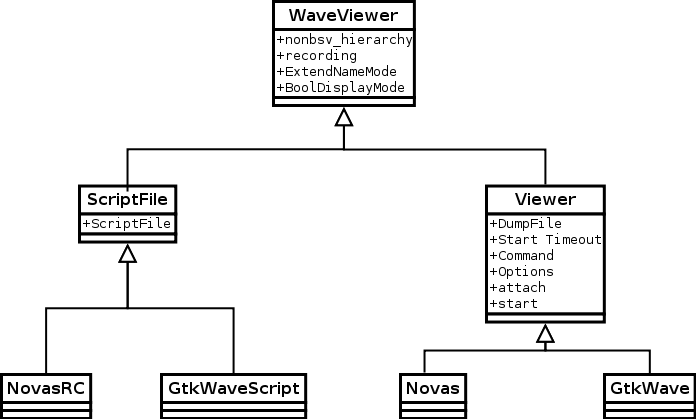
\includegraphics[width = 5 in]{figures/Wavestcl}
\caption{Inheritance of WaveViewer Class}
\label{Wavestcl}
\end{center}
\end{figure}





\begin{tabular}{|p {2.0 in}| p {3 in}|p{.6in}|}
\hline

\multicolumn{3}{|c|}{Configure arguments}\\
\hline

Argument&Description&Default  \\
\hline\hline
\multicolumn{3}{|l|}{ Arguments for all WaveViewer classes}\\
\hline
\hline
 \te{-nonbsv\_hierarchy} {\em path}&  Verilog hierarchy &\te{/main/top}\\

%\hline
 \te{-ExtendNameMode} {\bf true$\mid$false}&Determines how names are displayed in the viewer&
 false \\
%\hline
\te{-BoolDisplayMode} {\bf true$\mid$false} &Display Boolean as enum (true/false) or as 1/0 &false \\
%\hline 
\te{-recording} {\bf true$\mid$false}&If true,  commands are always recording &true\\
\hline
 \multicolumn{3}{|l|}{Arguments for Viewer classes (Novas and GtkWave)}\\
 \hline
\te{-DumpFile} {\em file}&Name of the dump file&\\
%\hline
\te{-StartTimeout} {\em time}&Delay after starting before declaring a timeout
 (Specific to viewer).  The {\em time} is an Integer.&20\\
%\hline
\te{-Command} {\em command}&Command to start viewer&\\
%\hline
\te{-Options} {\em options} &Command line options provided to viewer&\\

\te{-start} [{\bf 0} $\mid$ {\bf 1}]& Starts the wave viewer &0\\
\te{-attach} {\em viewer} &Attaches to the viewer& \\
\hline
 \multicolumn{3}{|l|}{Arguments for ScriptFile classes (NovasRc and GtkWaveScript)}\\
 \hline
\te{-ScriptFile} {\em file} & Specifies the name of the script file.&\\
\hline
\hline
\end{tabular}


\subsubsubsection{WaveViewer methods} 

\te{WaveViewer} is a virtual class in which the \te{viewer} objects
 refer to a specific instantiation of a
 waveform viewer or script file object.   
The  methods allow you to  configure, control, and query the \te{viewer}
 object.   You can send virtual objects and signals directly to the
 the viewer or   save the wave history  as a \te{.tcl} script file.



\begin{tabular}{|p {1.8 in}| p {3.8 in}|}
\hline
\hline
{\em viewer} {\bf configure} {\em args} & Uses the \te{iTcl}
\te{configure} method to set the configuration options.\\
\hline
{\em viewer} {\bf start} {\em args}& Starts the wave viewer object with the
provided {\em args}.  The arguments are listed in the \te{Configure
Arguments} table.\\
\hline
{\em viewer} {\bf isRunning}&Returns \te{true} if the wave viewer object is running.\\
\hline
{\em viewer} {\bf attach} {\em waveviewer} &Attaches the selected wave viewer
object.  If empty, detaches.\\
\hline
{\em viewer} {\bf close}&Closes the selected wave viewer object.\\
\hline
{\em viewer} {\bf load\_dump\_file} {\em filename} & Loads the file
{\em filename}
into the wave viewer object.\\
\hline
{\em viewer} {\bf reload\_dump\_file} &Reloads the current dump file.\\
\hline
{\em viewer} {\bf dump\_file\_loaded}&Returns \te{true} if the dump file is loaded. \\
\hline
{\em viewer} {\bf send\_objects} {\em objects}& Sends  virtual objects of type
\te{VInst}, \te{VSignal}, or \te{VMethod}  to the wave viewer object.\\
\hline
{\em viewer} {\bf send\_instance} {\em vinst} [{\em modifier}] & Sends an instance
object with a modifier to the wave viewer object.  The valid values of
\te{modifier} are \te{CLK, QOUT, CANFIRE, WILLFIRE, ALL, PREDICATE,
BODY}.  The default is \te{ALL}. \\
\hline
{\em viewer} {\bf send\_signals} {\em signal} & Sends the signal name (string of
the Verilog name) to the wave viewer.\\
\hline
{\em viewer} {\bf save\_history} {\em filename} &Saves the wave send history to a
tcl script file (\te{.tcl}) \\
\hline
{\em viewer} {\bf replay\_history\_file} {\em filename} & Replays the script file on
the wave viewer, sourcing the waveviewer script file without creating
a \te{wave\_history} file.\\
\hline
 {\em viewer} {\bf replay\_history\_list} {\em history\_list} &Replays the history
list. When a waveviewer script file is sourced it creates  a list variable named
\te{wave\_history}. Use  this method to replay the \te{wave\_history} file.\\
\hline
\hline
\end{tabular}




\subsubsubsection{WaveViewer script file}
\index{script file}


 The waveviewer script file is an
executable Tcl (\te{.tcl}) file containing wave history data. 
  The script file contains a list of
\te{wave\_history} elements where  each  element is comprised of  a
tag, a name, and a 
code value.  The tags are described in the table below.  The name is
the signal name and  can
contain  wildcards allowing signals to be selected dynamically when the file is
sourced or executed.  The data in the code value is based on the type
of signal.   The file  can be edited or
manipulated by the user in a text editor. 

The script file is created through the \te{save\_history} method.  You
can replay the script file using \te{replay\_history\_file}, which
will source the \te{.tcl} file and display the wave history on the
specified viewer instance.   You can also source the \te{.tcl} file 
from a bluetcl shell, creating a list variable named
\te{wave\_history} and then    replay the saved \te{\$wave\_history}
file through the \te{replay\_history\_list} method.


\begin{tabular}{|p{1 in}|p{4.5in}|}
\hline
\multicolumn{2}{|c|}{WaveViewer Script File Tags}\\
\hline
Tag& Signal Description\\
\hline \hline
\te{VSignal}& \te{VSignal}  object generated by the \te{Virtual}
class. \\
\hline
\te{SSignal} &Simple signal name.\\
\hline
\te{TSignal}&Simple signal name where the type is stored in the code value.\\
\hline
\te{VInst}&\te{VInst} object generated by the \te{Virtual} class.\\
\hline
\end{tabular}


The following options, in addition to the configure options,  are used when running the replay script or the
\te{start\_replay\_viewer} method.


\begin{tabular}{|p {1.8 in}|p{3.8in}|}
\hline
\multicolumn{2}{|c|}{Options for running  replay script and
\te{start\_replay\_viewer} method}\\ 
% \hline
% Option&Description  \\
\hline\hline
\te{-help} & Lists the options for the method  \\
\te{-p} {\em path}& Sets the Bluespec search path\\
\te{-e} {\em module}& Specifies the top  module\\
\te{-backend} [{\bf -verilog $\mid$ -sim}]& Specifies Verilog or Bluesim
as the backend, defaults to -verilog if left blank.\\

\te{-viewer} {\em class}&Sets the viewer class.   The valid values
for \te{class} are \te{Novas}, \te{GtkWave}, \te{NovasRC}, and
\te{GtkWaveSript}.\\
\hline
\hline

\end{tabular}



The script file can be either executed in a Unix shell or sourced in a
Tcl shell.   Executing the
script file from a Unix shell will execute the
following steps:
\begin{enumerate}
\item Load the \te{.ba} files (this may take some time)
\item Start the viewer
\item Execute the history
\item Exit
\end{enumerate}

\subsubsubsection{Example:  Creating and executing a viewer script file}

\begin{itemize}

\item Start bluetcl.  The command line in the Workstation is also a
bluetcl shell.

\begin{verbatim}
rlwrap bluetcl
\end{verbatim}

\item Load the \te{Virtual} and \te{Waves} packages.

\begin{verbatim}
   package require Virtual
   package require Waves
\end{verbatim}

\item Define the viewer and name it \te{v}

\begin{verbatim}
   set v [Waves::start_replay_viewer -e mkTb 
                                    -backend -sim 
                                    -viewer NovasRC 
                                    -ScriptFile x1.rc ]
\end{verbatim}

\begin{codebox}
Opening x1.rc for NovasRC script capture
novasRC1
\end{codebox}

\item Set the variable \te{r} to all rules where the name ends in 1

\begin{verbatim}
   set r [Virtual::inst filter -kind Rule *1]
\end{verbatim} 

\begin{codebox}
vInst17 vInst26 vInst44 vInst45 vInst48 vInst49 vInst52 vInst53
\end{codebox}

\item These are the instance names.  Let's view the BSV names
\begin{verbatim}
   Virtual::omap "name bsv" $r
\end{verbatim}

\begin{codebox}
accept_resps_from_1 accept_resps_from_1 initiator_0_to_target_1
initiator_1_to_target_1 target_0_to_initiator_1
target_1_to_initiator_1 ClientServerRequest_1 ClientServerResponse_1 
\end{codebox}

\item Send the objects in \te{\$r} to  to the viewer file \te{\$v} (\te{x1.rc})
\begin{verbatim}
   $v send_objects $r
\end{verbatim}

\item Save the session as a \te{WaveViewer} (\te{.tcl)} script file
\begin{verbatim}
   $v save_history x1.tcl
\end{verbatim}
\end{itemize}

\subsubsubsection{Example: Replaying a script on a waveform viewer}

\begin{itemize}
\item Start bluetcl and load the \te{Virtual} and \te{Waves} packages

\item Define a Novas viewer 

\begin{verbatim}
   set v1 [Waves::start_replay_viewer -e mkTb -backend -sim -viewer Novas]
\end{verbatim}

\item Start the viewer and load the dump file
\begin{verbatim}
   $v1 start
   $v1 load_dump_file dump.vcd
\end{verbatim}

\item Souce the \te{x1.tcl} file created in the previous example.
This will create the file \te{wave\_history}.
\begin{verbatim}
   source x1.tcl
\end{verbatim}

\item Replay the wave history

\begin{verbatim}
   $v1 replay_history_list $wave_history
\end{verbatim}

\item The waves will be displayed on the waveform viewer.

\end{itemize}

\subsubsubsection{Example: Loading a saved waveform file from within
the Workstation}

With a saved waveform files you can easily save and load a set of
signals through multiple iterations of a design, easily comparing
changes from one iteration to the next.

To load the saved signal files (\te{x1.rc})  using the Workstation:
\begin{itemize}
\item Open the design in the Workstation

\item Open the Module Browser

\item {\bf Load} top module

\item {\bf Start} the waveform viewer

\item {\bf Load} the dump file

\item From the waveviewer, restore signal ({\bf File $\rightarrow$ 
Restore Signal} in Novas).  Select the saved signals (\te{x1.rc}).

\item The waves will be displayed on the waveform viewer.
\end{itemize}

The above steps could all be done from a bluetcl command line, within
or outside of the Workstation.

% \subsubsection{Executing a \te{WaveViewer} script file}

% In the example above, we saved our session as a script file named
% \te{x1.tcl}.  

% \begin{enumerate}

% \end{enumerate}

% ------------------------------------------------------------

\subsection{Workstation package command reference}
 The \te{WS} package provides a
programming interface  to customize
the Workstation.  Specifically,  commands available from the Workstation menus
and toolbars can be executed from the Workstation command line or  included in \te{Tcl} scripts which are executed
from the Workstation.   These commands are only available in the
Workstation.  Attempting to use them in Bluetcl will
result in an error.

Tcl scripts using \te{WS} commands must be added to the
\index{.bluetclrc} \te{.bluetclrc} file. 

The \te{WS} package is divided into several sub-namespaces.  To execute a command
you must either specify the full path, including the package and
namespace, or import the namespace before executing the command.

For example, to execute the link command, in the Workstation command
line you would type:
\begin{verbatim}
    WS::Build::link
\end{verbatim}

Or, you could import the \te{Build} namespace, then execute the
command:
\begin{verbatim}
    namespace import ::WS::Build::*
    link
\end{verbatim}
The namespace only has to be imported once in a session.  After it has been imported, you can execute any of the
commands in the namespace without providing the full path name.
The \te{Tcl} documentation provides additional information on using namespaces.

% -------------------------

\subsubsection{WS::}

The \te{WS} namespace contains the \te{help} and
\te{change\_font\_size} commands.  

Example: Using help
\begin{verbatim}
    WS::help
    WS::help -command reload_packages
\end{verbatim}

Example: Increasing the font size by 1 point
\begin{verbatim}
    WS::change_font_size +1
\end{verbatim}


\index[commands]{WS!help}
\begin{tabular}{|p {2.2 in}| p {3.4 in}|}
\hline
\hline
{\bf help} &Displays help for the \te{help} command. \\
{\bf [-list]} &Displays all available WS commands. \\
 {\bf [-content]} &Activates Help $\rightarrow$ Content window.\\
 {\bf [-bsv]} &Activates Help $\rightarrow$ BSV window.\\
 {\bf [-about]} &Activates Help $\rightarrow$About window.\\
 {\bf [-command} {\em command\_name} {\bf ]} &Displays help for the
specified command\\
\hline
\end{tabular}

\index{font size}
\index[commands]{WS!change\_font\_size}
\begin{tabular}{|p {2.2 in}| p {3.4 in}|}
\hline
{\bf change\_font\_size} {\em n} &Allows user to change the font size
used in the Workstation, where \te{n} is an integer. \\
\hline
\hline
\end{tabular}

% -------------------------

\subsubsection{WS::Analysis}

The \te{Analysis} namespace contains the Workstation commands used to
analyze the current design and populate the Workstation browser windows. 

Example:
\begin{verbatim}    
     WS::Analysis::get_schedule_warnings
\end{verbatim}

\index[commands]{WS::Analysis!load\_module}
\begin{tabular}{|p {2.2 in}| p {3.4 in}|}
\hline
\hline
{\bf load\_module} {\em module\_name} & Loads the specified module. \\
\hline
\end{tabular}

\index[commands]{WS::Analysis!module\_collapse\_all}
\begin{tabular}{|p {2.2 in}| p {3.4 in}|}
\hline
{\bf module\_collapse\_all} & Collapses the hierarchical view to show only module list.  \\
\hline
\end{tabular}

\index[commands]{WS::Analysis!reload\_module}
\begin{tabular}{|p {2.2 in}| p {3.4 in}|}
\hline
{\bf reload\_module} {\em module\_name} & Reloads the currently loaded module. \\
\hline
\end{tabular}





\index[commands]{WS::Analysis!add\_type}
\begin{tabular}{|p {2.2 in}| p {3.4 in}|}
\hline
{\bf add\_type} {\em type} & 
 Adds the specified type/types to the Type Browser window. \\
\hline
\end{tabular}


\index[commands]{WS::Analysis!type\_collapse\_all}
\begin{tabular}{|p {2.2 in}| p {3.4 in}|}
\hline
{\bf type\_collapse\_all} & 
 Collapses the type hierarchy.  \\
\hline
\end{tabular}


\index[commands]{WS::Analysis!import\_hierarchy}
\begin{tabular}{|p {2.2 in}| p {3.4 in}|}
\hline
{\bf import\_hierarchy} {\bf [} {\em package\_name} {\bf ]}& 
 Shows the imports hierarchy for the specified package
 or the top file in a separate window. \\
\hline
\end{tabular}

\index[commands]{WS::Analysis!load\_package}
\begin{tabular}{|p {2.2 in}| p {3.4 in}|}
\hline
{\bf load\_package} {\em package\_name} & 
 Loads a package with the specified name. \\
\hline
\end{tabular}

\index[commands]{WS::Analysis!package\_collapse\_all}
\begin{tabular}{|p {2.2 in}| p {3.4 in}|}
\hline
{\bf package\_collapse\_all} & 
 Collapse the hierarchical view to show only package list. \\
\hline
\end{tabular}

\index[commands]{WS::Analysis!package\_refresh}
\begin{tabular}{|p {2.2 in}| p {3.4 in}|}
\hline
{\bf package\_refresh} &
 Refreshes the package hierarchy. \\
\hline
\end{tabular}

\index[commands]{WS::Analysis!reload\_packages}
\begin{tabular}{|p {2.2 in}| p {3.4 in}|}
\hline
{\bf reload\_packages} & 
 Reloads all loaded packages.
 \\
\hline
\end{tabular}

\index[commands]{WS::Analysis!remove\_type}
\begin{tabular}{|p {2.2 in}| p {3.4 in}|}
\hline
{\bf remove\_type} {\em key} & 
 Removes information for specified type 
 from the Type Browser window. \\
\hline
\end{tabular}


\index[commands]{WS::Analysis!search\_in\_packages}
\begin{tabular}{|p {2.2 in}| p {3.4 in}|}
\hline
{\bf search\_in\_packages} {\em pattern} & Searches for the  pattern in the package hierarchy. \\
{\bf [-next $\mid$ -previous]}& If not specified defaults to {\bf -next}. \\
\hline
\end{tabular}

\index[commands]{WS::Analysis!get\_execution\_order}
\begin{tabular}{|p {2.4 in}| p {3.2 in}|}
\hline
{\bf get\_execution\_order} {\bf [} {\em module\_name} {\bf ]} & 
 Displays rules and methods for the specified 
 module in the Schedule Analysis window. \\
\hline
\end{tabular}

\index[commands]{WS::Analysis!get\_method\_call}
\begin{tabular}{|p {2.2 in}| p {3.4 in}|}
\hline
{\bf get\_method\_call [} {\em module\_name} {\bf ]} & 
 Displays the Method Call perspective of the Schedule  Analysis window for the specified module. \\
\hline
\end{tabular}

\index[commands]{WS::Analysis!get\_rule\_info}
\begin{tabular}{|p {2.2 in}| p {3.4 in}|}
\hline
{\bf get\_rule\_info} {\em rule\_name} & 
 Displays information for the specified rule
 in the Rule Order perspective of the Schedule Analysis window. \\
\hline
\end{tabular}

\index[commands]{WS::Analysis!get\_rule\_relations}
\begin{tabular}{|p {2.2 in}| p {3.4 in}|}
\hline
{\bf get\_rule\_relations} {\em rule1 rule2} & 
 Displays relations for the given pair of rules in
 the Rule relations perspective of the Schedule Analysis window.
 In case of multiple rules {\em rule} should be given in "" quotes  \\
\hline
\end{tabular}

\index[commands]{WS::Analysis!get\_schedule\_warnings}
\begin{tabular}{|p {2.2 in}| p {3.4 in}|}
\hline
{\bf get\_schedule\_warnings}  & 
 Displays warnings occurred during scheduling 
 for the  \\
{\bf [} {\em module\_name} {\bf ]}&specified module in the Schedule Analysis window.\\
\hline
\end{tabular}


\index[commands]{WS::Analysis!show\_schedule}
\begin{tabular}{|p {2.2 in}| p {3.4 in}|}
\hline
{\bf show\_schedule} {\em module\_name} &
 Opens the Schedule Analysis window for the specified module.  \\
\hline
\hline
\end{tabular}

% -------------------------

\subsubsection{WS::Build}

The \te{Build} namespace contains the Workstation commands available
on the Build menu.

Example:
\begin{verbatim}
     WS::Build::link
\end{verbatim}
% \begin{tabular}{|p {2.2 in}| p {3.4 in}|}
% \hline
% {\bf    \\
% \hline
% \end{tabular}

\index[commands]{WS::Build!clean}
\begin{tabular}{|p {2.2 in}| p {3.4 in}|}
\hline
\hline
{\bf clean}   &  Removes compilation/simulation specific result files.  \\
\hline
\end{tabular}

\index[commands]{WS::Build!compile}
\begin{tabular}{|p {2.2 in}| p {3.4 in}|}
\hline
{\bf compile}& Compiles the current project with already defined options.  \\
\hline
\end{tabular}

\index[commands]{WS::Build!compile\_file}
\begin{tabular}{|p {2.2 in}| p {3.4 in}|}
\hline
{\bf compile\_file}  {\em file\_name} &Compiles the specified file. \\
{\bf [-withdeps]} & Consider file dependencies\\
{\bf [-typecheck]} & Typecheck only\\
\hline
\end{tabular}

\index[commands]{WS::Build!full\_clean}
\begin{tabular}{|p {2.2 in}| p {3.4 in}|}
\hline
{\bf full\_clean}& 
 Removes all logs and result files created during last
 compilation/simulation. If compilation via makefile has been 
 defined then appropriate target will be executed.
   \\
\hline
\end{tabular}

\index[commands]{WS::Build!link}
\begin{tabular}{|p {2.2 in}| p {3.4 in}|}
\hline
{\bf link} &
 Links the project\\
\hline
\end{tabular}

\index[commands]{WS::Build!simulate}
\begin{tabular}{|p {2.2 in}| p {3.4 in}|}
\hline
{\bf simulate } &
 Calls simulator for the current project with  already defined options.
  \\
\hline
\end{tabular}

\index[commands]{WS::Build!typecheck}
\begin{tabular}{|p {2.2 in}| p {3.4 in}|}
\hline
{\bf typecheck}
 & Typechecks the current project with already defined options.
  \\
\hline
\hline
\end{tabular}

% -------------------------

\subsubsection{WS::File}

The \te{File} namespace contains the commands used to open files and
create new
files.   A file is opened with  editor specified in the project options.

\index[commands]{WS::File!new\_file}
\begin{tabular}{|p {2.2 in}| p {3.4 in}|}
\hline
\hline
{\bf new\_file} {\em file\_name} {\bf [-path} {\em location} {\bf ]} 
& Creates a new file and launches the editor on it. \\
\hline
\end{tabular}

\index[commands]{WS::File!open\_file}
\begin{tabular}{|p {2.2 in}| p {3.4 in}|}
\hline
{\bf open\_file} {\em location} & Launches the editor  \\ 
{\bf [-line} {\em number} {\bf ]} {\bf [-column} {\em number} {\bf ]}
&line number and column number where filed opened\\
\hline
\hline
\end{tabular}

% \index[commands]{WS::File!save\_file}
% \begin{tabular}{|p {2.2 in}| p {3.4 in}|}
% \hline
% {\bf save\_file}&Saves the current file.\\
% \hline
% \end{tabular}

% \index[commands]{WS::File!save\_file\_as}
% \begin{tabular}{|p {2.2 in}| p {3.4 in}|}
% \hline
% {\bf save\_file\_as} {\em file\_name} &Saves the file  with the
% name {\em file\_name}\\
% {\bf [-path} {\em location} {\bf]}& in the specified location. \\
% \hline
% \hline
% \end{tabular}

% -------------------------

\subsubsection{WS::Project}

The \te{Project} namespace contains the commands to manage projects, including
creating new projects, opening and closing projects, and
the actions to set and get project options for the current project.

Example:
\begin{verbatim}
     WS::Project::close_project
\end{verbatim}

\index[commands]{WS::Project!backup\_project}
\begin{tabular}{|p {2.2 in}| p {3.4 in}|}
\hline
\hline
{\bf backup\_project}{\em archive\_file\_name}& Archives the project to the file named.\\
{\bf [-input\_files}]& Include all input files.\\
{\bf [-project\_dir]}& Include all files in project directory.\\
 {\bf [-search\_path]}&Include files on search path\\
{\bf [-options} {\em option} {\bf ]}& Options for tar command  \\
 {\bf [-search\_path\_files} {\em file\_ext} {\bf ]} &Include files in
 search path with these extensions only.\\
\hline
\end{tabular}

\index[commands]{WS::Project!close\_project}
\begin{tabular}{|p {2.2 in}| p {3.4 in}|}
\hline
{\bf close\_project } &
 Closes the current project without  saving any changes.  
    \\
\hline
\end{tabular}



\index[commands]{WS::Project!get\_bluesim\_options}
\begin{tabular}{|p {2.2 in}| p {3.4 in}|}
\hline
{\bf get\_bluesim\_options} & Returns Bluesim options for the current project.
   \\
\hline
\end{tabular}

\index[commands]{WS::Project!get\_bsc\_options}
\begin{tabular}{|p {2.2 in}| p {3.4 in}|}
\hline
{\bf  get\_bsc\_options} & Returns bsc options for the current project.   \\
\hline
\end{tabular}

\index[commands]{WS::Project!get\_compilation\_results\_location}
\begin{tabular}{|p {2.2 in}| p {3.4 in}|}
\hline
{\bf get\_compilation\_results\_location} &
 Returns paths where compilation results are located.  \\
\hline
\end{tabular}

\index[commands]{WS::Project!get\_compilation\_type}
\begin{tabular}{|p {2.2 in}| p {3.4 in}|}
\hline
{\bf get\_compilation\_type}& 
 Returns compilation type (bsc or make) for current project.   \\
\hline
\end{tabular}

\index[commands]{WS::Project!get\_link\_bsc\_options}
\begin{tabular}{|p {2.2 in}| p {3.4 in}|}
\hline
{\bf get\_link\_bsc\_options} &
 Returns link bsc options for the current project.   \\
\hline
\end{tabular}

\index[commands]{WS::Project!get\_link\_custom\_command}
\begin{tabular}{|p {2.2 in}| p {3.4 in}|}
\hline
{\bf get\_link\_custom\_command}&
 Returns link custom command for the current project.  \\
 {\em command} &\\
\hline
\end{tabular}

\index[commands]{WS::Project!get\_link\_make\_options}
\begin{tabular}{|p {2.2 in}| p {3.4 in}|}
\hline
{\bf get\_link\_make\_options} & 
 Returns link make options for the current project.  \\
\hline
\end{tabular}

\index[commands]{WS::Project!get\_link\_type}
\begin{tabular}{|p {2.2 in}| p {3.4 in}|}
\hline
{\bf get\_link\_type } &
 Returns link type for the current project.  \\
\hline
\end{tabular}

\index[commands]{WS::Project!get\_make\_options}
\begin{tabular}{|p {2.2 in}| p {3.4 in}|}
\hline
{\bf get\_make\_options} & 
 Returns compile make options.  \\
\hline
\end{tabular}

\index[commands]{WS::Project!get\_project\_editor}
\begin{tabular}{|p {2.2 in}| p {3.4 in}|}
\hline
{\bf get\_project\_editor} & 
 Returns editor specific information for the current project.  \\
\hline
\end{tabular}

\index[commands]{WS::Project!get\_sim\_custom\_command}
\begin{tabular}{|p {2.2 in}| p {3.4 in}|}
\hline
{\bf get\_sim\_custom\_command}&
 Returns simulation custom command for the current   \\
 {\em command} & project.\\
\hline
\end{tabular}

% \index[commands]{WS::Project!get\_sim\_results\_location}
% \begin{tabular}{|p {2.2 in}| p {3.4 in}|}
% \hline
% {\bf get\_sim\_results\_location} & 
%  Returns paths where simulation results should be located.  \\
% \hline
% \end{tabular}

\index[commands]{WS::Project!get\_top\_file}
\begin{tabular}{|p {2.2 in}| p {3.4 in}|}
\hline
{\bf get\_top\_file} & 
 Returns top file and top module for the current project.  \\
\hline
\end{tabular}

\index[commands]{WS::Project!get\_verilog\_simulator}
\begin{tabular}{|p {2.2 in}| p {3.4 in}|}
\hline
{\bf get\_verilog\_simulator} & 
 Returns verilog simulator for the current project.  \\
\hline
\end{tabular}

\index[commands]{WS::Project!new\_project}
\begin{tabular}{|p {2.2 in}| p {3.4 in}|}
\hline
{\bf new\_project} {\em project\_name}&Creates a new project with the project\_name.\\
  {\bf[-location} {\em project\_path}]& project location\\ 
{\bf [-paths} {\em \{search\_path\_location\}} ]& Search path
  separated by \te{;}\\
\hline
\end{tabular}

\index[commands]{WS::Project!open\_project}
\begin{tabular}{|p {2.2 in}| p {3.4 in}|}
\hline
{\bf open\_project} {\em project\_file} & 
 Opens the specified project.
    \\
\hline
\end{tabular} 

\index[commands]{WS::Project!refresh}
\begin{tabular}{|p {2.2 in}| p {3.4 in}|}
\hline
{\bf refresh} [{\em file\_name}] &
 Refreshes information about current project.
   \\
\hline
\end{tabular}

\index[commands]{WS::Project!save\_project}
\begin{tabular}{|p {2.2 in}| p {3.4 in}|}
\hline
{\bf save\_project} & 
 Saves all information related to the current project.
   \\
\hline
\end{tabular}

\index[commands]{WS::Project!save\_project\_as}
\begin{tabular}{|p {2.2 in}| p {3.4 in}|}
\hline
{\bf save\_project\_as} {\em project\_name} & Saves current project
with a new name. \\
 {\bf [-path} {\em location} {\bf ]} &  Can optionally specify a new location.   \\
\hline
\end{tabular}



\index[commands]{WS::Project!set\_bluesim\_options}
\begin{tabular}{|p {2.2 in}| p {3.4 in}|}
\hline
{\bf set\_bluesim\_options} & 
 Specifies bluesim options for the current project.  \\
\hline
\end{tabular}

\index[commands]{WS::Project!set\_bsc\_options}
\begin{tabular}{|p {2.2 in}| p {3.4 in}|}
\hline
{\bf set\_bsc\_options} &  Specifies bsc compile options for the current project.  \\
{\bf -bluesim} $\mid$ {\bf -verilog}&  Target (Bluesim or Verilog)\\
 {\bf  [-options} {\em options} {\bf ]}& Additional options\\

\hline
\end{tabular}

\index[commands]{WS::Project!set\_compilation\_results\_location}
\begin{tabular}{|p {2.2 in}| p {3.4 in}|}
\hline
{\bf set\_compilation\_results\_location}&  Specifies paths where the
 compilation results  should be written.\\
 {\bf [-vdir} {\em location} {\bf ]} &Verilog output\\
{\bf [-bdir} {\em location} {\bf ]} & bsc files \\
 {\bf [-simdir} {\em location} {\bf ]} & simulation results\\
\hline
\end{tabular}

\index[commands]{WS::Project!set\_compilation\_type}
\begin{tabular}{|p {2.2 in}| p {3.4 in}|}
\hline
{\bf set\_compilation\_type}& Specifies the  compilation type for
 the current project.\\
 {\bf bsc} $\mid$ {\bf make}&
 Must be either {\bf bsc} or {\bf make}.   \\
\hline
\end{tabular}

\index[commands]{WS::Project!set\_link\_bsc\_options}
\begin{tabular}{|p {2.2 in}| p {3.4 in}|}
\hline
{\bf set\_link\_bsc\_options} {\em filename} & Specifies link bsc options for the current project.\\ 
 {\bf [-bluesim} $\mid$ {\bf -verilog]} & Link via Bluesim or Verilog\\
{\bf [-path} {\em directory]}& \\
{\bf [-options} {\em option} {\bf ]} &\\
\hline
\end{tabular}

\index[commands]{WS::Project!set\_link\_custom\_command}
\begin{tabular}{|p {2.2 in}| p {3.4 in}|}
\hline
{\bf set\_link\_custom\_command } & Specifies link custom command for the
 current project.  \\
 {\em command} & \\
\hline
\end{tabular}

\index[commands]{WS::Project!set\_link\_make\_options}
\begin{tabular}{|p {2.2 in}| p {3.4 in}|}
\hline
{\bf set\_link\_make\_options}&  Specifies link make options  \\
 {\em Makefile} & Name of Makefile\\
{\bf [-target} {\em target} {\bf ]}& Name of Build target \\
{\bf [-clean} {\em target} {\bf ]} & Name of Clean target\\
{\bf [-fullclean} {\em target} {\bf ]} & Name of Full clean target\\
{\bf [-options} {\em options} {\bf ]} &Options for make command\\
\hline
\end{tabular}

\index[commands]{WS::Project!set\_link\_type}
\begin{tabular}{|p {2.2 in}| p {3.4 in}|}
\hline
{\bf set\_link\_type} {\em type} & 
 Specifies link type for the current project.  \\
 {\bf bsc} $\mid$ {\bf make} $\mid$ {\bf custom\_command}&
 Must be {\bf bsc}, {\bf make}, or {\bf custom\_command}   \\
\hline
\end{tabular}

\index[commands]{WS::Project!set\_make\_options}
\begin{tabular}{|p {2.2 in}| p {3.4 in}|}
\hline
{\bf set\_make\_options} {\em Makefile}& Specifies compile makefile and make
options.  \\
{\bf [-target} {\em target} {\bf ]}& Name of Build target \\
{\bf [-clean} {\em target} {\bf ]} & Name of Clean target\\
{\bf [-fullclean} {\em target} {\bf ]} & Name of Full clean target\\
{\bf [-options} {\em options} {\bf ]} &Options for make command\\
\hline
\end{tabular}


\index[commands]{WS::Project!set\_project\_editor}
\begin{tabular}{|p {2.2 in}| p {3.4 in}|}
\hline
{\bf set\_project\_editor} {\em editor\_name}  & Specifies editor for the current project.  \\
{\bf [-command} {\em command} {\bf ]} & Command used to launch editor \\
\hline
\end{tabular}

\index[commands]{WS::Project!set\_search\_paths}
\begin{tabular}{|p {2.2 in}| p {3.4 in}|}
\hline
{\bf set\_search\_paths} & 
 Adds search paths to the current project.  \\
 \{{\em location:location} \}& Directories are separated by :\\
\hline
\end{tabular}

\index[commands]{WS::Project!set\_sim\_custom\_command}
\begin{tabular}{|p {2.2 in}| p {3.4 in}|}
\hline
{\bf set\_sim\_custom\_command}& 
 Specifies simulation custom command for the project.  \\
 {\em command} & \\
\hline
\end{tabular}

% \index[commands]{WS::Project!set\_sim\_results\_location}
% \begin{tabular}{|p {2.2 in}| p {3.4 in}|}
% \hline
% {\bf set\_sim\_results\_location} {\em location} & 
%  Specifies path where the simulation results 
%  should be located for the current project.  \\
% \hline
% \end{tabular}

\index[commands]{WS::Project!set\_top\_file}
\begin{tabular}{|p {2.2 in}| p {3.4 in}|}
\hline
{\bf set\_top\_file} {\em file}& Specifies top file for
 the current project. \\
 {\bf [-module} {\em module\_name} {\bf ]} &Optional top module. 
 \\
\hline
\end{tabular}

\index[commands]{WS::Project!set\_verilog\_simulator}
\begin{tabular}{|p {2.2 in}| p {3.4 in}|}
\hline
{\bf set\_verilog\_simulator} & Specifies verilog simulator for the
current project.  \\
{\em simulator\_name} {\bf [-options} {\em options} {\bf ]} & \\
\hline
\hline
\end{tabular}

% -------------------------

\subsubsection{WS::Wave}

The \te{Wave} namespace contains the commands used with the waveform
viewer. 

Example:
\begin{verbatim}
    WS::Wave::reload_dump_file
\end{verbatim}


\index[commands]{WS::Wave!attach\_waveform\_viewer}
\begin{tabular}{|p {2.2 in}| p {3.4 in}|}
\hline
\hline
{\bf attach\_waveform\_viewer} &
 Attaches to the waveform viewer. \\
\hline
\end{tabular}

\index[commands]{WS::Wave!get\_nonbsv\_hierarchy}
\begin{tabular}{|p {2.2 in}| p {3.4 in}|}
\hline
{\bf get\_nonbsv\_hierarchy} {\em hier} &
 Returns the hierarchy for the current waveform viewer. \\
\hline
\end{tabular}



\index[commands]{WS::Wave!get\_waveform\_viewer}
\begin{tabular}{|p {2.2 in}| p {3.4 in}|}
\hline
{\bf get\_waveform\_viewer} & 
 Returns the waveform viewer for the current project.  \\
\hline
\end{tabular}



\index[commands]{WS::Wave!load\_dump\_file}
\begin{tabular}{|p {2.2 in}| p {3.4 in}|}
\hline
{\bf load\_dump\_file} {\em dump\_file\_path} &
 Loads the dump file. \\
\hline
\end{tabular}


\index[commands]{WS::Wave!reload\_dump\_file}
\begin{tabular}{|p {2.2 in}| p {3.4 in}|}
\hline
{\bf reload\_dump\_file} & Reloads the currently loaded dump file. \\
\hline
\end{tabular}


\index[commands]{WS::Wave!set\_nonbsv\_hierarchy}
\begin{tabular}{|p {2.2 in}| p {3.4 in}|}
\hline
{\bf set\_nonbsv\_hierarchy} {\em hier} & 
 Specifies the hierarchy for the waveform viewer.  \\
\hline
\end{tabular}


\index[commands]{WS::Wave!set\_waveform\_viewer}
\begin{tabular}{|p {2.4 in}| p {3.2 in}|}
\hline
{\bf set\_waveform\_viewer} {\em viewer\_name} &  Specifies the
waveform viewer for the current project.   \\
{\bf  [-command} {\em  command} {\bf ]} &Command to launch the viewer.\\
{\bf [-options} {\em options} {\bf ]}& Viewer options\\
{\bf [-close 0 or 1]}& 1 to close viewer on BDW close\\

\hline
\end{tabular}


\index[commands]{WS::Wave!start\_waveform\_viewer}
\begin{tabular}{|p {2.2 in}| p {3.4 in}|}
\hline
{\bf start\_waveform\_viewer} &
 Starts the specified waveform viewer. \\
\hline
\hline
\end{tabular}

\index[commands]{WS::Wave!clone\_viewer}
\begin{tabular}{|p {2.2 in}| p {3.4 in}|}
\hline
{\bf clone\_viewer} & 
 Creates a viewer object in  the Workstation command line which
 connects with  the  viewer opened in the  Workstation.   \\
\hline
\end{tabular}

% -------------------------

\subsubsection{WS::Window}

The \te{Window} namespace contains the commands to show, minimize, and close the
windows and graphs in the Workstation.  

Example:
\begin{verbatim}
     WS::Window::show -package
\end{verbatim}


\index[commands]{WS::Window!close\_all}
\begin{tabular}{|p {2.2 in}| p {3.4 in}|}
\hline
\hline
{\bf close\_all} & Closes all currently opened windows.  \\
\hline
\end{tabular}

\index[commands]{WS::Window!minimize\_all}
\begin{tabular}{|p {2.2 in}| p {3.4 in}|}
\hline
{\bf minimize\_all } &
 Minimizes all currently active windows except the main window.
    \\
\hline
\end{tabular}

\index[commands]{WS::Window!show}
\begin{tabular}{|p {2.2 in}| p {3.4 in}|}
\hline
{\bf show}  & Activates the specified window. If
 the window is already  active then focus will be set on it.    \\
{\bf -project} &   Project Files window.  \\
{\bf -editor} &   Editor window.   \\
{\bf -schedule\_analysis} &  Schedule Analysis window. \\
{\bf -module\_browser} &   Module Browser window. \\
{\bf -type\_browser} &   Type Browser window.  \\
{\bf -package} &   Package Browser window.  \\
\hline
\end{tabular}

\index[commands]{WS::Window!show\_graph}
\begin{tabular}{|p {2.2 in}| p {3.4 in}|}
\hline
{\bf show\_graph}& Activates or sets focus on the specified graph window.  \\
{\bf -conflict}& conflict graph\\
{\bf-exec}  & execution order graph\\
{\bf -urgency} & urgency graph\\
{\bf -combined} & combined graph\\
{\bf -combined\_full}  &combined full graph\\
\hline
\hline
\end{tabular}

% ------------------------------------------------------------

\subsection{Customizing the Workstation}

The file \te{HOME\/.bluetclrc} can be used to add Bluetcl commands
and scripts to the Workstation.  This file is sourced by Bluetcl on
startup (and thus on startup of the Workstation).  Refer to the BSC
documentation for details.

The Workstation will also source the files \te{HOME/bdw\_init.tcl}
and \te{./bdw\_init.tcl} if they exist.

The Workstation may create a directory \te{HOME/.bdw/}, for storing
data.  Currently, only a command history is stored there.

% -------------------------

\subsubsection{Bluetcl interpreters in the Workstation}

\index{.bluetclrc}
The BSC Workstation uses two separate interpreters: the main
interpreter controls all the windows and the state of the Workstation,
while the secondary interpreter is
the user command shell in the main window.  Both interpreters source the file
\te{HOME/.bluetclrc}, which is where you add  your customizations.
Each interpreter is independent from the other; it has its own name
space for commands, procedures, and global variables, as described in
the standard Tcl documentation.  

Customization for the Workstation interpreter is limited to  adding
toolbar items.  The user  command interpreter
has the same flexible features of Bluetcl, plus the commands from the
\te{WS} namespaces to interface with the Workstation.  To annotate the
different interpreter use,  global variables are defined.  For the
main interpreter, the global variable \te{bscws} is defined.  For the
command shell, the global variable \te{bscws\_interp} is defined.

Workstation customizations can be added to the \te{.bluetclrc} file as
well, but since those commands are only valid when using the
Workstation, their execution must be conditional on the global variable.

% -------------------------

\subsubsection{Adding items to the toolbar}

To add a new item to the  toolbar, use the Bluetcl command
\te{register\_tool\_bar\_item} which has the following prototype:

\fbox{{\bf proc register\_tool\_bar\_item} item\_name \te{"}command\te{"}
icon\_file\_name \te{"}help\_string\te{"}}


Example:
\begin{verbatim}
register_tool_bar_item myVersion "puts {[Bluetcl::version]}" bsc.gif "Version"
\end{verbatim}


The components of the command  are:
\begin{itemize}
\item {\bf item\_name:} the name you are providing for the new
toolbar item.
\item {\bf command:} the command to be executed when the button is pressed.
\item {\bf icon\_file\_name:} the name of the image file to be displayed
on the button.  If the file is fully qualified that file it used,
otherwise it looks in the current directory or in the
tcllib/workstation/images directory.
\item {\bf help\_string:} the text displayed when the mouse is over the button.
\end{itemize}


{\bf Example: Customizing the Workstation}

In this example three additional toolbars items are added.  The
first displays the BSC version,  the second  launches a
window for a command named \te{simplePopUp}, and the third automates a
common series of tasks.   You can execute
the \te{simplePopUp} script from either the toolbar or from a Bluetcl
prompt.  The proc \te{waveFormLoad} will not work outside the
Workstation.

The bottom of the example demonstrates how to customize the
Workstation command window, First by  importing the
Build commands from the WS namespace, second by increasing the font size
 used in the workstation.\index{font size}

To use these commands  add them  to the \te{.bluetclrc} file.  

\begin{verbatim} 
############################################
## Customizations for the BSC Development Workstation
## Add 3 items to the toolbar
if { [info exists bscws] } {
   puts "Customizing the BSC Development Workstation"

   # Print out the version
   register_tool_bar_item myVersion "puts {[Bluetcl::version]}" bsc.gif "Version"
   # Simple popup window example
   register_tool_bar_item myGlobals "simplePopUp" cog.gif "Simple PopUp Script"
   # Grouping common actions in the WS.
   register_tool_bar_item bu "waveFormLoad" add.gif "Show module browser"

}

# Simple pop up window callable from the toolbar or command line
proc simplePopUp {} {
   package require Tk
   set msg "Popup window example for customizing BDW\nVersion
[Bluetcl::version]"
   tk_messageBox -icon info -message $msg -title "Pop Up Window"
}

# Script to automate a common task
# This will from a Workstation toolbar, or Workstation command window
# but will not work outside the Workstation
proc waveFormLoad {} {
   WS::Window::show -module_browser
   WS::Analysis::load_module [WS::Project::get_top_module]
   WS::Wave::start_waveform_viewer
   after 10000
   WS::Wave::load_dump_file dump.vcd
}

## Customizations for the Workstation command line
if { [info exists bscws_interp] } {

   # Import all the Build commands into the command interp
   # I.e.  compile, link, simulate
   namespace import WS::Build::*
}

##  Customization to increase the font size by 1 point
if { [info exists bscws_interp] } {
    WS::change_font_size +1
}
#####################################################################
\end{verbatim}

% ------------------------------------------------------------
% ------------------------------------------------------------


% ------------------------------------------------------------
% Index

\clearpage
\phantomsection
\addcontentsline{toc}{section}{Index}
\printindex

% ------------------------------------------------------------
% Appendix: Commands by Namespace

\clearpage
\phantomsection
\addcontentsline{toc}{section}{Commands by Namespace}
\printindex[commands]

% ------------------------------------------------------------

\end{document}
